\chapter{Начало}

Как возник Киев? Долгое время меня не заботил этот вопрос. Ведь ученые, следом за Нестором-летописцем, всё давно пояснили. Еще дошкольником в начале восьмидесятых я знал, что город основали Кий, Хорив, Щек и сестра их Лыбедь. Я представлял их себе именно такими, как потом увидел в 1982 году, когда город отмечал 1500-летие – медными  скульптурами на лодье, у свежего Днепра в парке Примакова, что раскинулся вдоль каменной набережной Днепра от моста Патона до Моста метро. 

Благообразные, похожие на первопечатника Ивана Федорова славяне-бородачи – кроме Лыбеди, конечно – с долгими волосами, взятыми в обручи. Двое с копьями, один с луком, и ни у кого нет вёсел. Поначалу это была железобетонная скульптура, обшитая медными листами. С 2010 года материал заменили на бронзу, а лодью уменьшили. К ней любят приезжать фотографироваться молодожены.

Небольшая модель этого памятника в промежутках между похищениями стоит во дворе Художественной академии на Вознесенском спуске (улица Смирнова-Ласточкина). Она же Вознесенский спуск. Улицы переименовывают туда-сюда, не уследишь. Здесь и далее придерживаюсь привычных мне названий. 

Там же в усадьбе академии, многие здания разукрашены замечательными граффити – надо лишь завернуть за само здание с правой его стороны, к склону холма, и пройти вдоль главного корпуса. А еще можно найти на задворках мусорник со скульптурами. Но про ту, весьма историческую местность – позже!

Лодья, набережная... Почему пишу здесь и далее «лодья»? Так правильно. Так в летописях. Так говорили – л\'одья. Производное – лодка. Вы же не говорите – ладка. Посему – лодья. Ученые-языковеды возразят, что с буквой «о» это северный говор. Нет, это давнее произношение, позже в некоторых местностях изменившееся на «а». Ученые могут почитать летописи и убедиться, как было прежде.

\begin{center}
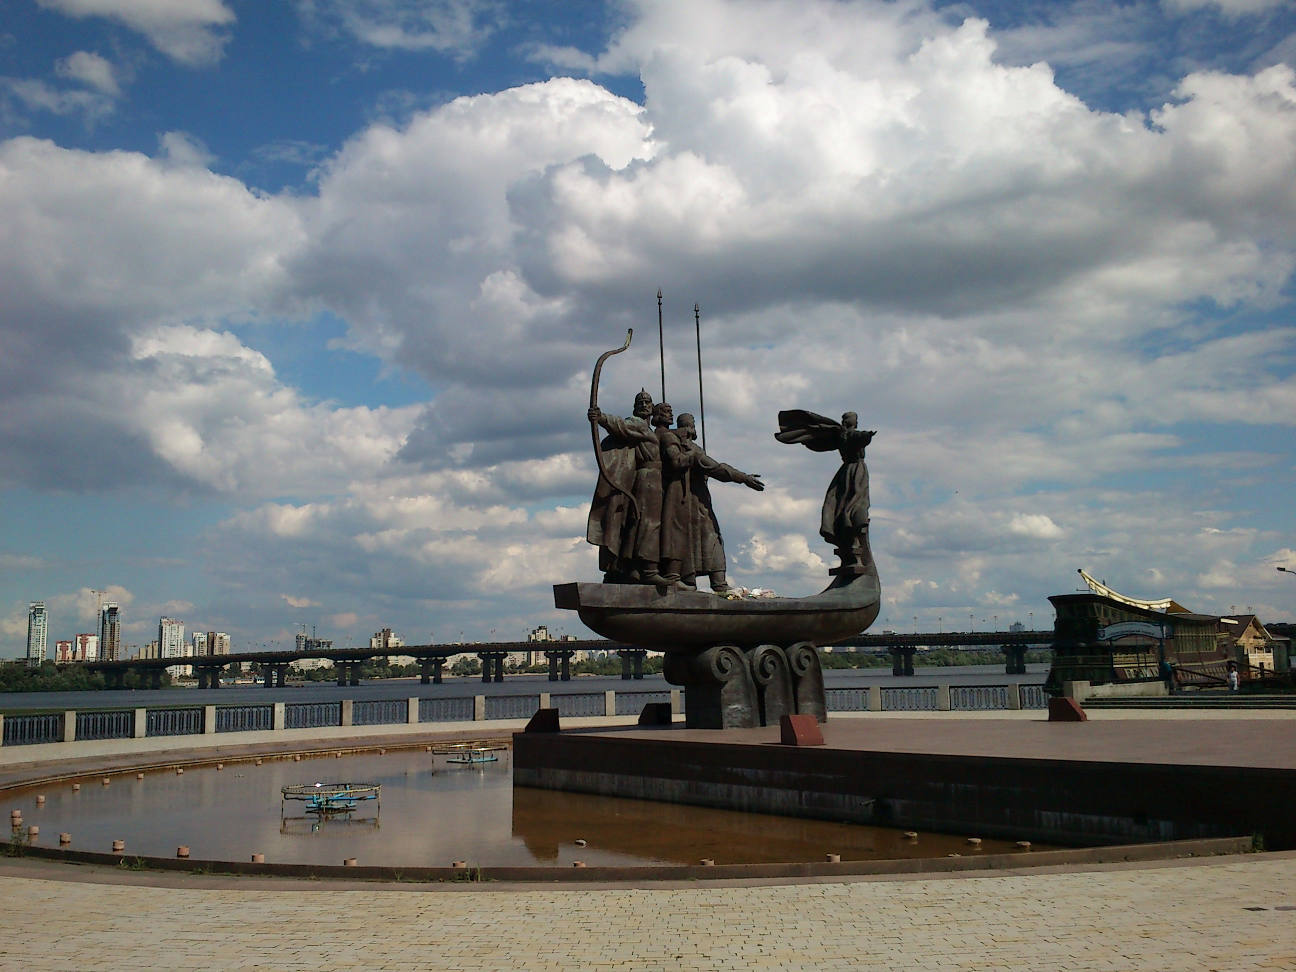
\includegraphics[width=\linewidth]{chast-colebanie-osnov/nachalo/ladiya.jpg}
\end{center}

%Небольшая модель этого памятника в промежутках между похищениями стоит во дворе Художественной академии на улице Смирнова-Ласточкина. Она же Вознесенский спуск. Нынче трудно писать книги – улицы переименовывают туда-сюда, не уследишь. Здесь и далее придерживаюсь старых, привычных мне названий., %ибо не могу переписывать книгу согласно каждому новому решению городского совета!% За исключением, когда новое название нравится мне больше.


%Там же в усадьбе академии, многие хозяйственные постройки разукрашены замечательными граффити – надо лишь завернуть за само здание с правой его стороны, к склону холма, и пройти вдоль корпуса. Пишу по памяти, может уже закрасили.

Я смутно помню время, когда лодьи со скульптурами и каменной набережной не существовало. До конца восьмидесятых, в парке Примакова был песчаный пляж, у пляжа пристань-понтон, и плавал катер на противоположный берег – южную часть острова Гидропарка, тоже с пляжем.

А под горой напротив парка Примакова разворачивался у моста Патона трамвай, что ходил вдоль древних, изрытых пещерами и сочащихся рыжими родниками холмов с Лаврой и Аскольдовой могилой, по набережной до Красной, ныне Контр\'актовой, площади. Этот чудесный маршрут упразднили. Печатно обещали – временно, оказалось – навсегда. Рельсы продержались, ржавея, дольше трамвая. На моей памяти он был одновагонный, красный.

\begin{center}
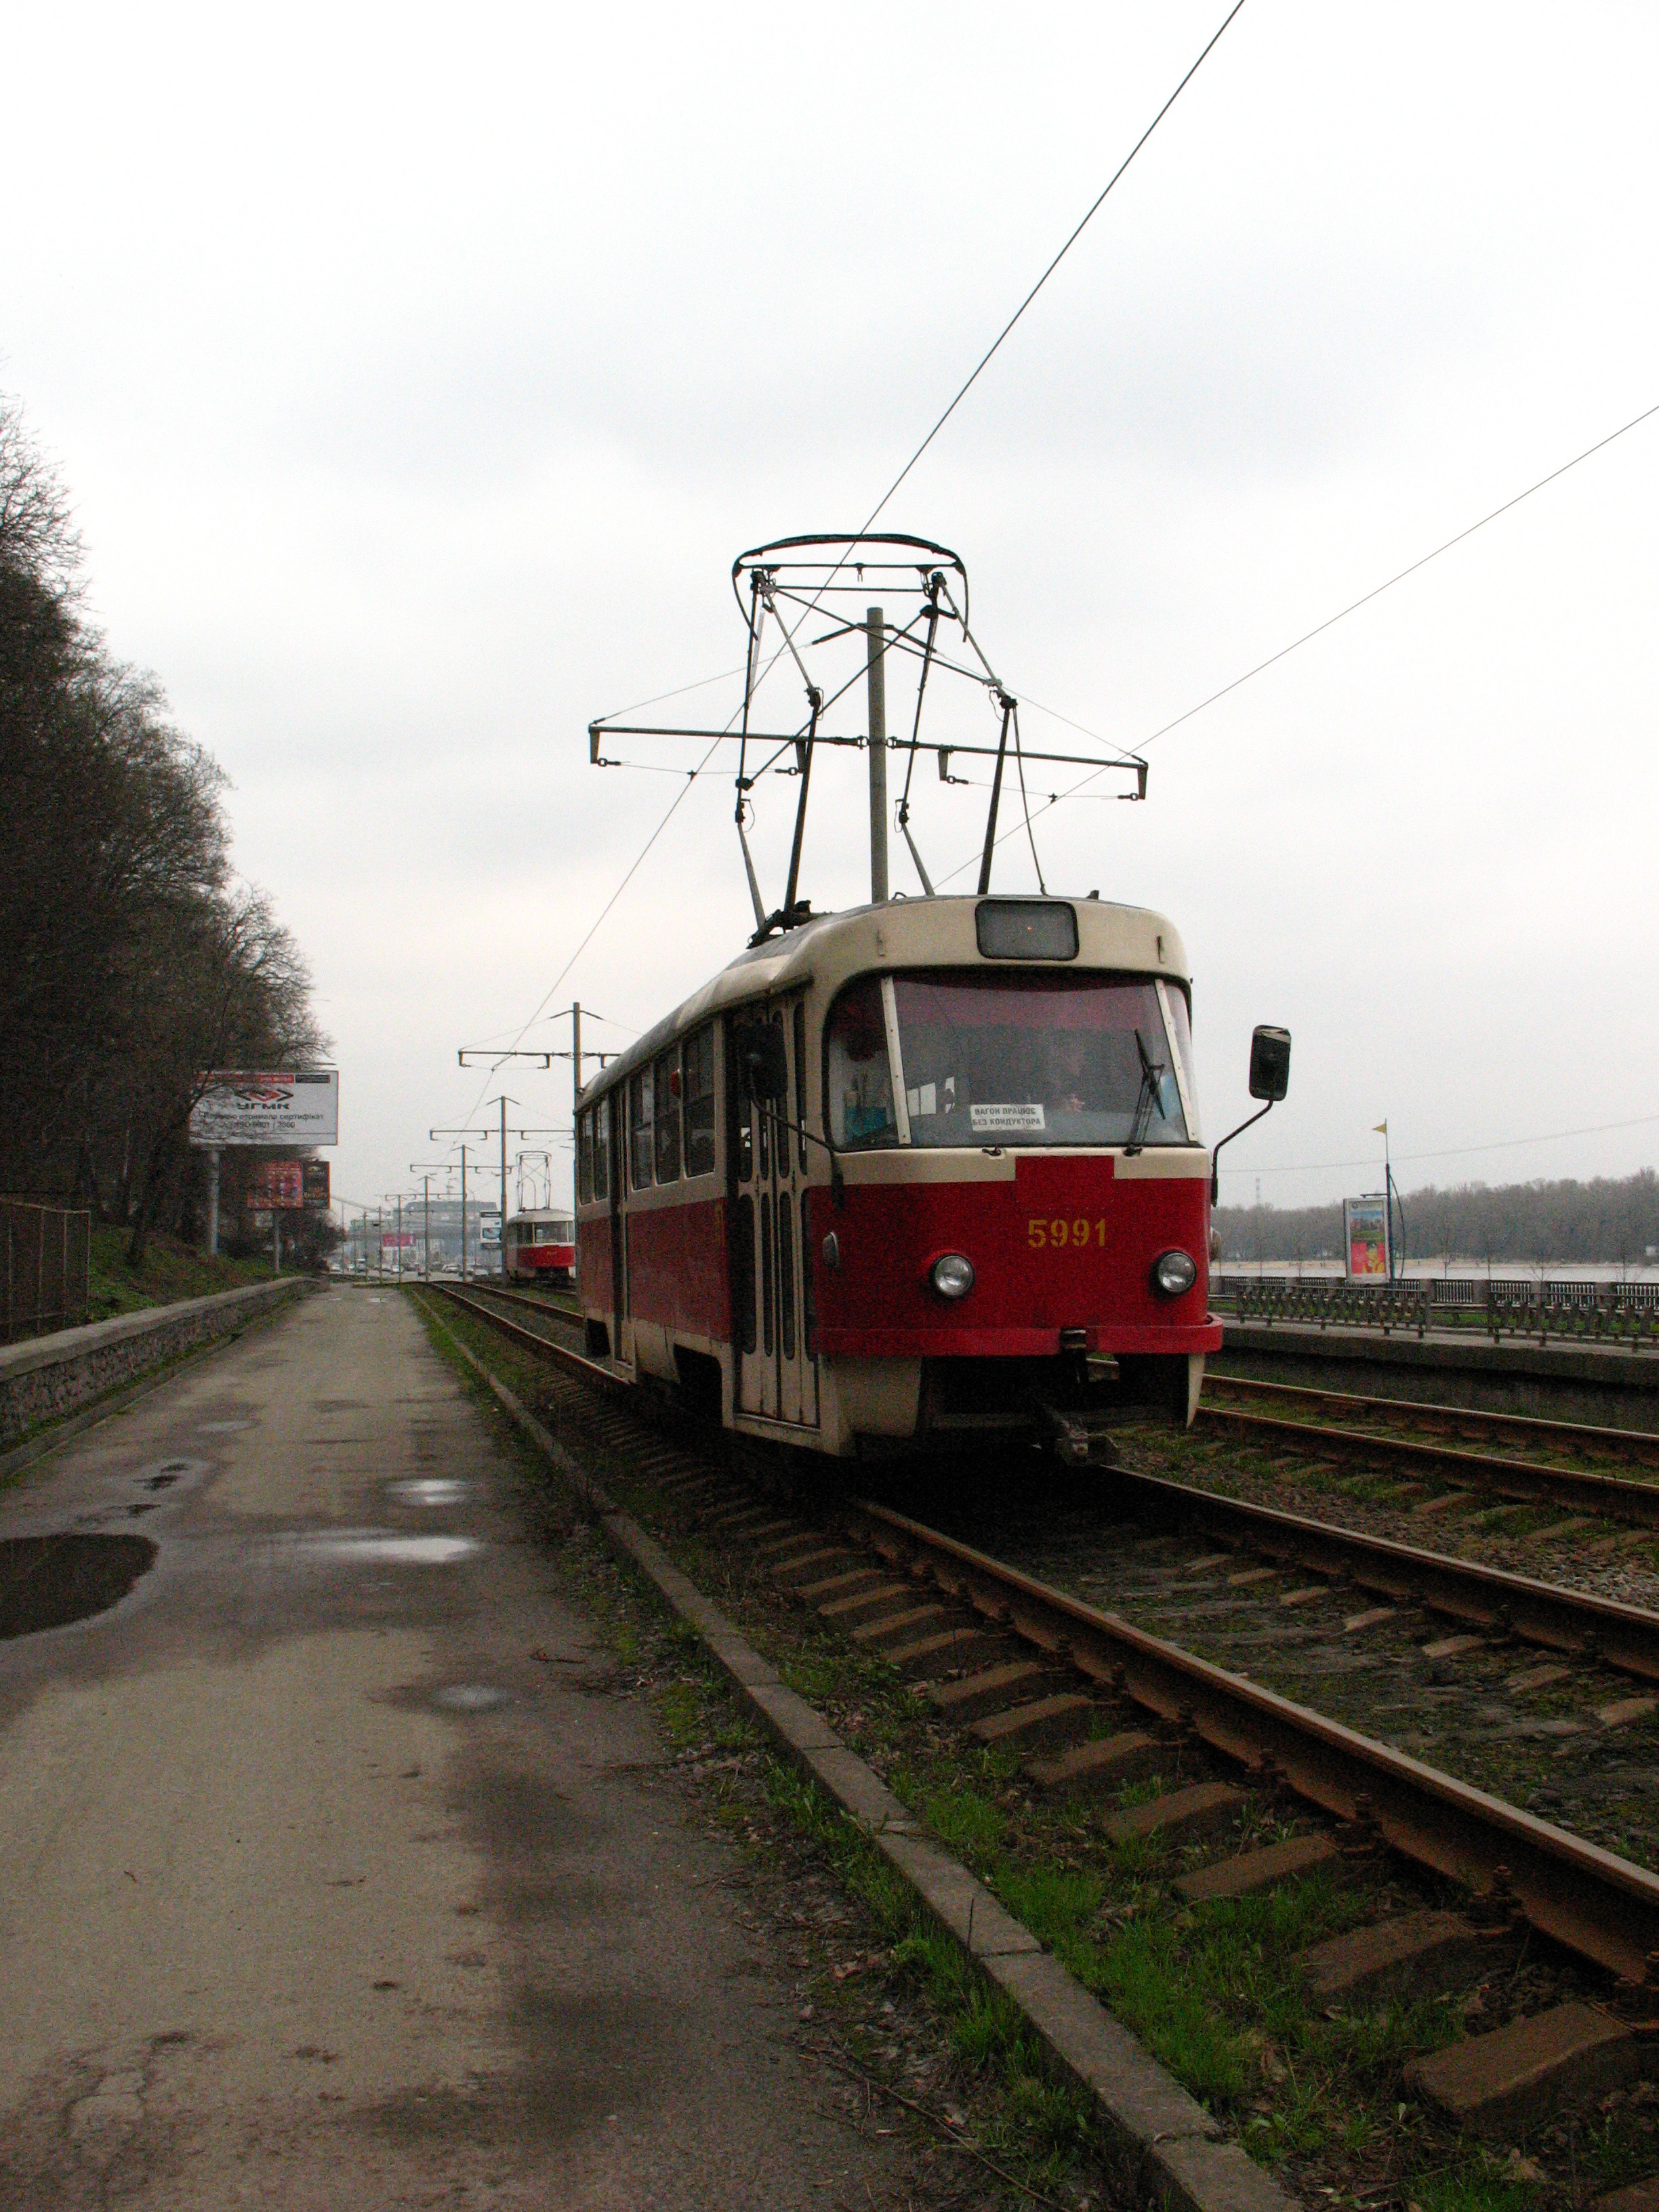
\includegraphics[width=0.70\linewidth]{chast-colebanie-osnov/nachalo/tramvay-no-5.jpg}

\textit{2008 год, на пятом маршруте трамвай «Татра» модели T3 или T4SU.} 
\end{center}

Кто не в курсе – трамвай ходил и по мосту Патона. Маршрут номер 27\index{Трамвай №27} длился от бульвара Перова до Дворца спорта, это 17,4 километра, что проезжалось чуть больше чем за час. А 35-й\index{Трамвай №35} маршрут начинался на Березняках, был разворот там где сейчас высотки возле Русановского канала, ближе к железной дороге – и заканчивался у Центрального вокзала на правом берегу. Под горой со статуей Родины-матери, около моста Патона, был большой пересадочный узел. Одна ветка шла по набережной Днепра, другая по мосту, и дальше тянулась мимо холма с музеем ВОВ и по улице Старонаводницкой, Клову и дальше в центр.

Сидишь себе да глядишь в окошко, а колеса гремят по рельсам. Печка греется. В тех старых трамваях хорошо думалось. Нынче не то, и огурцы уже не те, и пупырышки на них фуфло против давнишних.

%Но что делает капитализм с удобными и длинными маршрутами трамвая? Он их отменяет и разбивает путь на мелкие отрезки, чтобы вы делали больше пересадок. Готовь деньги! Кроме того, упраздняется сам трамвай и людям предлагается ездить в маршрутных такси. В свою очередь длинные маршруты и этих передвижных иконостасов отменяют в пользу коротких – теперь уже коммунального транспорта. Та же хитрость на новый лад.


\begin{center}
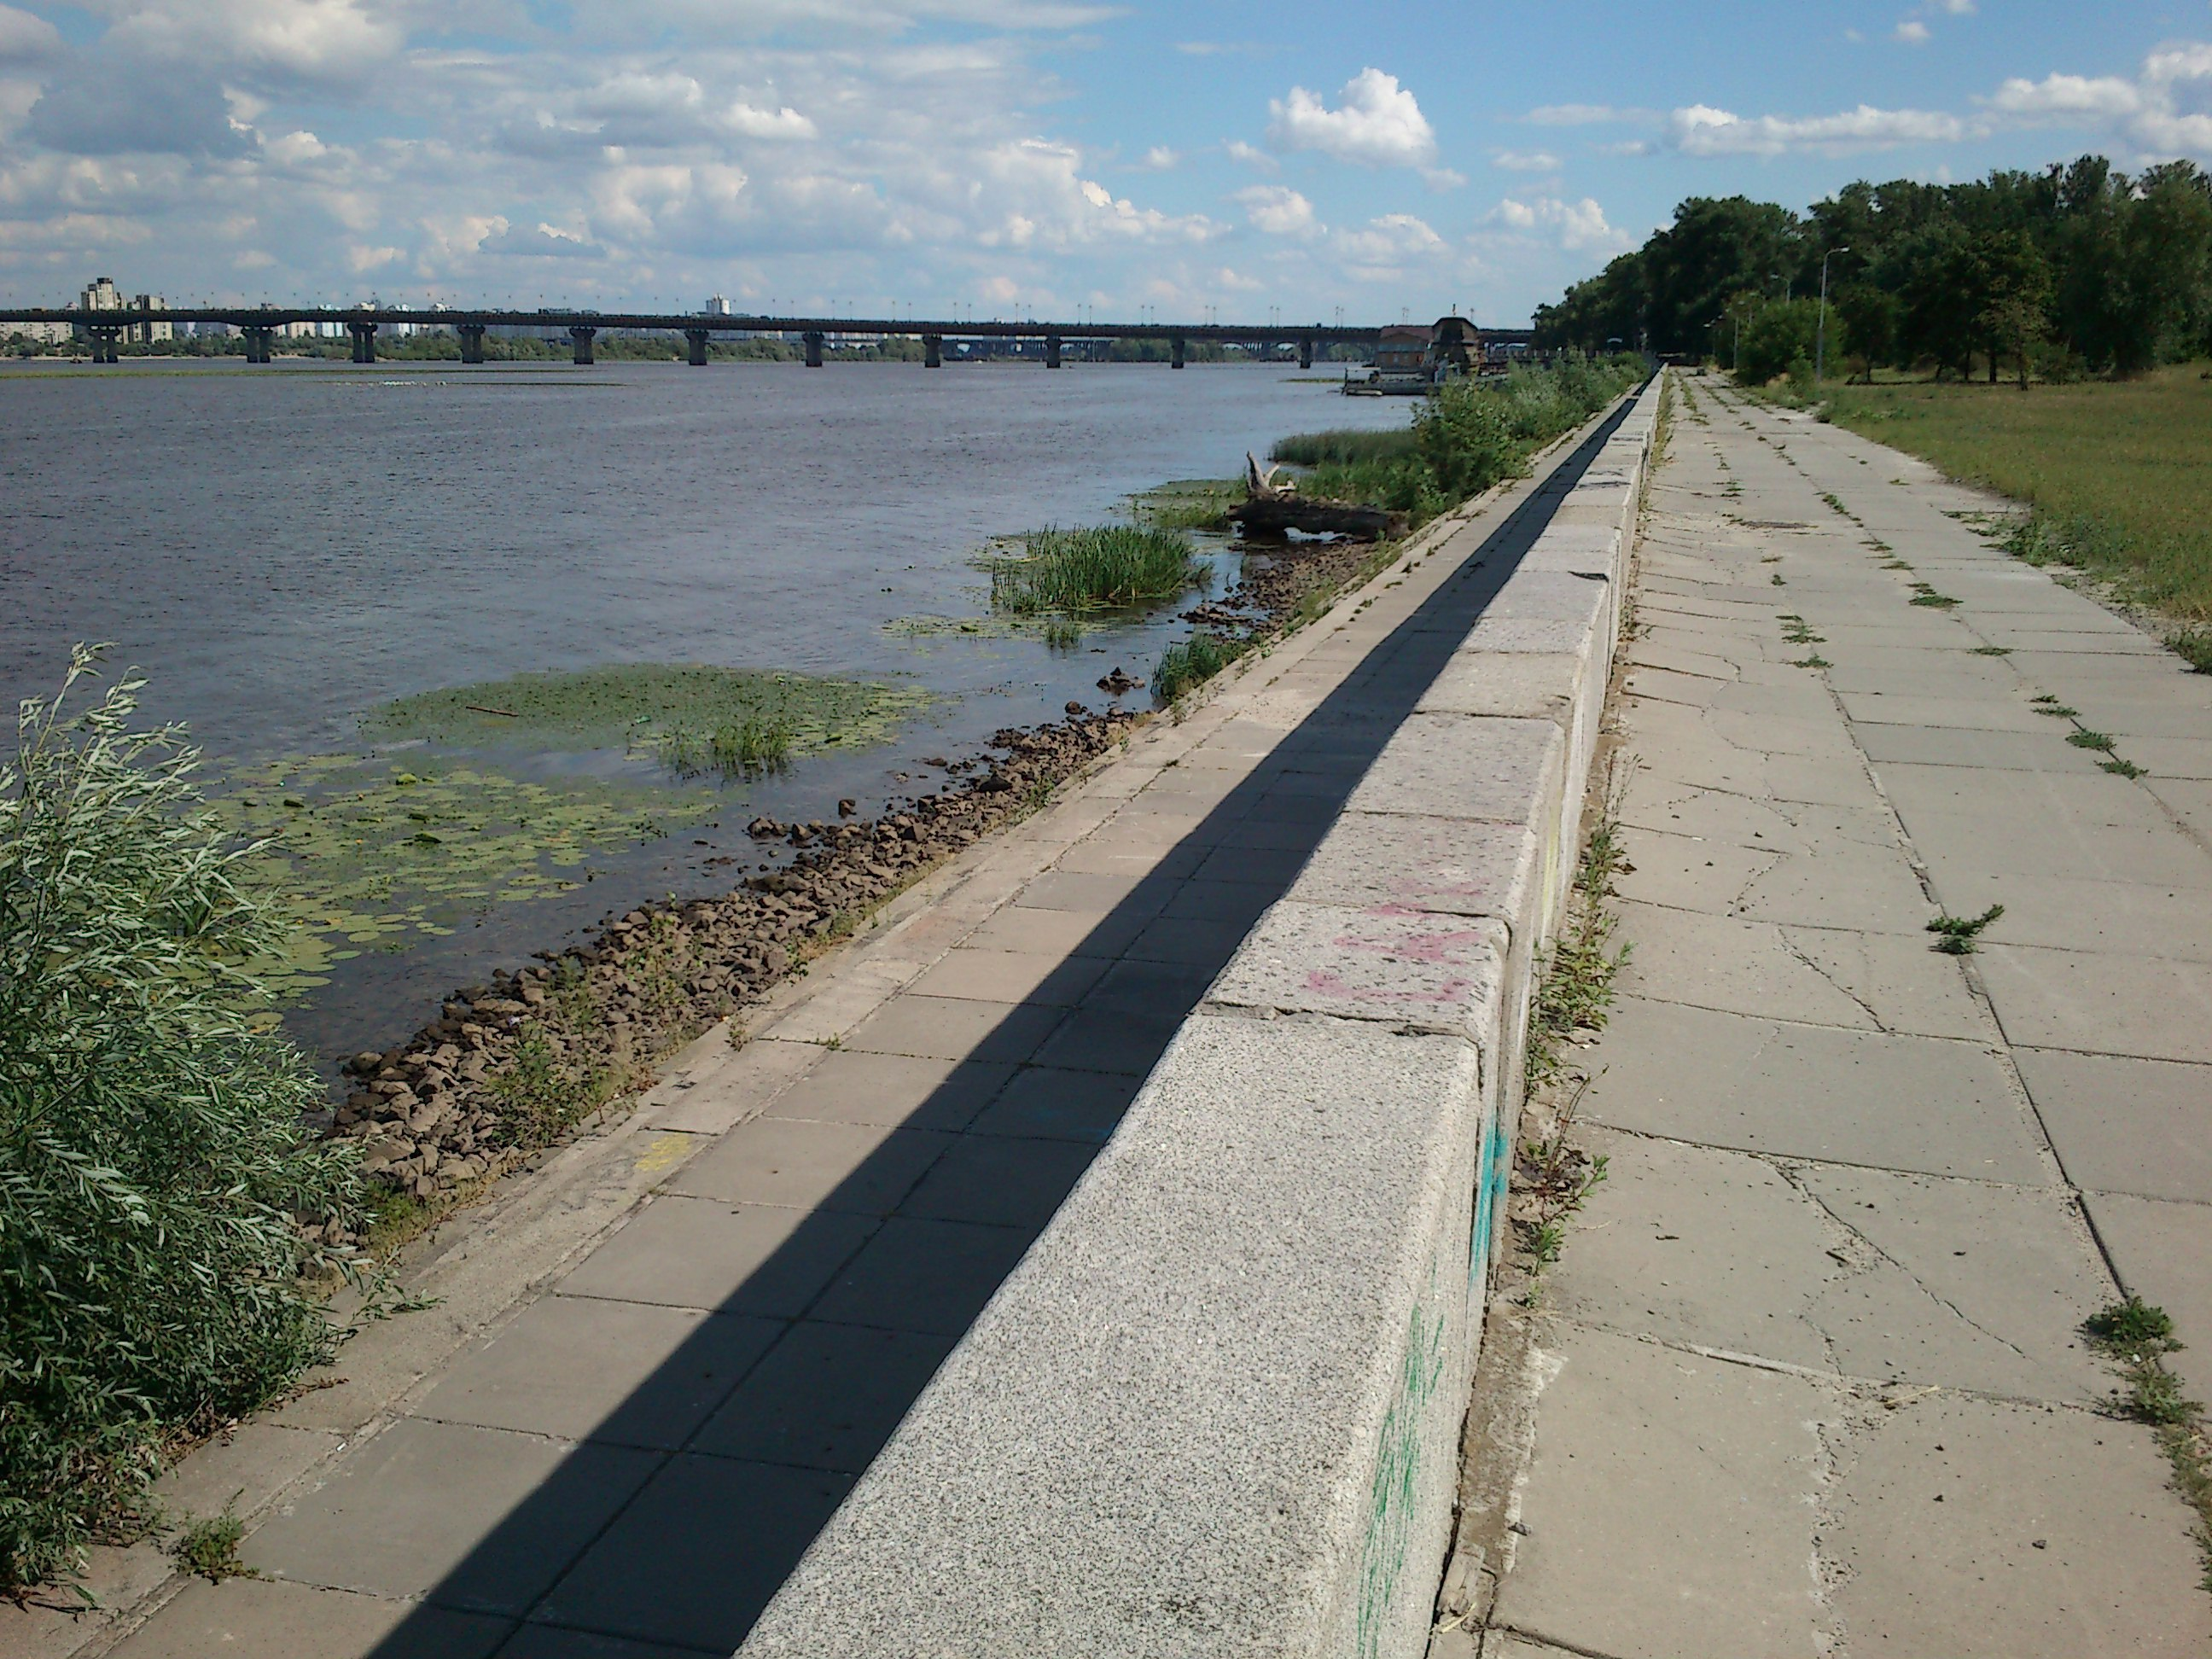
\includegraphics[width=\linewidth]{chast-colebanie-osnov/nachalo/primakova-01.jpg}

\textit{Парк Примакова, лето 2012 года.} 
\end{center}

В первом десятилетии нашего века, парк Примакова переименовали в Наводницкий и отчекрыжили от него кусок под аллею Славы миротворцев ООН. Некогда тихий парк вдоль реки, с высокими тополями и яркими цветочными клумбами, ныне застроен культовыми сооружениями, а у берегов стоят плавучие рестораны. И едут, едут машины по аллеям.

В девяностых я часто гулял там с Бобиком, моей собакой. Мы спускались туда с холмов Зверинца, от Бастионной улицы\index{Бастионная улица}.

Вот так выходишь утром из дому, а во дворе ни души, а тишина, и тепло – потому что весна и май начался. Проходишь через Собачку\index{Собачка} – крутой, продавленный глубокими ярами склон горы, весь поросший одичалыми садами. Вишня в белом цвету. Налево от Собачки, к Бастионному переулку – обрыв с бетонной подпорной стеной, за нею топорщится из ямы белопанельный Дом художников.

Там обитали художники, а их мастерские глядели широкими окнами в самое небо на высотах последних этажей. Кроме прочих жил в доме том странный человек. Он бросал с балкона вещественные плоды раздумий в пакетах из плотной бумаги, перевязанных шпагатом, эдакие бандерольки случайным прохожим.

Так уродство соседствовало с прекрасным – с сосредоточенными творцами, цветущими деревьями, и той сладковатой душистой смолой, которая сочится из узловищ в стволах вишен. Всё время забываю, как эта смола называется, а это вдруг вспомнил – камедь.

На Собачке есть две главные тропинки. Верхняя вдоль забора ботсада (мы его называли «ботаника» или «боташа»), а нижняя примыкает к опорной стене. Еще две сохранившиеся служат для подъема, в начале и конце Собачки. По ним, особенно той, что близ родного двора, я любил кататься на санках.

Нижняя тропа сейчас совсем запущена – ее перегораживает бурелом, а когда-то там свободно гоняли на велике. Посередке тропы был пятачок, широкое место, и оттуда лесенка наверх, к спортплощадке. Лесенка из деревянных, вбитых в землю дощечек. Ее делал художник Михаил Фомич, фамилию не помню. Он жил прямо напротив этого пятачка. На 2024 год и след той лестнички простыл...

Словом, по нижней тропке, кажется, никто больше не ходит, это трудно. Полагаю запустение оттого, что улица Мичурина, к которой, по сути, добирались по нижней тропе жители верховий Бастионной улицы, претерпела смену населения – давний частный сектор застроили теремами новые здесь люди.

А вот верхняя тропа осталась, утоптанная, по ней и к ней ходят в поисках дырок в ботсадовском заборе.

\begin{center}
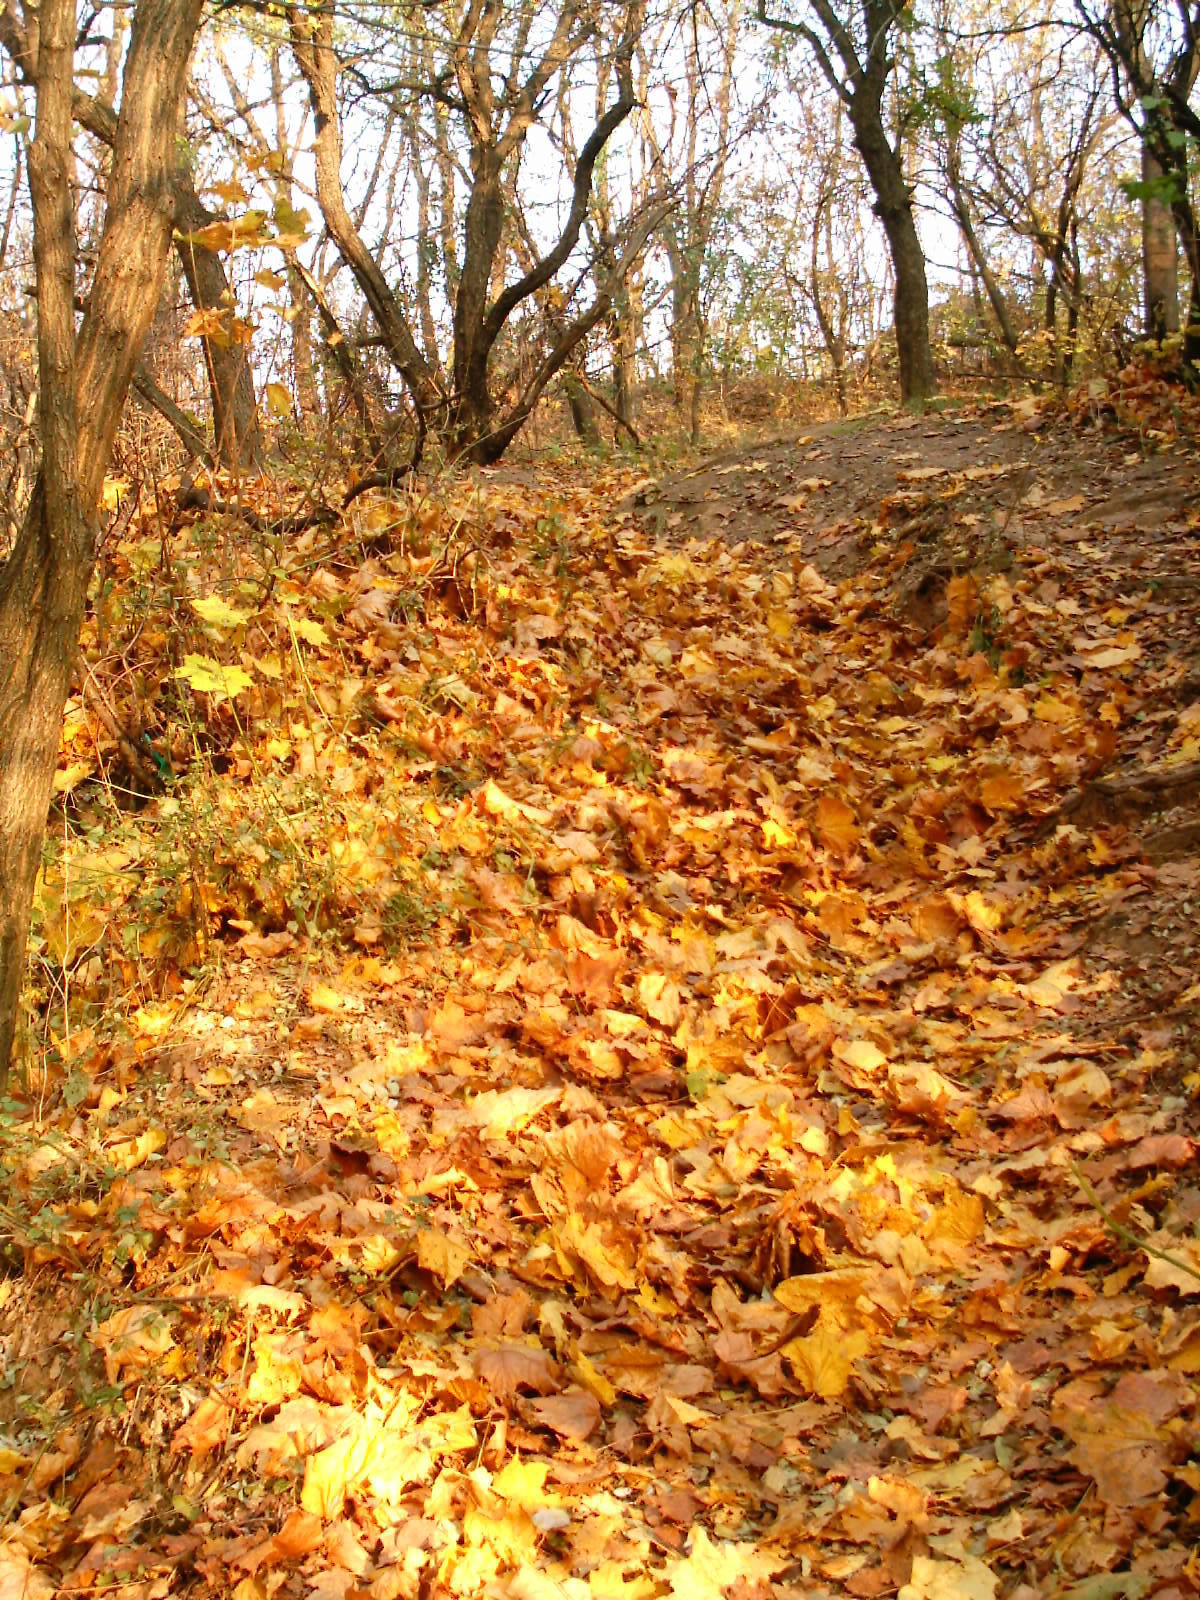
\includegraphics[width=0.85\linewidth]{chast-colebanie-osnov/nachalo/sob-imag0038.jpg}

\textit{Собачка, путь наверх, 26/10/2005.} 
\end{center}

А тогда! Зимой, вечером уже, когда тишина стоит и небо светлое от снежных туч, а фиолетовый снег искрится золотом, летят санки вниз накатанным по тропе желобом, повторяя все изгибы обрыва, и не надо рулить и тормозить, только в конце ежели не успеваешь повернуть левее, продолжая ход в желобе, то выбрасывает тебя в приземистые вишни, почти кусты, и санки в них застревают, а ты проваливаешься через ветки дальше. На верхней, посадочной площадке, у забора ботсада, растут орехи. Потом проезжаешь под грушами. И наконец – вишни!

А вот летом идешь по нижней тропинке, а из кустов высовывается сумасшедший с отверткой-заточкой. И потом исчезает, собаку увидав. А то еще находишь там же здоровенный разводной ключ, который по сей день исправно служит.

На Собачке было ровное место со спортивной площадкой с оградой из сетки. Туда, по террасам среди диких вишень, поднималась лестничка Михаила Фомича, переходившая в грунтовую дорожку. На площадке стояли даже тяжелые металлические футбольные ворота, а на возвышении в рост человека, таилась под сиренью скамейка. Местные играли тут в футбол, выгуливали собак, а на лавке заседали любители поиграть на гитаре.

Еще в конце девяностых, со спортплощадки украли ворота. Сначала одни, потом вторые. Затем, по мере удаления от социализма, исчезали покрывшиеся ржавчиной части ограды, глинистая полянка зарастала травой, ползла вниз зелень с пригорка, уже не сирень, а нечто совсем дикое.

Северная сторона Собачки выходит ко глубокому яру. На противоположном его берегу – остатки погребов. В начале 21 века в них жили беспризорные дети. Затем погреба пришли в совсем удручающее состояние, а яр усеялся мусором. Выше погребов начинается частный сектор на улице Мичурина.

От Собачки мы с Бобиком, пройдя мимо нескольких «гостинок» и сойдя по лестничке у некогда единственной в районе шестнадцатиэтажки, сворачивали на эту улицу. Она тогда была очень мирная, с гнилыми, косой гармошкой, деревянными заборами, за них лезла лапами наружу сирень. В гуще садов прятались домики. Летом на ходу вишню в рот отправил, водную колонку близ обочины покачал, горстью выпил студеной воды – и дальше. Редкий прохожий встретится.

Нынче там – современные терема и бетон, и должен вжиматься пеший человек в новокрепостную стену, чтобы не быть смазанным в месиво не то машиной, не то танком, принявшим облик автомобильный. Раньше название улицы вполне оправдывалось её зеленью – и наверное, были в садах сорта, выведенные самим Мичуриным. А рядом с теремами садов нет. Поставят эти кусты-пудели и наймут садовника, чтоб их подстригал. Барскому глазу приятно смотреть.

\begin{center}
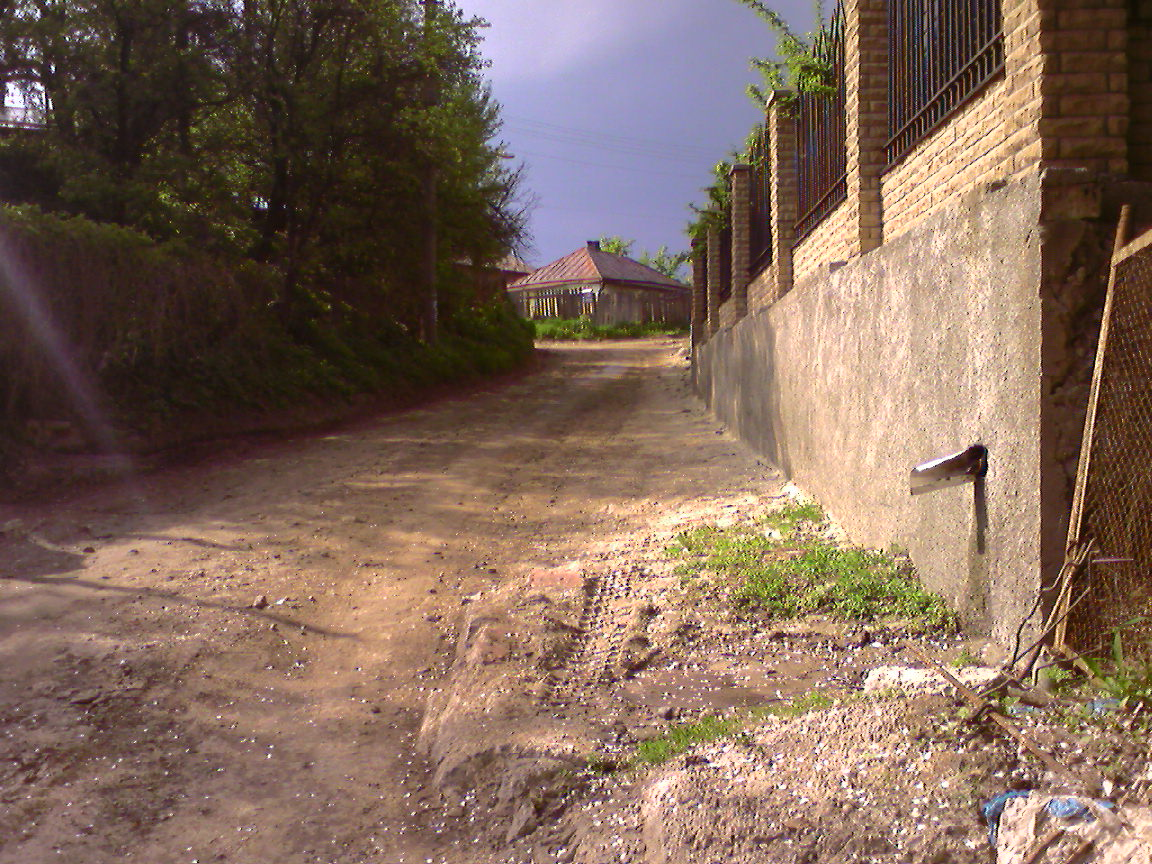
\includegraphics[width=\linewidth]{chast-colebanie-osnov/nachalo/lomakovskaya01.jpg}

\textit{2006 год, улица Мичурина, впереди – перекресток с Пирятинским переулком.} 
\end{center}

Улица Мичурина, бывшая Ломаковская, по крайней мере с 18 века
идет в устроявшихся пределах по всему склону северного Зверинецкого холма, посередке его ската, вбирая в себя узкие улочки и переулки, лестницы и лестнички. Одинокая скамейка ближе к перекрестку с Пирятинской улицей наводила на мысль о каком-то редком автобусике, что мог здесь курсировать в давние времена, как 76-й маршрут\index{Автобус №76} по Зверинецкой, хотя крутизну гор на Мичурина, кажется, не сможет преодолеть ни один автобус.

На моей памяти, не было там и магазина, а лишь частные усадьбы, водяные колонки, просмоленные деревянные столбы, синие почтовые ящики на множество дверок, да две таксофонные будки. Одна, почти в начале Мичурина, около лестнички под шестнадцатиэтажкой, прославилась тем, что в ней укрылась от разозлившегося козла какая-то бабка. Козел всё же проник внутрь и бабка сдерживала его, ухватив за рога. Другая будка стояла подле перекрестка с Пирятинской. 

\begin{center}
\includegraphics[width=\linewidth]{chast-colebanie-osnov/nachalo/\myimgprefix 13092009653.jpg}

\textit{2009 год, улица Пирятинская, впереди – перекресток с Мичурина.} 
\end{center}

Оттуда можно было свернуть на север, в сторону бульвара Дружбы Народов. Спускаешься в тени деревьев по громадной лестнице – теперь так нельзя, улица Пирятинская прерывается посольством, и лестница прикреплена уже к нему. Внизу же, правее, в сырой ложбине холма журчал вкусный родник\footnote{50°25'25.7"N 30°33'46.9"E}, слывший целебным. Возможно, в давние времена он назывался Рожницей. Сюда в восьмидесятых-девяностых издалека приезжали с бидонами люди. И там построили автозаправку. Существа из карбона и металла хотят пить горючее. Иди дальше, зверь из плоти. Купи себе воду в баночке.

Лестницей я возвращался, домой, а в парк Примакова двигался дальше по улице Мичурина, до самого ее конца, где очень крутой спуск. Однажды я съехал с него, полностью заледеневшего, на санках. Здесь застройка новоделами началась раньше всего.

\begin{center}
\includegraphics[width=0.80\linewidth]{chast-colebanie-osnov/nachalo/\myimgprefix IMG_20150601_133144.jpg}

\textit{2015. Спуск на Мичурина. Прежде, слева были сады за деревянными заборами, а справа – поле с подсолнухами.} 
\end{center}

И вечно до половины этого спуска доходили, темня треснутый асфальт и камни, ручьи – то ли родники, выбивающиеся из-под люков, то ли вода, накачанная из колонок.

Вообще этот отрезок улицы Мичурина держится за нею больше на бумаге, ибо там по прямой как бы продолжается улица Землянская. Она же прежде, взобравшись на гору, лежала и по другую сторону забора ботсада, через нынешний участок хвойных растений, отмежевывая его от сирингария. Там поныне есть аллея, но мало кто знает, что это бывшая улица.

Землянская улица вливалась в Выдубицкую, что еще начале сороковых годов двадцатого века пересекала всю местность будущего ботсада примерно от Бастионной улицы и до Выдубицкого монастыря. И перекресток Землянской и Выдубицкой был там, где сейчас перекресток у верха Сиреневой аллеи, с поворотом к хвойным, сирени, Ионовской церкви да назад к выходу из ботсада.

Старые домики на Мичурина держалась долго. Я ходил по улице из года в год – ничего не менялось.

Но вот одна из усадеб обезлюдела. Пустые висели меж яблонь качели. Стала врастать в землю калитка, за несколько лет одичал сад, хотя соседи еще пользовались его плодами. Сам домик вначале сохранял жилой вид, а потом просела над входом крыша, треснули, принялись осыпаться стены – через отвалившуюся штукатуру проглядывала дранка, косая решетка из досочек. 

Этот единственный на улице выбывший из строя дом оказался предвестником грядущей волны таких угасаний с последующим пришествием новых хозяев. А те выкорчевывали сады, срывали части склона для умещения огромных фундаментов строящихся жилищ.

Не люблю больше бывать на Мичурина. Пусть остается в моей памяти какой была. До соединения с Землянской, улица поворачивала и круто спускалась, там еще на пригорке справа стоял деревянный дом – номер сорок? Всё это срыто, даже сама улица теперь смещена.

Землянская и одноименный переулок напоминают о местности Землянке, прозванной так по близости к Зверинецким пещерам, либо от земляных укреплений Зверинецкой же крепости, что некогда покрывала многоугольником валов половину нынешнего ботсада и сгинула окончательно при его строительстве в 1940-х.

Пещеры на моей памяти сначала были закрыты для посещений. Не стояли рядом две церкви, всё выглядело иначе. Вход располагался в обычной частной усадьбе на Мичурина. В шестидесятые к нему приладили будку туалета, которую потом передвинули по просьбе археологов. А в конце девяностых в пещеры начали водить паломников, сверху горы, через проем в стальном, из ребристых прутьев, заборе ботсада.

Там рядом с плантацией кормовых культур был плоский участок, куда свозили торф – как понимаю, место дореволюционной церкви над пещерами – и вот за торфом пропилили в ограде большую дырку, может даже с калиткой, не помню. Потом уже подключился близлежащий Ионинский Святотроицкий монастырь и в нулевых на месте нескольких частных усадеб возвели Архангело-Михайловский Зверинецкий монастырь. Сами же пещеры утратили свой исконный вид еще в начале 20 века, будучи приспособленными для паломников. Сейчас это еще более облагороженное подземелье.

Назову основополагающие работы про эти пещеры, тоже начала 20 века.

Полная чудес брошюра иеромонаха Серапиона «Новооткрывающиеся древние пещеры в Киеве, на Зверинце», вышедшая в Киеве в 1914 году. 

Банковский служащий и одновременно опытный археолог Александр Дмитриевич Эртель\footnote{Много изучал киевские курганы, пещеры, валы и городища, в том числе пещеры в Китаево, курганы в Совках, могильник около Проневщины. К слову, брат Эртеля, Леонид, с 1914 года проживал на Ломаковской (или по Ломаковскому переулку), 37-А.}, крайне правый монархист, написал в 1913 году брошюру «Древние пещеры на Зверинце в Киеве».

Киевский историк Иван Каманин\footnote{Каманин оглох после болезни, что повлияло на выбор рода деятельности – работу в Киевском центральном архиве древних актов. Много печатался в дореволюционных околоисторических изданиях под своей фамилией и псевдонимом А. Щуровский. Каманина, согласно завещанию, в 1921 году похоронили в тех же Зверинецких пещерах – одна из стен его склепа, кирпичная, граничит с концом «Алтарной улицы».} год спустя выпустил более объемный труд «Зверинецкие пещеры в Киеве»\cite{kamanin01}.

И в 1918 году профессор Киевской Духовной Академии Николай Петров подытожил работы Эртеля и Каманина, добавив кое-какие источники, книжечкой «Ученые труды по исследованию ново-открытых в Киеве Зверинецких пещер».

%Везде, где рассуждений больше, чем описания, возможно искажение сути, возникающее в мыслях сочинителя. Логические ошибки, невнимательность, наконец личное мнение, окрашивающее любые рассуждения и зачастую отсекающее ряд доводов – всё это вносит путаницу, а путаница, в отличие от кругов по воде от камешка, не угасает, но увеличивается – чем дальше от источника, тем она сильнее. Но хуже всего, когда пытаются исправить первоисточники, полагая в них ошибку – это приводит к ошибке еще большей.
 
Многократное открытие древних Зверинецких пещер в конце 19 и начале 20 веков – дело весьма запутанное, обросшее искажениями и домыслами, возможно порой намеренными, а иногда случайными, по недостатку сведений – ведь кроме упомянутых мною источников, притом довольно редких, данные о пещерах, по большому счету, отрывочны и порой не заслуживают доверия.

%Кратко сведу воедино самое важное. Не буду принимать по внимание голословные сведения из статей, вроде того, что в пещерах были найдены какие-то кожаные и деревянные маски – я не знаю, откуда это взяли. Можно еще услышать версию, что в пещерах обитали монахи Выдубицкого монастыря еще до его наземного устроения. На это нет никаких указаний. 

Кратко сведу воедино самое важное, чтобы дать представление о том, какими были Зверинецкие пещеры на стыке 19-20 веков, а не какими их теперь показывают.

Летописи и другие давние письменные источники про эти пещеры загадочно молчат. Вообще. Тут несколько вариантов. Например, пещеры относилсь к дохристианским временам и при летописцах и сочинителях житий были уже засыпаны, неизвестны, не обжиты позднейшими монахами. Или – летописцы знали о пещерах, но молчали о них, считая нехристианскими или не совсем христианскими. В том и другом случае христианская атрибутика могла попасть туда позже, с умыслом доказательства религиозной принадлежности пещер. Наконец возможно, о пещерах, пусть даже там был монастырь, не упоминали из-за их незначительности. Но последнее кажется мне натянутым, ведь летописи пестрят сообщениями о помощи того или иного князя в устроении церкви или монастыря. А про Зверинецкие пещеры – глухо.

В обозримом прошлом о них узнали, по большому счету, только в 19 веке. По словам Каманина, весной 1882 или 1883 года в склоне горы, при обвале, открылся ход. Подробности всплыли уже в начале 20 века, когда о событии тридцатилетней давности поведала восьмидесятилетняя местная жительница, повитуха Феодосия Матвеенкова\footnote{Справочник «Весь Киев» за 1911 год снабдит нас её адресом: «Ломаковская, 10. Матвеенко Федосья Вас.». В 1913 году обвалилась земля и в усадьбе Юлиании Хмелько по адресу Ломаковская, 12 – там был проход в подземелье, раскапываемое археологом Эртелем.}. Каманин пересказывает старожилку, пользуясь книжечкой 1914 года иеромонаха Серапиона «Новооткрывающиеся древния пещеры в Киеве, на Зверинце»:

\begin{quotation}
на рассвете одного дня, ровно 32 года назад\footnote{Т.е. в 1879-м.}, слышала гул провала земли и видела светлую радугу, которая упала на месте провала. В полдень того же дня сосед Матвеенковой, живописец Дмитрий Зайченко\footnote{Усадьба на имя «Зайченко Мар. Владимир» на 1911 год обозначена по адресу Ломаковская, 9.}, с своим товарищем, возвращаясь из Свято-Троицкого монастыря, заметил провал. Они разрыли отверстие провала, и Зайченко спустился в образовавшуюся яму, где пробыл около 15 минут; при свете восковой свечи он обнаружил длинную пещеру, в которой, по его словам, было много человеческих голов, костей, неистлевших остатков монашеских поясов, четок, обуви и т.п.
\end{quotation}

У Серапиона про радугу более подробно:

\begin{quotation}
Явление радуги во сне

В 1878 или 9-м году весною, будучи восприемницею младенца в доме №6 по Ломаковской улице у Ксении Лобановой, Феодосия, после приема мальчика, на рассвете легла отдохнуть в комнате на кушетке против северного окна. В легкой дремоте ей представилось, что с северо-запада идет очень низко над домами большая и широкая радуга и страшно гудит: гугу, гугу!... И прошла по направлению к ея дому и, спустившись, пала за забором ея усадьбы на склоне горы, где впервые потом обнаружились пещеры.

С этого ужаса она пробудилась и стала собираться домой, чтобы удостовериться, не случилось ли пожара, или другого несчастья в ее доме, или усадьбе. Но Лобанова уговорила ее остаться у ней до полного рассвета и не тревожиться зря сновидениями. Когда же развиднелось, она пошла и осмотрела дом и усадьбу и нашла всё благополучным.
\end{quotation}

Некоторое время спустя после обнаружения пещер, Матвеенкова видела еще такой сон – в ее усадьбе, около входа в пещеру, под большим орехом стояло человек пятнадцать монахов, в белой одежде, с непокрытыми головами и распущенными, стало быть длинными, волосами. Это противоречит внешности монахов вообще – те одеваются в черное и носят головные уборы. Но, пусть будут монахи. Они стояли, стонали и просили: «Покормите нас».

Матвеенкова хотела заказать в своем саду панихиду, говорила об этом с приходским священником Иоанном Вышатой и знакомой своей, Сиклитией Николаевской. Что-то такое было в разговорах и вообще людской молве вокруг, и Матвеенкова отступилась от мыслей от панихиде. Создается впечатление, что тогда, в то время, обнаруженные останки, да и пещеры тоже, не считались христианскими.

Спустя много лет, в 1902, Матвеенкову снова посетило видение – опять же, на грани сна и яви она увидела женщину с дитятей на правой руке, склонившим голову ей на плечо, и подумала, что это женщина из пещер. Серапион пишет: «видела покойницу ясно в лицо – волосы у нее не то седые, не то цвелые и прилипшие к телу, и вид ее тощий, худой и мертвый, будто бы только что из гроба вставши». Гостья напомнила, что Матвеенкова обещала покормить их, но не исполнила обещанное. Матвеенкова пошла в чулан за молоком, оглянулась, но «покойница» исчезла. А Матвеенкова таки заказала в Троицком монастыре панихиду.

Далее в книге мы еще коснемся странных видений на грани сна, бывающих у повитух всех народов, пока же вернемся к событиям на Зверинце. Да – конечно сказанное далее уместнее будет разместить в главе, где речь пойдет о Святотроицком монастыре более подробно, но поскольку речь зашла об аномальщине, то... К тому же Зверинецкие пещеры по многим прикидкам тянулись и к этому монастырю.

Расположен он от пещер всего в шестиста с гаком метрах на юго-восток, в ботсаду. Ионинский Святотроиций монастырь, известный также как Ионинская церковь. Иона, основатель оного в 19 веке, поведал в воспоминаниях своих о месте, где позже возник монастырь:

\begin{quotation}
Строения здесь никакого не было, одна земля и заросли. Отец Иларион сделал себе куренёк из хвороста, нарванного здесь же, из дикого бурьяна сделал крышу и жил  в нем целое лето, а потом Бог благословил, и появилась маленькая келлейка на чистом, не заросшем месте. 

Купив барочного леса, я поставил из толстых бревен столбы в углах, а стены из досок длиною и шириною 7 аршин, она и теперь стоит\footnote{Была позже разобрана.}. 

В этой келлии мы жили двое. Я вышел из Греческого монастыря и до поступления в Выдубецкий жил в этой келлии с о. Иларионом.

Здесь был сад, в котором росли разные фруктовые деревья: груши, яблоки, сливы, вишни, орехи. Место это было отгорожено от Выдубецкого монастыря забором и по уличке внизу шириною 7 сажень.

Когда о. Иларион здесь жил один, он видел выходящее из земли пламя, охватившее всю местность, где ныне стоит малая церковь. Видел огненный столп огромный, доходящий до небес, столп виден был даже на горе, где ныне собор.

Много ему было страхов от диавола. Диавол гнал его отсюда. К нему приходили неоднократно  воры и грозили убить его, но Бог его во всем хранил и укреплял. Диавол поносил его и говорил, зачем он здесь живет, лучше жить в монастыре, чем здесь. Диавол рыдал всю осень, зиму и весну, ходя по переулку и кляня о. Илариона, Николая и Романа, которые жили втроем, приговаривал: «Проклятые черноголовые, длинноволосые калугеры зудят мне, гонят меня и покою мне не дают, из наследия моего древнего и давнего гонят меня». Все это слышали братия и терпели.
\end{quotation}

Малая церковь – это старая, почти кубическая, двухэтажная колокольня\footnote{50°24'57.9"N 30°33'47.2"E}. Она стоит почти на краю холма позади своей копии, новой колокольни. От старинной, вниз на другой уступ холма ведет бетонная лестница, упираясь в тыл полуразрушенного на 2020 год, добротного дома в три этажа.

\begin{center}
\includegraphics[width=\linewidth]{chast-colebanie-osnov/nachalo/\myimgprefix IMG_20200202_133135.jpg}
\end{center}

До революции он принадлежал монастырю, а в советское время там была школа, а затем один из научных корпусов ботсада, со столовой на первом этаже. Если встать лицом к переду дома, то справа будет виден округлый проем в холме\footnote{50.416287836193135, 30.56328794279714}. А от лестницы, как спуститься, он будет слева.

Это вход в некое монастырское подземелье вроде погреба. Обложен кирпичом, внутри просторно, от основного серединного помещения отделяются дополнительные по бокам. На 2020 год там лежит разный бесхозный хлам. А вот около самого входа любопытное. Под аркой, в левой стене зияет проем высотой чуть поболе человеческого роста. Он ведет в пещеру с низким потолком, где идти надо сильно пригнувшись.

Вырыта она в плотном суглинке. Близ входа, справа, есть ниша, где может поместиться человек. Длина пещеры метров шесть. Поначалу – а от входа высота сразу уменьшается – в ней можно стоять согнувшись. Затем высота потолка резко понижается на треть. И после понижения приходится идти на корточках. В месте понижения получается как бы обод арки, и на нем ровно отпечатан крест без диагональной перекладины. Других надписей или рисунков я не заметил. Далее по ходу еще одна такая арка, но без креста.

Стены и потолок пещеры очень гладкие, кроме самого начала, где, как видно, старый ход грубо расчищали лопатами. Поверхность стен вообще не несет на себе следов работы, ее будто отшлифовали. Потолок закруглен.

Не знаю, когда возникла эта пещера, кто ее стал раскапывать (вероятно долгое время вход был засыпан и закрыт кирпичами арки погреба), когда и как в суглинке сделали крест – создатели пещеры или ее последующие обитатели. Для жизни там человека она крайне неудобна из-за низких потолков и узости своей. Возможно, ход продолжается далее, но засыпан – в конце пещеры снова грубая обработка стен, слишком отличная от общей изящной и продуманной.

Не об этой ли пещере писал археолог Александр Эртель в статье 1920 года «Новые данные по истории Выдубицкого монастыря» следующее:

\begin{quotation}
Затем в усадьбе Троицкого монастыря вблизи церкви мы с И. Я. Стеллецким нашли весьма подозрительный ход, часть коего обращена монахами в погреб для хранения овощей.
\end{quotation}

\vspace*{\fill}
\begin{center}
\includegraphics[width=\linewidth]{chast-colebanie-osnov/nachalo/\myimgprefix IMG_20200202_132529.jpg}
\textit{Внутри пещеры, 2020 год.}
\end{center}
\vspace*{\fill}

\newpage
\vspace*{\fill}
\begin{center}
\includegraphics[width=\linewidth]{chast-colebanie-osnov/nachalo/\myimgprefix IMG_20200202_132538.jpg}
\textit{Внутри пещеры, 2020 год. Вид на ту же арку, но ближе.}
\end{center}
\vspace*{\fill}
\newpage

Так вот Илларион наблюдал аномальщину как раз на горе точно над пещерой, что рядом с описанным мною домом. Откуда наблюдал? Очевидно, не около места часовни, не с места наблюдаемого явления. А назвать то место горой можно только с двух точек – будучи около упомянутой пещерки либо с другой стороны, где сейчас сад магнолий.

Вернемся теперь в 1880-е годы и снова к Зверинецким пещерам. 

Матвеенкова была свидетельницей, как художник Зайченко исследовал пещеру – сначала он тыкал в провал палкой, потом повитуха принесла ему длинный шест, но и тот не достал до дна, наконец провал разрыли больше, и художник полез вниз с огарком свечи. Шарил там минут пятнадцать, после чего выбрался и рассказал, что видел человеческие головы, кости, да, по словам Серапиона, недоистлевшие остатки монашеских поясов, обуви, четки.

%Без ссылки на источник иногда пишут, что художник нашел также кожаные и деревянные маски. Выдумка?

Кроме Зайченко, посетили пещеры и монахи Ионинского монастыря, которые, как пишет Каманин, «кое-что оттуда вынесли» – а что именно и в каком количестве, точно неизвестно. Сам архимандрит Иона взял, по крайней мере, два черепа. Над обнаруженными в пещере останками почему-то не провели заупокойный молебен, оставили лежать как есть.

Матвеенкова со своей знакомой тоже отправились в пещеру и вспоминала потом, что

\begin{quotation}
видела там около 50 истлевших гробов в отдельных пещерках в правой стене; в каждой пещерке лежало по двое покойников головами к ея устью;

Матвеенкова насчитала 99 черепов; доходила она и до какой-то двери, постучала рукой, но отзвука почти не было, потому что снизу дверь оказалась засыпанной почти до половины землей; глядя сверху, за дверью виднелась пустота.

Дверь деревянная, покрыта толстыми листами железа, которые прибиты железными же гвоздями головками в копейку. Высота пещеры – аршина в три\footnote{2,1 метра.}, а ширина чуть уже. От двери идут еще проходы в три стороны, самая же дверь стоит на летний восток.
\end{quotation}

\begin{center}
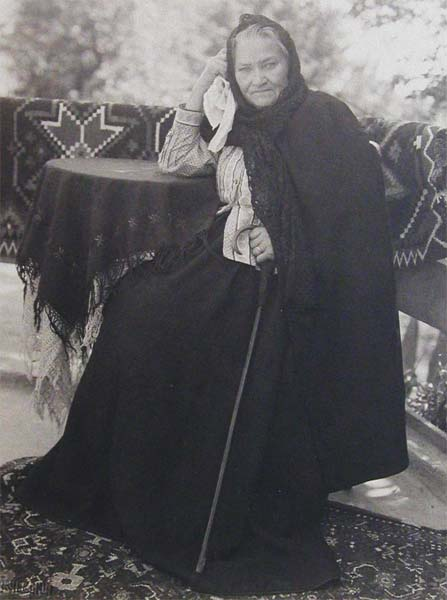
\includegraphics[width=0.98\linewidth]{chast-colebanie-osnov/nachalo/matvienko.jpg}

\textit{На снимке: Феодосия Матвеенкова.}
\end{center}

Между тем в подземелье повалили любопытствующие. Ребятня вытащила несколько черепов, катала по земли – кстати, когда в 1970-х строили крематорий на Байковом и разрушили часть погребений, тоже появились дети, игравшие черепами в футбол.

В пещеру на Ломаковской лазали все кому ни лень, а потом местным это надоело. Каманин пишет, что после заявления в комендатуру жителей усадеб, близких к пещерам, прислали рабочих с лопатами, и те засыпали вход.

По словам Матвеенковой, среди наплыва людей в пещеры был некий профессор Иванов со студентами. Каманин припоминает, что в 80-90 годах 19 века в газете «Киевлянин» проскользнула заметка о том, что неутомимый исследователь древностей и пещер профессор Владимир Бонифатьевич Антонович посетил Зверинецкие пещеры и обнаружил пояса и четки. И что обстоятельному изучению пещер профессором помешало Инженерное ведомство, ибо пещеры находились на территории Зверинецкой крепости. 

Думаю, память подвела Каманина. В 1895 году Антонович выпустил свою знаменитую «Археологическую карту Киевской губернии»\cite{antonovich01}, где по Зверинцу написано ровно следующее:

\begin{quotation}
Предместье Зверинец. Вблизи церкви в 1888 году открыта пещера, служившая вероятно монастырскою усыпальницей. Она представляла широкий коридор в 32 саженя\footnote{68,3 метров.} длиною; в стенах его сделано 48 нишей и в каждой лежало по 2 скелета, у них найдены 2 серебряные креста, несколько бронзовых, кресты плетеные из ремешков, скуфия и остатки обуви.

Киевское слово 1888 г. № 509. Коллекция Хойновского.
\end{quotation}

Как видим, Антонович использует в качестве источника статью из «Киевского слова». Никаких планов пещеры, как кое-кто пишет, в «Археологической карте» нет. Только эта коротенькая заметка.

%Думаю, дело было просто. Когда открыли пещеры, оттуда вытащили всё ценное, что успели – до того, как рабочие пришли и закопали вход. 

Указанные в ней предметы попали в коллекцию археолога Иосифа Адамовича Хойновского (сочинителя очерка «Раскопки великокняжеского двора древнего града Киева, произведенные весной 1892 года»).

В редакции «Киевлянина», где Каманин пытался разы\-скать нужный номер, никто про заметку о пещерах не помнил. А статья в самом деле была, в номере за 12 октября 1888 года – к сожалению, я не смог ее достать. Знаю кратко, что речь шла о провале в земле, возникшем при раскопке склона, где местные брали глину. И дескать открылись «громадные подземные пещеры, напоминающие лаврские».

Каманин много лет сотрудничал с Антоновичем в разных областях, например в создании историко-топографи\-ческих словарей. Но Антонович умер прежде, нежели Каманин начал работу над книгой про Зверинецкие пещеры. Иначе Каманин узнал бы сведения у самого профессора, не прибегая к поискам статьи.

Вы заметили, что Матвеенкова говорила о весне 1882-\-83 годов, а сведения Антоновича относятся к 1888-му?

Николай Петров тоже это заметил в своей брошюре, и нашел другие публикации про пещеры за 1888 год. Он решил, что старенькая Матвеенкова перепутала годы, да вот упустил – Матвеенкова говорила о весне, а вход в пещеры в 1888 году открылся осенью. Матвеенкова перепутала и год, и пору года? Или это два разных «открытия» пещер в северной части Зверинецкого холма?

Петров приводит заметку из «Киевского слова» за 15 октября 1888 года (№ 509) – на которую ссылался Антонович. Петров полагал, что корреспондентом «Слова» был художник Димитрий Зайченко, хотя, даже если не принимать во внимание разницу лет, описания посещения пещеры отличны. В 1882-м лезут двое, в 1888-м трое. Зайченко сам, в полдень, нашел провал, а в 1888-м – сочинителю заметки в 4 часа дня рассказывает о провале знакомый. Судите впрочем сами:

\begin{quotation}
В 4 часа пополудни, 13 октября, до меня дошло известие, что на Зверинце, недалеко от того места, где я живу, открыта новая пещера, и в ней покоятся кости мертвецов. Кем открыта эта пещера и при каких обстоятельствах, никто мне сообщить не мог.

Ко мне подошел живущий на Зверинце К-н и предложил мне идти с ним. Втроем, я, г. К-н и еще один незнакомый мне мужчина, решились спуститься в пещеру, конечно, зажегши предварительно свечи...

При свете свечей, по бокам этой пещеры, в стенах ея с двух сторон мы увидели полукруглые углубленные могилы, где лежали груды человеческих костей, и по два черепа в каждой могиле, причем в некоторых могилах отчетливо видны два человеческих скелета, положенных головой внутрь, а ногами к пещере, так что безошибочно можно заключить,что в каждой могиле находится по два человека.

Пещера оканчивается вертикальной стеной, и в ней находится такая же углубленная могила с двумя человеческими скелетами. Во всей пещере мы насчитали 48 могил, и считая в каждой могиле по два человека, всего будет похороненных 96 человек.

Вся пещера имеет длины приблизительно 96 аршин\footnote{68,28 метров.}. В пещере этой мы нашли два красных кирпича, шириной примерно 1,5 аршина\footnote{1,07 метра.} и толщиной 1 вершок\footnote{4,5 сантиметра.} (длина неизвестная, так как кирпич по длине сломан), уже довольно выветренных, так что рассыпаются, и формой совершенно не похожих на кирпич теперешних образцов, а также нашли кусочки ветхой кожи от обуви.

Больше ничего не оказалось; гробов и следа нет; но в толпе ходят слухи, что будто бы какие-то люди осматривали пещеру раньше и на костях видели уже истлевшее духовное облачение и нашли золотой крестик. 

Болтают также, что будто бы лет 80 тому назад здесь случился обвал и завалил покоющихся здесь. Но это совершенно неправильно.
\end{quotation}

Матвеенкова в 1882 году видела ниши только в правой стене, гробы (хотя бы истлевшие), обитую железом дверь, и трупы головами к выходу из камер. В 1888-м у корреспондента – ниши по обе стороны коридора, никаких гробов и двери, трупы ногами к выходу.

Кажется, в 1882-83 и 1888 году открывались входы в две разные части пещерного комплекса, возможно даже не соединенные между собой.

Петров пишет\footnote{Ссылаясь на «Киевское слово» от 8 ноября 1888, номер 242.}, что прочитав заметку в «Киевском слове», 16 октября 1888 года к пещерам отправились профессор университета Св. Владимира Адриан Викторович Прахов
\footnote{Руководитель росписи Владимирского собора и реставрации Кирилловской церкви.}, художник Т. А. Сведомский да исследователь древностей В. И. Гошкевич.

\begin{quotation}
Профессор Прахов остался на страже у входа в пещеры, а остальные двое отправились в самую пещеру, захватив с собой длинный шнур для сигнализации и для того, чтобы не заблудиться в лабиринте пещерных ходов.

По описанию г. Гошкевича, влево от найденной пещеры виднелась другая пещера, устье которой выходило в нескольких шагах от первого отверстия. Вся длина пещеры около 30 метров. 

К сожалению, за 4 дня со времени ея открытия успело перебывать множество «варваров», окончательно нарушивших первоначальное положение скелетов, так что теперь весьма трудно его определить.

Разрушительная работа велась, по-видимому, таким образом, что не только в самых пещерах все предметы разбросаны, но и содержимое ниш выгребено в пещерный коридор.

В самой пещере Сведомский и Гошкевич встретились с каким-то субъектом, предлагавшим им свои услуги по отысканию могильных предметов.

Но не успели исследователи осмотреть пещеру надлежащим образом, как получили от профессора Прахова предупредительную записочку об угрожаемой им опасности от обвала пещеры, так как над пещерами, в которых находились исследователи, собралась громадная толпа любопытствующих зрителей.

Исследователи благополучно выбрались из пещеры и уже когда двинулись в обратный путь домой, то встретили полицейского, спешившего к месту скопления толпы.
\end{quotation}

Сравним числа. Тут длина пещеры – около 30 метров. А в заметке от 15 октября 1888 года – как мы помним, около 68 метров. Разница слишком велика, чтобы быть ошибкой. В ту ли самую пещеру лазали Гошкевич со Сведомским?

Киевское Военное ведомство отправило в пещеру, посещенную последними, инженера Червинова 2-го. Гошкевич в начале ноября сообщал:

\begin{quotation}
Военным инженером Червиновым 2-м совершена на днях экскурсия в новооткрытую на Зверинце пещеру. Исследование затруднено теперь еще больше по причине происшедшаго в последние дни внутреннего обвала.

Червинову удалось начертить правильный план этого подземелья, с обозначением на нем всех погребальных ниш. Количество их определено им в 36. Так как в каждой нише находится по два скелета (в одной, впрочем, найдено нами 3 скелета), то число всех покойников, погребенных в этой усыпальнице, должно быть не менее 72. Кроме значительного количества лоскутков кожи, других предметов при скелетах г. Червиновым не найдено.

План пещеры, вместе с одним из лучше сохранившихся черепов, будет отправлен в С.-Пе\-тербургский Археологический Институт\footnote{Петров добавляет, что на деле отправили в Императорскую Археологическую Комиссию, а та в 1891 году переслала в Церковно-Археологическое общество при Киевской Духовной Академии, для музея, сандалию из Зверинецких пещер.}.
\end{quotation}

36 ниш против 48 из заметки за 15 октября. Спишем на обвал, или – таки другая пещера?

Затем Зверинецкие пещеры выпадают из поля зрения ученых и общественности до 1911 года,  когда снова провалилась земля и открылось два новых входа. Каманин пишет, что 30 лет эти пещеры «находились без охраны», Эртель говорит про 20 лет – однако если в 1911 году пещеры вновь «открылись», значит, старые входы были завалены (нет и точных сведений об их месте). О каких же 20 или 30 годах разорения пещер идет речь? Вход 1882-го, по сведениям Каманина, закопали власти. Судьба входа 1888 года теряется в истории.

%Тогда-то и началось масштабное изучение пещеры Эртелем при содействии князя Жевахова.

Каманин (совмещая, как я считаю, два обнаружения пещер 1882 и 1888 годов в одно событие) полагал, что Матвеенкова попадала в какую-то другую пещеру (или часть), не ту, где рыл Эртель и примкнувший к нему позже Вельмин. Так можно судить по описаниям, оставленным последним, и показаниям самой Матвеенковой, которая уже при Эртеле, когда ее повели под землю, не узнала пещеру. Найденные тридцать лет назад ею пещеры – «это не те пещеры, которые теперь раскопаны – это другие пещеры, до которых еще не докопались. Надо копать в правую сторону, более под мою усадьбу».

По Сети бродят сведения без источника, что георадиолокация показывает еще около километра неизвестных пещер. В одном из коридоров Зверинецких пещер – «Погребальной улице» – есть завал, где через десять метров прощупывается пустота – и вот что за этим завалом, пока неведомо. Вероятно это те самые исследования, которые производились Институтом прикладных проблем экологии, геофизики и геохимии в 2001 году, из коих мне известно следующее – в ботсаду и по Мичурина 10, 12 и 14\footnote{Мичурина 10 – это не Ломаковская 10, нумерация сильно сдвинулась. У меня нет уточняющих данных, но как я понимаю, участок ботсада с пустотами примыкает к упомянутым усадьбам. В ботсаду там растут огромные акации.} показали на площади 65x115 метров наличие там «аномальных зон», которые трактовали как подземные пустоты. Проверяли ли дальше на юг, номер 8 и местность Собачку, я не знаю. Но от жителей усадьбы номер восемь я слышал только историю о живущем на чердаке домовом, а про пещеры ничего не слышал, равно как не замечал их на Собачке, прожив рядом добрые двадцать лет.

Эртель во время раскопок 1912 года увидел, что от Зверинецких пещер в сторону Ионинского монастыря идет подземный ход, и предположил, что всё пространство между монастырем и Зверинецкими пещерами изрыто ходами, но там находился Зверинецкий форт, под который копать было невозможно\footnote{К слову, когда в ботсадовском Розарии (лежит в пределах бывшей крепости) вместо нынешнего центрального бассейна было озеро с земляными берегами и фонтанами (по плану ландшафтного архитектора Рубцова), вода просто уходила в какие-то подземные пустоты. Даже когда в 1970-х забетонировали дно и построили каменные бортики, вода продолжала уходить.}. Эртель также нашел провалы в несколько отдаленной от раскопок усадьбе зубного лекаря В. Шмигельского и подумал, что под ними тоже части пещерной сети. К слову, по северной и западной возвышенной части горы Эртель заметил древний вал и сопоставил его с упоминаемым в летописи Красным двором Всеволода Ярославича. Там где сейчас в ботсаду воссоздан «Красный двор» в самом деле кромка склона издревле несет следы земляных работ, а под тамошним обрывом я находил плинфу – древнерусский кирпич. Мыс с обрывом именуется «мыс Чайка». Название, по одной версии, от бывшей тут дачи профессора-уролога Андроника Архиповича Чайки, а по другой версии - от фамилии капитана красноармейcкой батареи, стоявшей здесь во время Великой Отечественной войны.

В 11 номере «Киевской мысли» за 1913 проскользнули упоминания о втором ярусе пещер (их же повторил в виде предположения Шероцкий в газете «Рада», №2 за 1913 год), над открытыми, и о провалах возле Ионинского монастыря\footnote{Около монастырской ограды археолог Стеллецкий позже нашел некий подземный лабиринт, и выразил мысль что всё это часть единой со Зверинецкими пещерами подземной системы ходов.}, и что один такой провал забирает всю весеннюю воду. В 29 номере «Киевлянина» за 1913 тоже есть про второй ярус пещер, причем если Шероцкий полагал что он находится над уже раскопанными ходами, в «Киевлянине» речь идет о нижележащем этаже:

\begin{quotation}
Недавно в галерее, соединявшей старый и новый выходы из пещер, приблизительно в средней ее части обнаружена небольшая лазейка, за которой замечена круглой формы небольшая комната. В ней имеются ясные признаки заваленного хода – спуска. Возможно, что это спуск во второй ярус пещер, о котором местное население давно говорит и куда некоторые местные старожилы уже проникали несколько лет тому назад и по их описанию эти пещеры имеют иной вид, нежели открытие пещеры. Там были сравнительно большие комнаты, находились части облачений, ручные кресты и другие предметы.

Рассказы о существовании второго нижнего ряда галерей и пещеры находят себе некоторое подтверждение в существовании провалов на поверхности всей площади, направление которых не совпадает с открытыми уже галереями, но почти тождественно с направлением пещер, о которых говорят местные жители. Между тем на этой площади, как мы слышали, предполагается постройка больших воинских казарм.
\end{quotation}

...Как известно, поныне раскопан только один ярус.

В 1911 году набожный князь Владимир Жевахов (будущий Иоасаф, архиепископ Могилевский) взял в аренду на 6 лет участок земли в 350 квадратных сажень (746,8 кв. метров) с новооткрытыми пещерами и организовал там раскопки. Позже Жевахов ходатайствовал о передаче этого участка и окрестностей духовному ведомству, но военное ведомство отказало, ибо собиралось строить там казармы для частей Киевского гарнизона, и посоветовало арендовать взамен соседнюю частную усадьбу.

\begin{center}
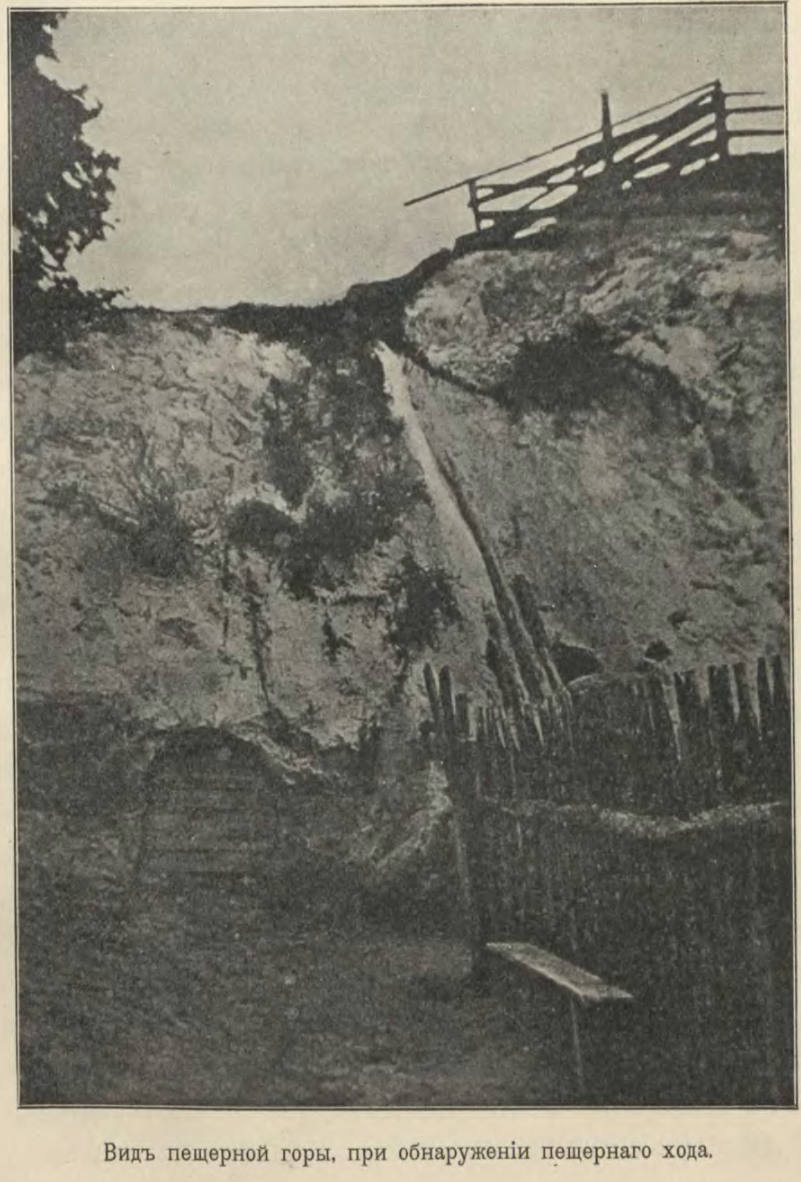
\includegraphics[width=0.90\linewidth]{chast-colebanie-osnov/nachalo/zverp-02.jpg}

\textit{Снимок 1911 года.}
\end{center}

\newpage

Петров осторожно пишет:

\begin{quotation}
О новооткрытых пещерах узнал проживавший тогда в Киеве князь Вл. Д. Жевахов, тот самый, который, вместе с братом своим Николаем, так сильно хлопотал об открытии нетленных мощей и канонизации своего родственника по женской линии, святителя Иоасафа Горленка, епископа Белгородского.

Князь задумал открыть Зверинецкие пещеры не столько как памятник глубокой древности, сколько как народную святыню, и сделать их доступными для народного поклонения и чествования. Этою религиозною целию забот князя Жевахова нужно объяснить то обстоятельство, что он обратился за разрешением работ не к Императорской Археологической Комиссии, ведающей все находки и раскопки древностей, а к духовному начальству, хотя не пренебрегал совершенно и научными интересами. Осенью 1911 года он взял в аренду у Инженерного ведомства тот участок земли, на котором находились Зверинецкие пещеры, и попросил благословение на открытие пещер у Киевского Митрополита Флавиана, которому князь сообщил о пещерах письмом. Наместник Киевопечерской лавры архимандрит Амвросий предложил заняться раскопкою этих пещер секретарю Киевского Общества Взаимного Кредита А. Д. Эртелю.
\end{quotation}

Раскопки начались только в июле 1912, поначалу даже без Эртеля – тот был занят в Китаевских пещерах, полагая в последних начало древнего Киева.

Копия рапорта Киевского полицмейстера от 28 июля 1912 года за № 9951 на имя Киевского Губернатора.

\begin{quotation}
На арендуемом князем Жеваховым от инженерного ведомства участке земли, находящемся сзади № 10 по Ломаковской улице производится богомольцами-охотниками\footnote{Т.е. желающими, добровольцами.} под руководством рабочаго крестьянина Семена Гончарова раскопки в целях открытия древних пещер-усыпальниц. 

%В настоящее время под горой Печерскаго укрепления открыт вход в пещеру, оказавшуюся в измерении 3 1/2 аршина\footnote{2,5 метра.} в квадрате, а из нея в глубь горы имеется ход в виде корридора шириною 2 арш. 2 вершк.\footnote{1,48 метра.}, вышиной 1 арш. 2 вер.\footnote{0,8 метра.} и длиною 41 аршин\footnote{29,2 метра.}, в нем обнаружено 32 места, где, повидимому, находились гробы с телами, на что указывают найденные остатки человеческих костей.

В настоящее время под горой Печерскаго укрепления открыт вход в пещеру, оказавшуюся в измерении 3 1/2 аршина в квадрате, а из нея в глубь горы имеется ход в виде корридора шириною 2 арш. 2 вершк., вышиной 1 арш. 2 вер. и длиною 41 аршин\footnote{2,5 метра в квадрате, 1,48 метра ширина, 0,8 метра высота. 29,2 метра длина.}, в нем обнаружено 32 места, где, повидимому, находились гробы с телами, на что указывают найденные остатки человеческих костей.

Раскопками заведует игумен Свято-Троицко\-го монастыря о. Валентин. 

Об этом доношу Вашему Превосходительству. Подлинное за надлежащими подписями.

С подлинным верно: Правитель Канцелярии Киевскаго Губернатора (подпись)

Сверял: Помощник Правителя (подпись)\end{quotation}

Мысленно потираю руки – обсудим! Вот у нас появился адрес пещер – участок земли позади усадьбы номер 10. Как мы знаем, на самой Ломаковской, 10 жила Матвеенкова. Ломаковская теперь называется Мичурина, и 10-й номер по Мичурина это, на 2016 год, частный дом, стоящий под горкой на той же стороне улицы, где и Зверинецкие пещеры, которые ныне имеют адрес Мичурина, 20-22 (в 1998-м: 18-22). От номера 10 до 20 около 150 метров. Значит, старая и новая нумерация не совпадают. Сравним теперь числа «от Матвеенковой» 1882 года, 1888-го и 1912-го.

У Матвеенковой – 50 гробов в отдельных пещерках по правой стене, по два тела в каждой могиле. И значит, 50 ниш в одной только стене. А другая, стало быть, без ниш.

1888 год, в первой заметке от неизвестного корреспондента – «по бокам пещеры» 48 могил с двойными погребениями. В одной из последующих заметок, уже в пещере, где побывали Прахов, Сведомский, Гошкевич и Червинов 2-й – 48 могил, при этом неясно, по одной стороне коридора или обеим.

Наконец 1912 год, первые раскопки – 32 ниши, и согласно позднейшим планам пещер – в каждом коридоре ниши были по обе стороны.

Затем раскопками стал руководить Эртель, поставив дело на научную основу. Кроме прочего он составил план расчищенного им участка пещер, несколько позже другой план начертил В. В. Кузнецов, сотрудник покойного к тому времени археолога Д. В. Милеева.

Перед разбором планов опишу рельеф местности. Северо-восточный, клиноподобный угол Зверинецкого холма. Сверху вниз – крутой склон (со входом в пещеру у его подножия), терраса с Ломаковской улицей, затем более пологий склон. Вдоль улицы, с течением времени, верхний крутой склон террасировался для разбивки там садов и огородов частного сектора.

\begin{center}
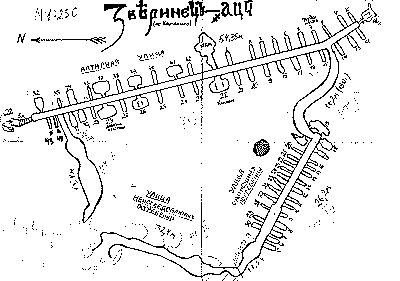
\includegraphics[width=0.90\linewidth]{chast-colebanie-osnov/nachalo/zverp-plan01.jpg}

\textit{Один из планов пещер, открытых в 1911 – еще не прорыт соединительный коридор для удобства паломников.}
\end{center}

\newpage
\vspace*{\fill}

\begin{center}
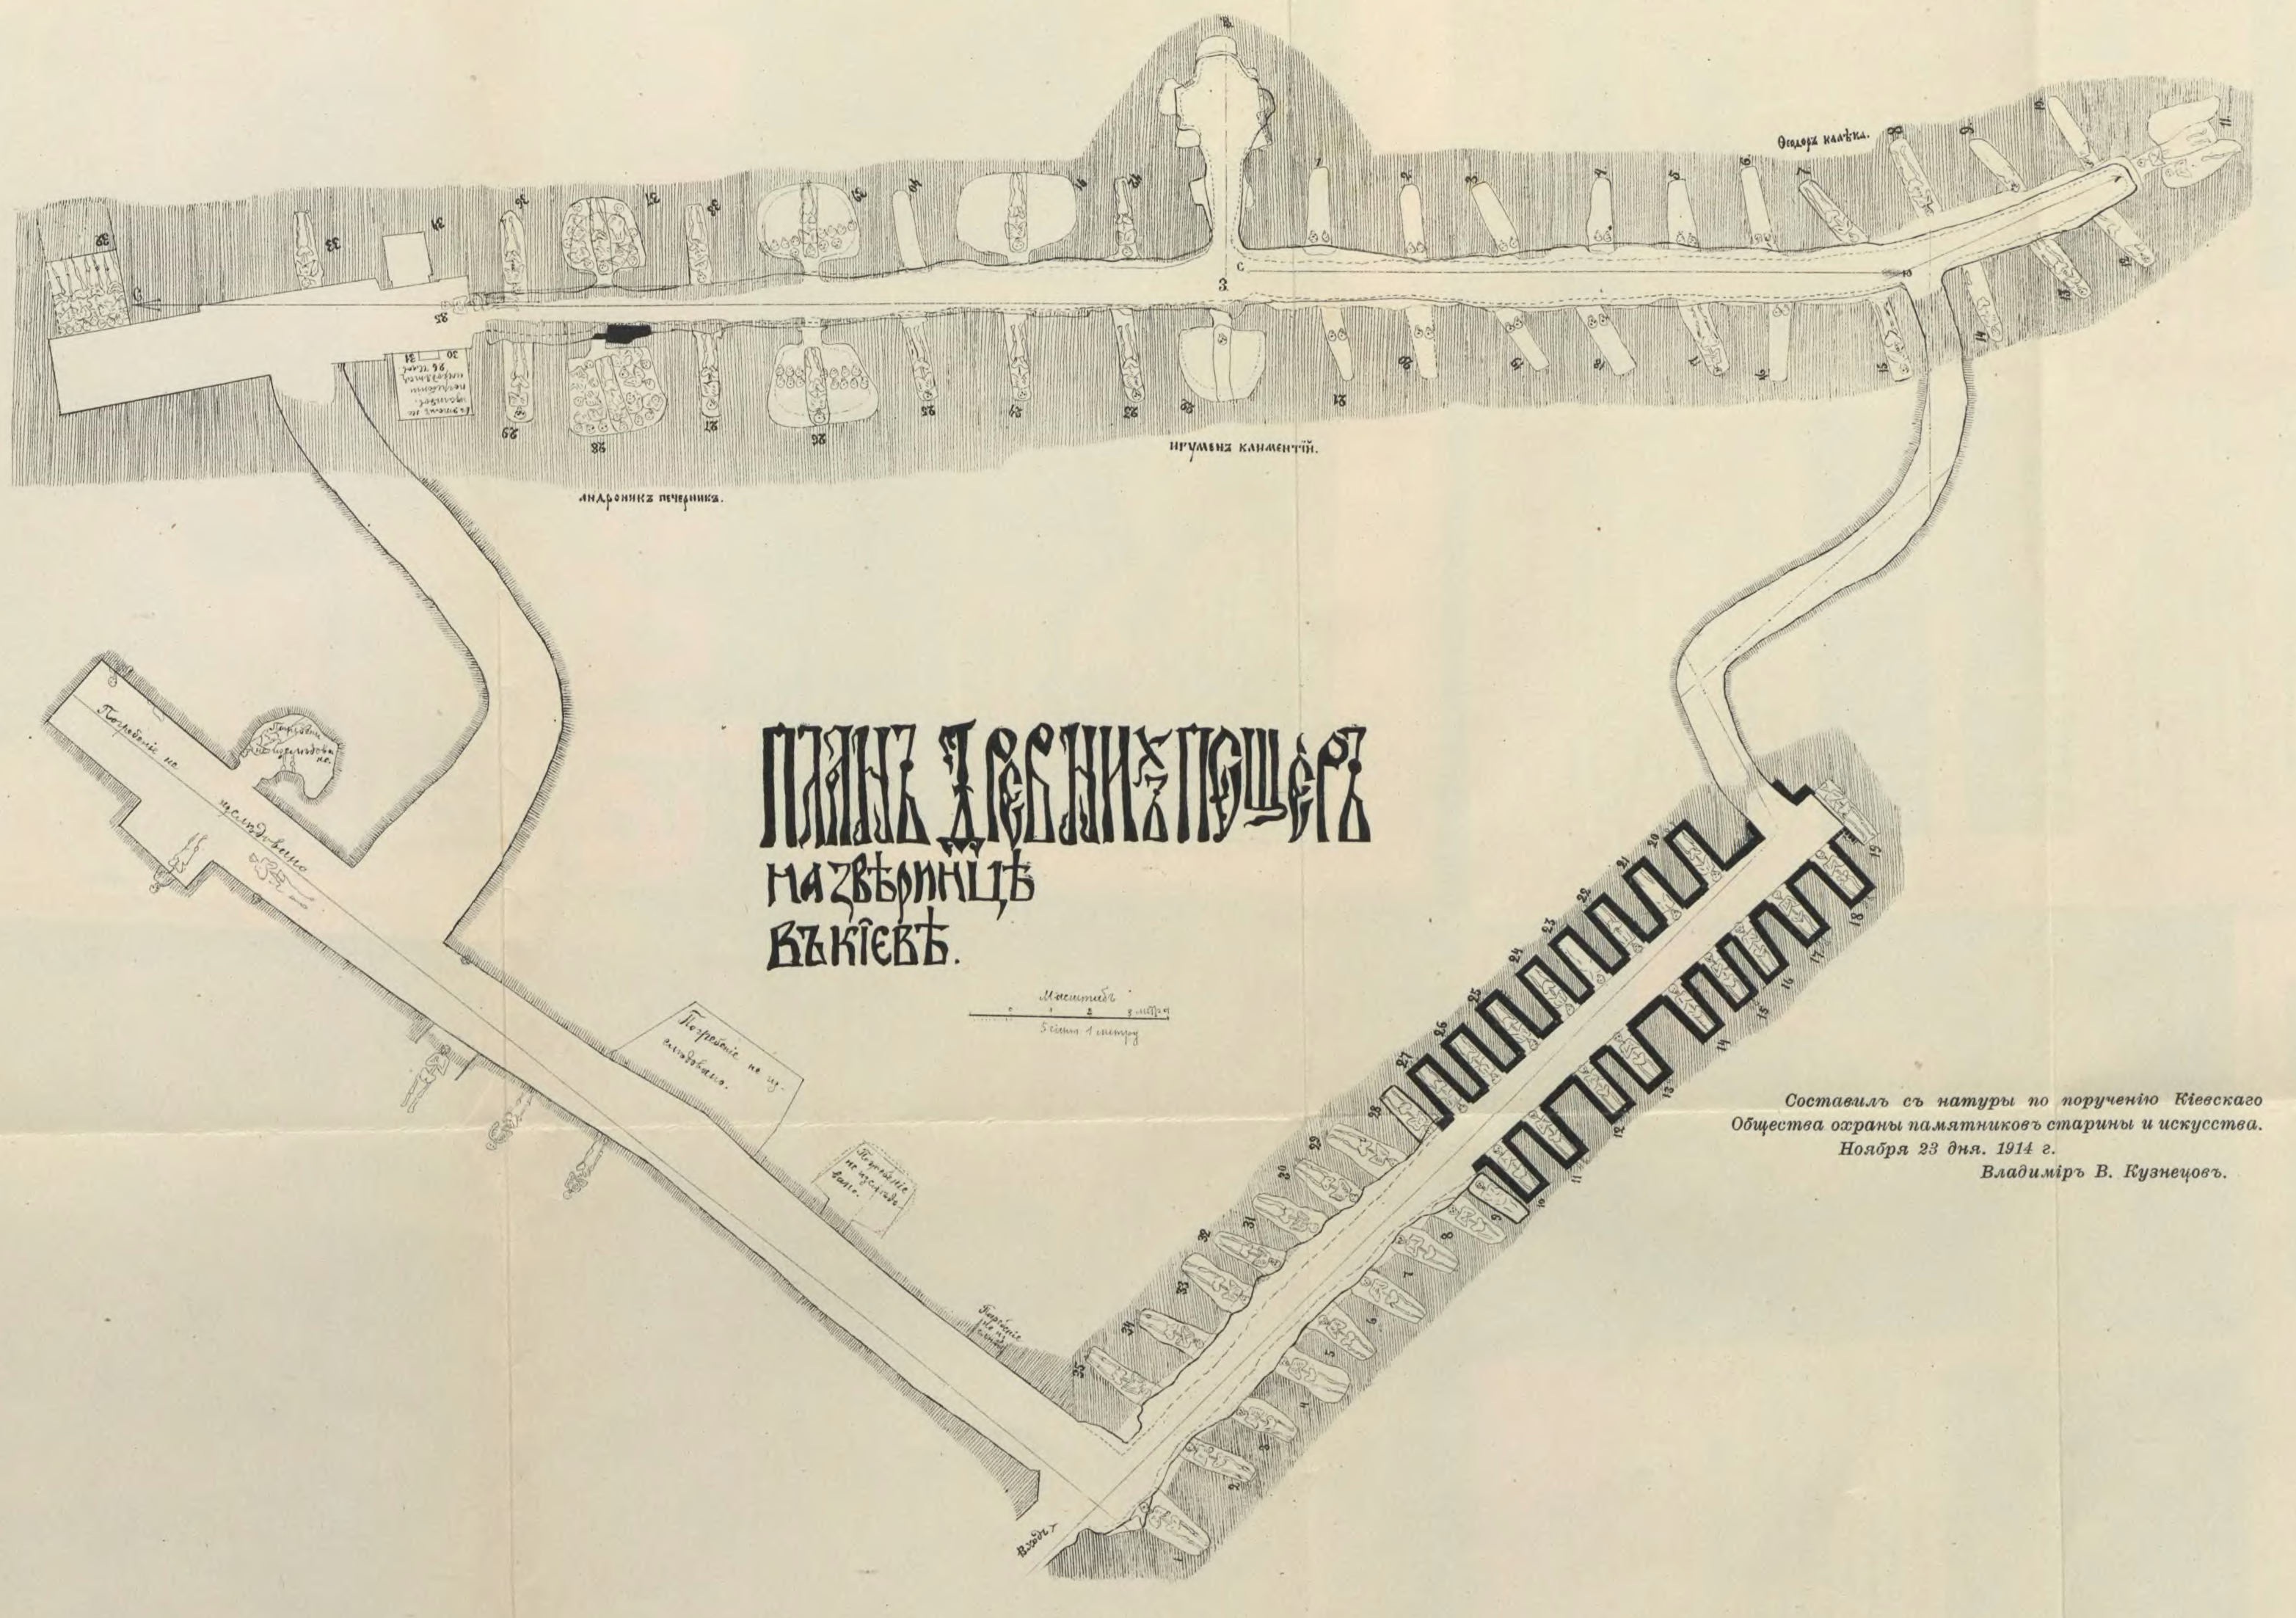
\includegraphics[width=\linewidth]{chast-colebanie-osnov/nachalo/zverp-plan02.jpg}

\textit{План Кузнецова. Современный вход – слева сверху.}
\end{center}

\begin{center}
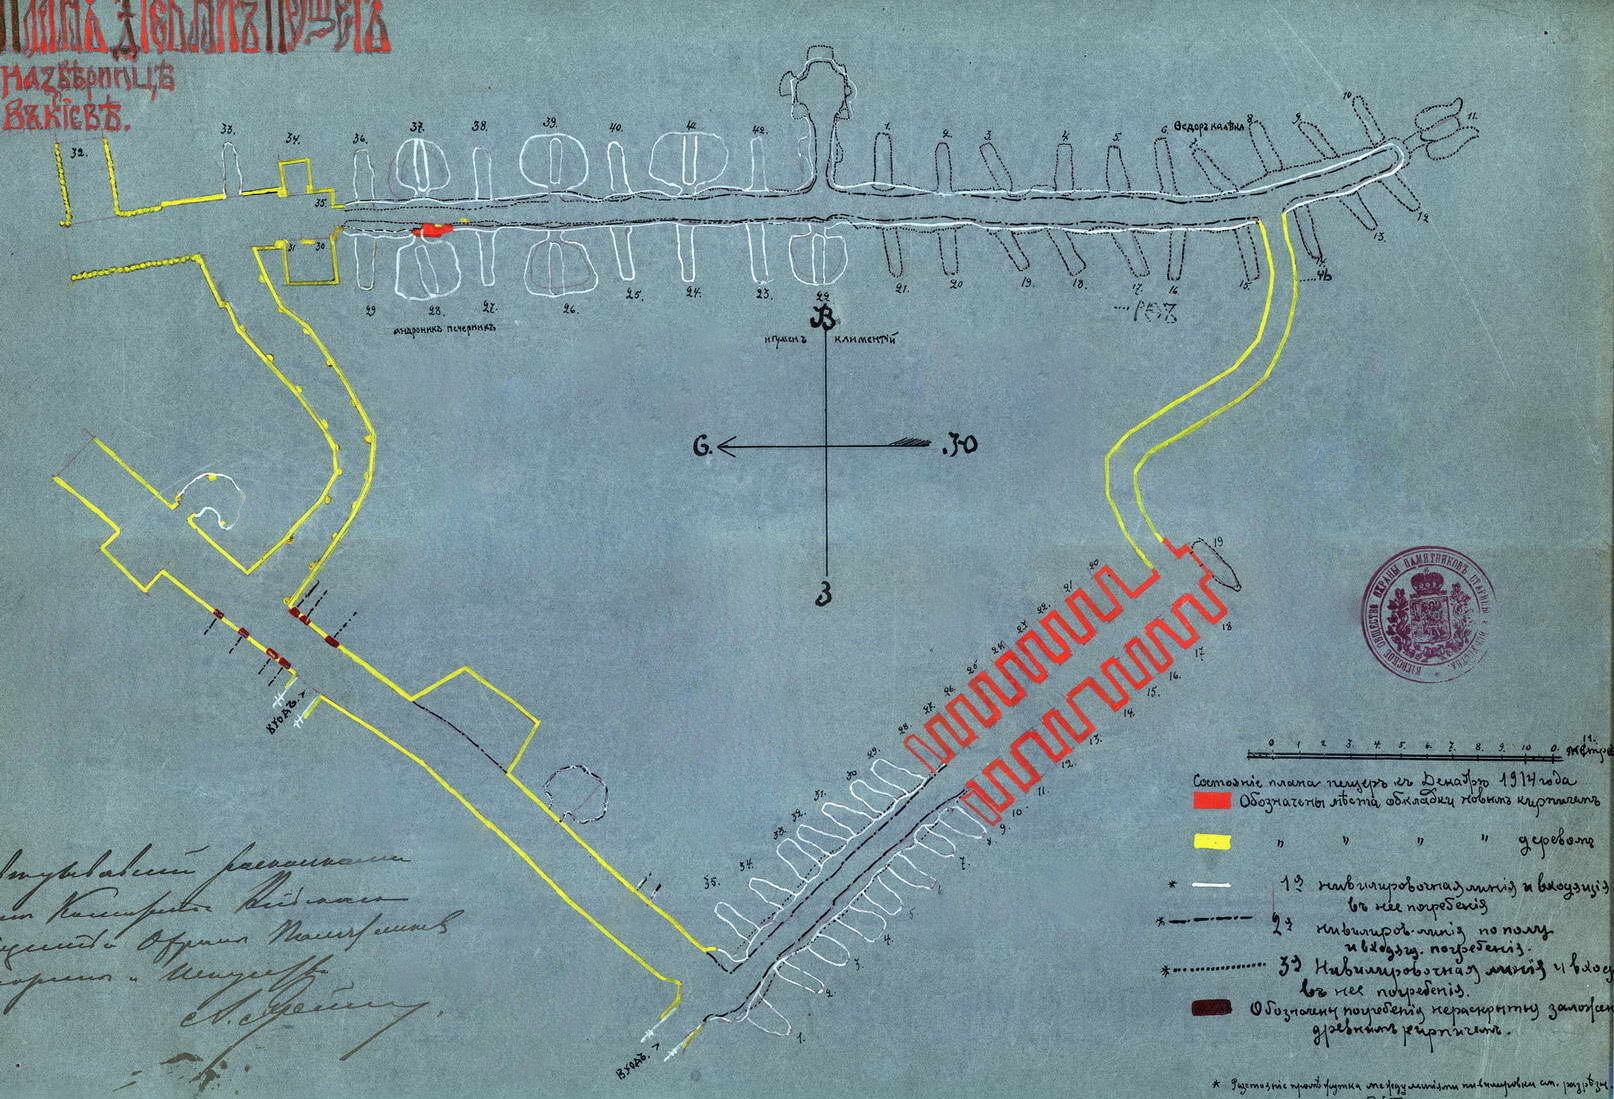
\includegraphics[width=\linewidth]{chast-colebanie-osnov/nachalo/1914-ertel.jpg}

\textit{1914. План с подписью Эртеля.}
\end{center}

\vspace*{\fill}
\newpage

Пять коридоров («улиц»), взаимное расположение которых образует треугольник. Разница между планами – пара лет, однако на втором видно, что прорыли коридор, соединивший северные части двух улиц.

Где находился изначальный вход 1911 года, не вполне ясно, однако на плане Кузнецова вход – посередине внизу плана, и на другом плане 1914 года появляется второй вход едва не на месте погребений. Современный же, 21 века вход – в верхнем левом углу.

%Очевидно, что подземелье было вырыто по начертанному ранее проекту, и в ходе работ использовались какие-то измерительные средства, позволившие придерживаться начального чертежа.

Обмеры коридоров, по Кузнецову, таковы. Правый от тогдашнего входа («улица одиночных погребений») – длина 26,20 метров (13 сажень), на одной стороне 18 ниш, на другой 16, одна в тупике, всего 35, погребения одиночные. Левый («улица неисследованных погребений») – 32,40 метра (19 сажень). Поперечный коридор («алтарная улица») – 54,35 метра (27 сажень), по стенам расположены комнаты с массовыми погребениями (останки более двух людей в одной келье), и около трех десятков двойных (скелеты лежали друг на друге) и одиночных погребений.

Говоря о кельях, которых на Алтарной улице насчитали три, Каманин сообщает, что «высота всех келлий общая с высотой пещер, от 1,80 до 2 метров». Пещеры, куда лазала Матвеенкова, имели высоту 2,1 метра.

Но вот газета «Киевлянин» в № 55 за 24 февраля 1913 года поместила заметку про доклад Эртеля и Каманина в феврале 1913 года на заседании Исторического общества Нестора-летописца. Выдержки оттуда, касаемо доклада Эртеля:

\begin{quotation}
На первых порах при зверинецких раскопках пришлось преодолеть некоторые затруднения: пещеры привлекли огромные массы паломников со всех концов Руси; своим любопытством они мешали работам, которые и без того требовали большого внимания и осмотрительности: возможен был обвал и за рабочими приходилось тщательно наблюдать.

Все это осложнялось еще спором о казармах, которые предполагалось строить на месте производства работ, по раскопкам. Сейчас раскопки далеко еще не закончены, но в некоторых местах подошли уже к границам частных усадеб.

Пока отрыты несколько низких (в них нельзя выпрямиться) длинных галерей со множеством усыпальниц, из которых большинство разрушено.
\end{quotation}

А почему Каманин в своей книге пишет о высоких потолках? Где же эти галереи, в которых нельзя выпрямиться? Читаем «Киевлянина» дальше:

\begin{quotation}
Кирпич, найденный здесь, относится к XI и позднейшим векам. Встречаются кирпичи, бывшие, очевидно, уже в употреблении и принесенные сюда из других построек. 

В конце одного хода обнаружены несколько скелетов, расположение которых наводит на мысль о какой-то драме, быть может, времен татарщины.

В центре открытой системы галерей (система незаконченная, неясная, что заставляет предполагать существование 2-го яруса подземных ходов) находится низкая четырехугольная камера, с нишами в северной и восточной стенах, где, предполагает докладчик, находились жертвенник и престол этой подземной церкви. вмещавшей не более шести человек.
\end{quotation}

Заметим предположение о втором ярусе пещер, краткие сведения о «драме», и указание на низкую камеру с жертвенником. Это же помещение по обмерам из книги Каманина становится если не просторнее, то по крайней мере несколько выше – два метра.

Посмотрим на выполненный Кузнецовым план Алтарной улицы в разрезе, 1914 года – все обмеры указаны в сажнях, а сажень это примерно 2,1 метра. Вид с востока:

\newpage

\vspace*{\fill}

\begin{center}
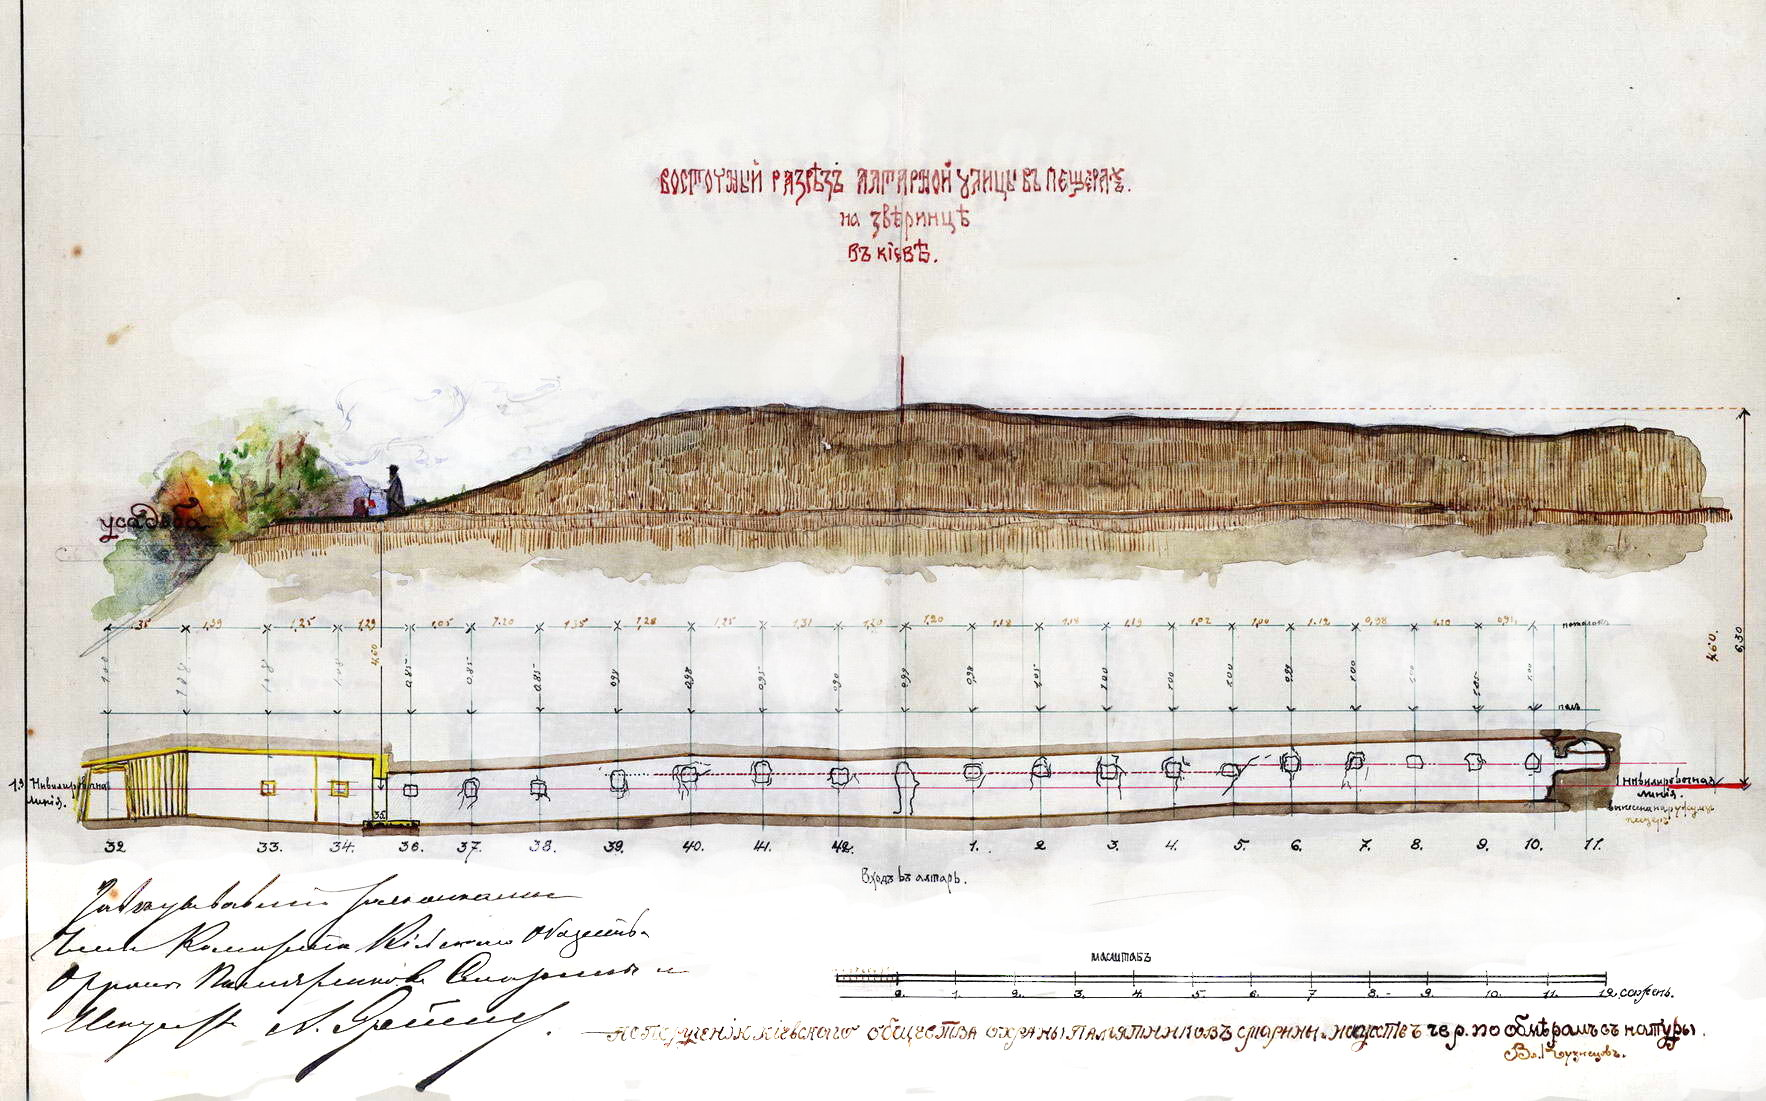
\includegraphics[width=\linewidth]{chast-colebanie-osnov/nachalo/1914-01.jpg}
\end{center}

\vspace*{\fill}

Над коридором изображена шкала, где для каждого участка по оси X отмечена его длина, а по оси Y – высота потолка.

Посередке обозначен «Вход в алтарь». Какая высота потолка? 0,99 сажени – это таки около двух метров.

Со времени доклада Эртеля потолок подрос? Судя по данным высот с этого же «разрезного» плана, нигде в Алтарной улице не нужно идти пригнувшись.

Что кстати еще полезного можно узнать из плана? Видите две фигуры на пригорке – черную и в красной шапке? Эти люди пробурили в коридор шахточку, и высота ее составила 4,60 сажни, это 9,66 метра. Ниши в коридоре пронумерованы до 42.

Познакомимся с разрезом «Второй улицы» («одиночных погребений») с запада, причем на плане отмечены только ниши, находящиеся по правую руку, если смотреть от обозначенного на нем входа (тоже справа). Всего же ниш – 35.

Масштаб указан уже не в сажнях, а в метрах – вероятно, обмеры тоже в метрах.

\begin{center}
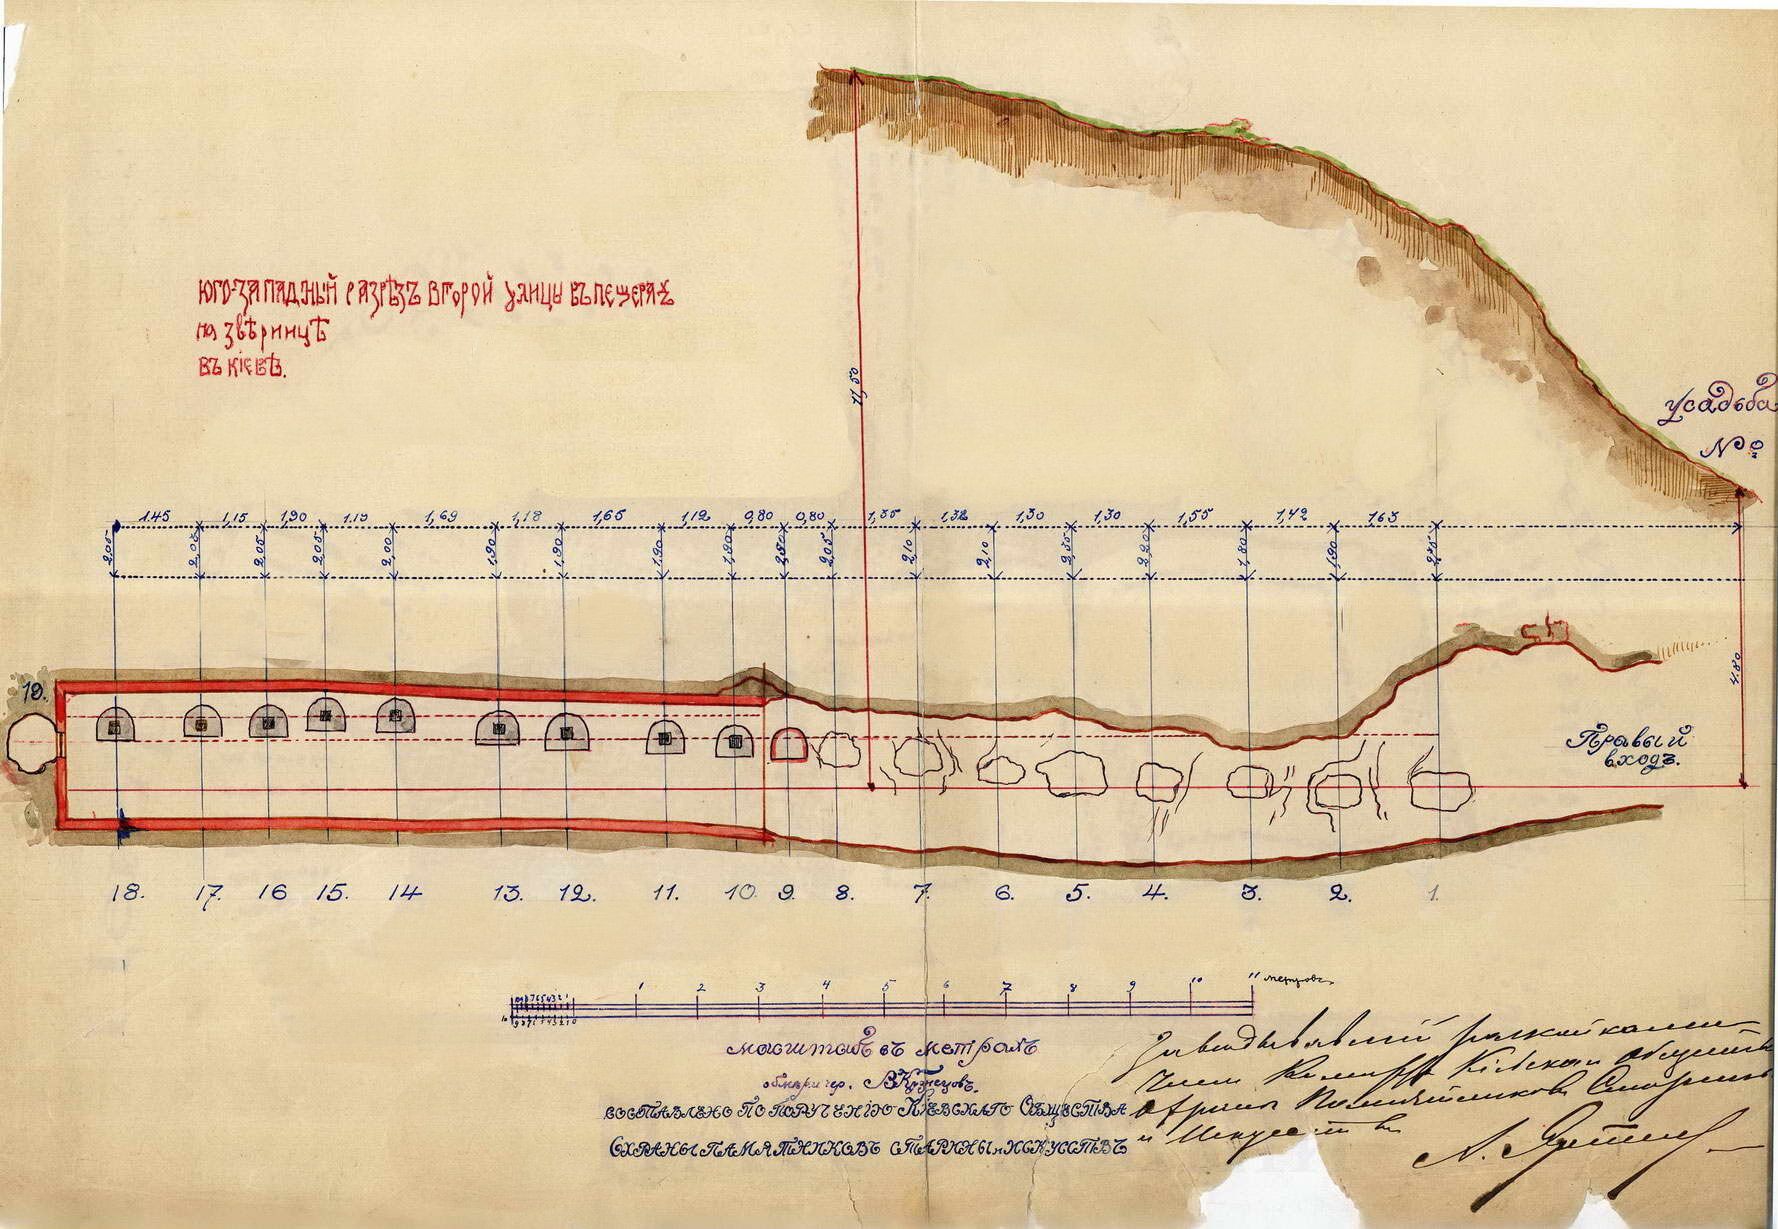
\includegraphics[width=\linewidth]{chast-colebanie-osnov/nachalo/1914-02.jpg}
\end{center}

То, что числа выражают метры, подтверждается указанной глубиной залегания коридора – 11,50 от поверхности. Если Алтарная улица лежала в 9,66 метрах, то 11,50 – сопоставимая величина, ведь если бы 11,50 было в сажнях, это даст нам глубину более 20 метров. А поскольку оба коридора лежат примерно на одном уровне, значит, 11,50 – именно метры.

Может быть это низкий коридор, где нельзя разогнуться? Да вроде бы нет, один только участок 1,80 метра, остальные 1,90 и даже более 2 метров. 

А как же данные самого начала раскопок? Когда

\begin{quotation}
а из нея в глубь горы имеется ход в виде корридора шириною 2 арш. 2 вершк., вышиной 1 арш. 2 вер. и длиною 41 аршин, в нем обнаружено 32 места, где, по-видимому, находились гробы с телами
\end{quotation}

Здесь высота потолка – 0,8 метра, длина около 30-ти. 32 ниши против «официальных» 35 с плана Кузнецова. Будто тот же самый коридор, да вот только высота потолка снова стала много выше. 

Воистину чудесны киевские пещеры! 

Из подземного хода, где надо ползти на карачках, всего за пару лет образуется удобный для пешего хождения коридор.

Сам Эртель в книге 1913 года писал про «улицу одиночных погребений» следующее:

\begin{quotation}
Правый ход (А) ведет в длинный коридор, в котором по обе стороны расположены одиночные и двойные усыпальницы, к сожалению, все разрушенные и разграбленные. В них остались только разбросанные в беспорядке кости, часть которых, по-видимому, унесена или перенесена в другое место. Кости – плохой сохранности, и некоторые совершенно рассыпаются.

Усыпальницы расположены так густо, что промежутки между ними занимают не более полуаршина. Местами сохранились обломки почти совершенно истлевших деревянных досок (по-видимому дуб), но были ли тут гробы, определить с уверенностью нельзя.

Ход в общем широкий, но низкий, так что почти везде нужно идти согнувшись.
\end{quotation}

Низкий ход... Идти согнувшись... А согласно плану – средняя высота потолка около двух метров!

В докладе на заседании общества Нестора-Летописца говорилось, что останки, вид которых намекал на некую трагедию, лежали в конце коридора. Каманин же сообщает в книге, как свидетельство внезапной гибели людей, что часть скелетов, лежала на полу коридоров, и много ближе ко входу, в беспорядочном положении.

Как бы ни было, это можно толковать двояко – люди погибли и остались на месте смерти, либо же их останки переместили уже после, например при разграблении пещер.

Некоторые ниши-усыпальницы были заложены кирпичом (датированным 11 веком, однако вроде были и позднейшие). Эртель нашел также кирпичные плиты, похожие на части круглых колонн. Предметы из кожи – плетеные кресты, остатки обуви, а также поясов с названиями либо оттисками изображений христианских праздников (в прямоугольных рамках до трех сантиметров в ширину, около двух в высоту, видны распятие Христа, въезд его в Иерусалим на «жребяти осли», воскресение Лазаря, и тому подобное), несколько черепков.

\begin{center}
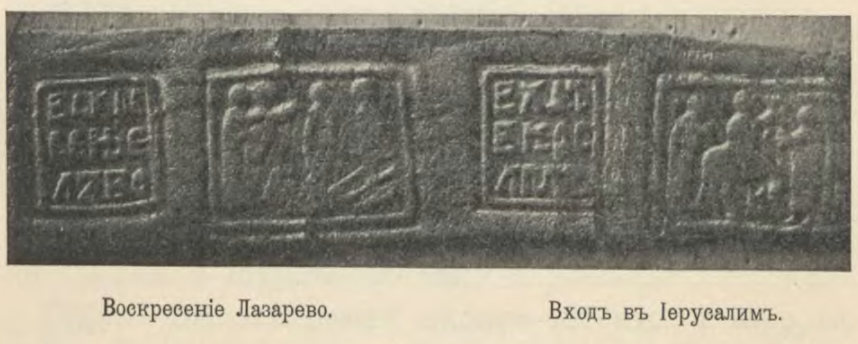
\includegraphics[width=\linewidth]{chast-colebanie-osnov/nachalo/poyasa.jpg}
\end{center}

%\begin{center}
%\includegraphics[width=\linewidth]{osn-kiev/poyasa02.jpg}
%\end{center}

По находкам Эртель судил, что подземный монастырь существовал в 12, 13 и 17 веках. Непрерывно или временами?

Описание пещер 1911 года открытия кажутся мне отличными от пещер открытия 1882 и 1888 годов, на что указывают хотя бы числа – длины коридоров и связанные с ними количество и виды захоронений (одиночные, двойные, массовые), наконец сведения о нишах только справа – у Матвеенковой.

%В статье про Зверинецкие пещеры из сборника «Звід пам'яток історії та культури України. Київ» 1999 года издания, где все местные подземелья смешали в одну кучу, упоминаются еще некие исследования 1990-х, 

Насколько я знаю, в пещерах допустим Лавры – лишь одно «двойное» захоронение, Паисия и Меркурия, кои, будучи дружны при жизни, были по их же просьбе положены в одном гробу посмертно, как повествует «Патерик Печерский».

Что за странные похоронные обряды в Зверинецких пещерах? И чьи скелеты найдены в коридорах?

По 1980-е укрепилось мнение, что это был обычный пещерный монастырь со своими захоронениями и вполне живой братией, где случилась какая-то трагедия. Десятилетие спустя, после исследований пещер под руководством Елены Воронцовой, возглавлявшей тогда отдел «Киев подземный» Музея Истории Киева, предположение науки о «трагедии» вроде бы пошатнулось и эта шаткость даже проникла в поверхностную статью из сборника «Звід пам'яток історії та культури України. Київ» 1999 года издания, однако я не знаком с итогами этих исследований в полной мере, и доводами против того, что лежащие на полу скелеты не могут свидетельствовать о насильственной смерти.

По какой-то же причине Зверинецкие пещеры были заброшены на века.

%Каманин пишет о монахах, хотя предполагает, что это могли быть и кости каких-то укрывшихся в пещерах местных жителей. 

%Ежели первое, то – произошло нечто страшное, и в пещерах все погибли, никто не вышел. От чего погибли? Исследования не проводились.

Есть домыслы – мол, на окрестности напали враги (обычно Половцы), а местное население укрылось вместе с монахами в пещерах и крепко держало оборону в узких коридорах, поэтому лиходеи просто засыпали вход. Тогда почему погребенных заживо не раскопали современники?

Выходит, все, кто знал о пещерах, в них и погибли? А может, по некой причине, пещеры никто не хотел раскапывать на протяжении веков.

И неведомо же, когда именно умерли люди, и спустя какое время вход или входы оказались засыпаны, а также как засыпаны – людьми ли, либо случился естественный обвал.

Во время раскопок пещер в начале 1990-х, заказали изучение останков группе медиков. В нее вошли профессор кафедры рентгенорадиологии Национального Медицинского Университета Татьяна Топчий и студенты Р. Л. Новакович, С. В. Дудник, В. В. Столяров.

Они исследовали останки из 78 раскопанных ниш. 1721 целая кость, 5000 кусков костей – всё, что уцелело, по прикидкам, от 200 человек, из коих взрослых было 145, и 53 детей до 15 лет (в том числе 3 – новорожденные, 2 – младенцы до 1 года, 7 – 1-2 лет). 5 захоронений оказались женскими. За числами стоят живые когда-то люди, они разговаривали, ходили, смеялись.

Целых черепов не сохранилось, и медики не смогли определить расы погребенных. О возрасте судили по стёртости зубов (таковых пригодных черепов оказалось 11) и костям, вычислили средний возраст – 45-55 лет, наибольший – 80 и старше. Средний рост составил 116,33 сантиметров, плюс-минус 7,3. Хотя некоторые мужчины были по два метра.

Кости датировались по виду. Часть отнесли даже к 20 веку, а старейшие – к домонгольскому периоду. Каким образом? А вот, в Лавре есть мощи летописца Нестора. Он ведь до «монгольского нашествия» жил? Давайте, говорят эксперты, сравним цвет и степень сохранности «зверинецких» костей с костями Нестора. Если похожи, значит они тоже домонгольского периода.

Некоторые кости имели необычный вид, а также наросты, что исследователи пояснили тяжелой жизнью в пещерах. Удивила дугоподобная грудина. Сие, по мнению медиков, означало наличие стеноза устья аорты – «сердечный горб».

Смешанность погребений – разных полов и возрастов – пояснили тем, что местные жители знали о пещерах и использовали их в качестве кладбища.

К сожалению, я не обладаю подробностями б\'ольшими, чем изложил (опустил лишь сведения о сросшихся переломах и остеохондрозе у некоторых покойников).

Теперь обсудим. Начну с конца. 

В народе всегда придерживаются традиций погребения. В обозримом прошлом, на Киевщине, простые люди хоронили своих умерших в земле или сжигали, а прах в глиняных сосудах опять-таки закапывали. Пещерные же захоронения совершались служителями культа для своих собратьев, и в Киеве погребальных пещер было не столь уж много.

В христианское время, вне кладбища хоронили только некрещеных детей, самоубийц, колдунов, опойц и умерших насильственной смертью – относительно последних этот обычай к 19 столетию отжил.

С 18 века, а может быть и раньше, напротив Зверинецких пещер, в трехста с копейками метрах на север, по склону соседней горы существует Зверинецкое кладбище. Впервые я вижу его на карте 1803 года около тамошней церкви.

Делаю вывод – местное население скорее всего не хоронило своих мертвецов в пещерах, разве что какие-нибудь злодеи сбрасывали туда трупы. Но ведь останки вроде бы с почетом лежали в нишах, ведь так? И некоторые по двое в нише, а то и больше. У кого такой погребальный обычай – у крестьян Зверинца? В документированном прошлом на Зверинце были слободки Лавры и Выдубицкого монастырей.

О черепах. В пещерах 1882 года открытия, черепа – были. В пещерах 1888-го тоже. И в 1911 году также видели черепа – Эртель даже отмечал, что некоторые были «необычайной белизны». А в 1990 году все черепа оказались разломанными! Что это? После закрытия скита над пещерами в 1934-м большевики, корчась от приступов атеизма, проникли в пещеры и сокрушали черепа? Сами по себе они треснуть не могли, череп довольно крепкая штука, значит, кто-то целенаправленно их уничтожил. Зачем?

Изображения двух черепов, одного найденного в пещерах, другого – даже не черепа, а головы, с иконы отсюда же – мы рассмотрим чуть позже.

Покамест о возрасте. 145 взрослых, и 53 детей до 15 лет. От последних отнимаем совсем маленьких, остается 41.

Несомненно, дети выглядят иначе, чем взрослые – и кости у них выглядят иначе, ибо дети это не уменьшенные копии взрослых. Итак, кости детей не просто меньше, но и выглядят иначе.

Но первым делом на что обращают внимание? На размер. Маленькая кость – значит ребенок. А кто еще может быть? Вот же, и выглядит как-то иначе, не как у взрослого человека.

Ну а вот есть карлики и лилипуты. Последние пропорциями и ростом более подобны «полноразмерным» детям.

%Ну а вот есть карлики и лилипуты (в англоязычной среде их обозначают словами dwarf и midget) – последние пропорциями и ростом более похожи на «полноразмерных» детей.

Карлики похожи на других карликов, а лилипуты на других лилипутов. В сообществе карликов их внешность – норма. Что такое норма? Нормой в давнем Риме называли измерительный инструмент плотников, нечто вроде угольника. А ведь шкалу на угольнике можно рисовать разную – в сантиметрах, в дюймах. Меняешь измерительную основу – меняется норма. Так оказывается, норма изменчива и зависит от того, кто ее применяет.

Про карликов и лилипутов наука говорит – это больные люди, и корни их болезни в генах, в наследственности. А почему не предположить, что они имели предков, которые от природы имели малый рост?

Известны группы народов невысоких людей – это пигмеи в Африке и негрито в Южной Азии. Они выглядят просто как уменьшенные «полноразмерные». Ученые, исходя из своих представлений о норме (нормальный для них значит полноразмерный), гадают – наверное пигмеям не хватает витамина Д! Или – пигмеи так приспособились для жизни в своей среде обитания. Изначальная предпосылка науки – пигмеи это бывшие полноразмерные.

На севере Японии проживал и живет народ Айну (ныне почти растворившийся среди населения), предания коего говорят о невысоком большеголовом народе Коропоккуру (Коропок-ун-гуру, «живущие под землей»), обитавшем в тех краях прежде Айну. Последние, по их собственным представлениям, пришли с Камчатки через Курилы.

В 19 веке, в Японии, некоторые ямы слыли остатками жилищ Коропоккуру, точно как на Урале народ знал «чудские ямы», оставшиеся после сгинувшего куда-то таинственного низкорослого народа Чуди Белоглазой.

В 1877 году американский зоолог Эдвард Морс (Ed\-ward S. Morse) провел раскопки в Токио (место известно ныне как Omori Shell Mound) и нашел следы неолитической культуры, предшествующей Айну и отличной от нее по крайней мере в двух вещах. Предшественники были людоедами и искусными гончарами.

С течением времени, гончарное мастерство каждой культуры не утрачивается, а совершенствуется. У народа Айну же гончарство существенно проигрывало уровнем в сравнении с находками Морса.

Кроме того, в «ямах Коропоккуру» выкапывали орудия труда размера слишком маленького, чтобы быть пригодным для «полноразмерных» людей. С подобным знакомы и наши археологи, такие предметы многократно обнаруживались на Киевщине. В Шотландии же махонькие кремневые орудия называли «fairie dart» (дротик фэйри) «elf shots» и «elf arrows» (эльфийские стрелы), и носили их с собой, полагая, что эльфы не властны над теми, кто имеет при себе такую штуку.

Ученик Морса, Тсубо Шогоро (Tsuboi Shogoro), профессор антропологии Токийского Императорского Университета, хорошо подкованный по части этнографических записей 19 века о Коропоккуру, связывал древние черепки и маленькие орудия именно с этой расой, утверждая, что она действительно жила на Хоккайдо перед Айну и даже при них. Ведь в преданиях отразились встречи (обычно ночные) с этим странным народом. Айну иногда торговали и разговаривали с его представителями, но Коропоккуру в целом стремились, дабы их никто не видел.

На стыке 19-20 веков в Японии боролись два научных мнения о давнем населении северных островов – Коропоккуру или первобытные Айну? Главным противником Тсубо был Коганеи Йошикиё (Koganei Youshikiyo, 1858-1944). «Дебаты Коропоккуру» заглохли со смертью Тсубо в Санкт-Петербурге в 1913 году, зеленый свет получила другая теория относительно древнего населения севера Японии, а Коропоккуру нынче прочно заселили бесконечные серии анимэ в образе эдаких веселых гномиков.

%Отмечу, что первым из ученых, кто за древнее население северных островов считал Коропоккуру, был английский инженер и геологи Джон Милн (Johm Milne, 1850-1913), полагавший, что сначала там жили Коро-пок-гуру, затем Аину, затем Японцы.

Теперь представьте, что археологи нашли кости кого-то подобного, а хоть даже лилипута, неполный скелет, да еще с разбитым черепом. Первая мысль – это ребенок! А медики, не археологи, способны отличить кости лилипута от костей ребенка? Если перед человеком будет много небольших костей из пещеры, он скорей решит, что это кости детские, а не представителей живущей в пещере общины лилипутов, и будет толковать находки, держа в голове представление именно о детях.

Вы спросите – что, я полагаю, будто в Зверинецких пещерах жили едва не гномы?

Отвечу так – если это был именно монастырь, то захоронения в нишах сорока детей-подростков кажутся мне менее вероятными, чем захоронения сорока взрослых людей маленького роста.

На последнее указывают и сведения о невысоких потолках, столь стремительно выросших за время раскопок при Эртеле.

Можно возразить – потолки изначально были высокими, потом осыпались, Эртель же просто всё расчистил. Ну а вот в Киеве есть Змиева пещера на Смородинском спуске, там Эртель ничего не расчищал. Некоторые коридоры в ней ниже метра. Пол ровный, потолок древний. Да, очень неудобно для «полноразмерных».

Другое возражение против моих рассуждений – а как быть с останками «полноразмерных» в Зверинецких пещерах? А я не знаю. Может быть они на четвереньках передвигались, может  часть коридоров была таки высокой, может маленькие останки более древние. Ничего определенного, я лишь указал на изменение высоты потолков при раскопках и на более вероятную принадлежность маленьких останков взрослым маленького роста, нежели детям – учитывая погребальные традиции как мирские, так и монашеские.

Еще одна непонятка – в пещерах 1911 года открытия не сыскали ни одного металлического предмета, кроме иконы, о которой мы поговорим далее. А как же обитая железом дверь, описанная Матвеенковой? А кресты из собрания Хойновского? Научное объяснение, что «за 30 лет» металл растащило местное население, опровергается соображением – как туда попадали эти воры, если вход в пещеру снова открылся только в 1911?

%Однако забывают, что 30 лет растаскивания быть не могло по простой причине, если пещера одна и та же. Ведь рабочие, как мы помним, закопали вход 1882 года. Даже археологи не могли туда более попасть, не говоря уже о местных жителях. Еще один довод в пользу того, что в восьмидесятых открывался вход в совсем другую пещеру. Там было железо, тут нет.

%Какие предметы нашли в пещере начиная с 1911 года? Искусно плетеные из кожи кресты, пояса с тисненными изображениями, надписи на стенах. 

Во время раскопок, начавшихся в 1912 году, был обнародован весь тот небогатый набор вещественных доказательств, по которым с тех пор судят об их древности. Если Эртель говорил о 12, 13 и 17 веках, то Каманин свёл все находки к 10-11, считая Зверинецкий монастырь начальной стадией Выдубицкого, и полагая Зверинецкий старше Печерского, Лавры. Надписей, выцарапанных на суглинных стенах – немного. Помимо двух крестов с «IС ХС NИ КА» (Иисус Христос Ника (Победитель)), Каманин упоминает следующие.

Список семи игуменов «Звериньского» монастыря – Левонтий, Маркьян, Михаил, Софрон (предположение), Мина, Климент, Мануил – нечитаемые буквы заменяю знаками вопроса: 

\begin{quotation}
игоумени звериньнсьци левоньтья марькьяна михаила ???он? мины клименьтья мануила\end{quotation}

Надпись над усыпальницей: 

\begin{quotation}
помяни ги дшю своего ???мянь?ья ???мена.\end{quotation}

Что Каманин, дополняя, читает как 

\begin{quotation}
Помяни господи душу раба своего Климяньтья игумена.
\end{quotation}

Рядом еще одна: 

\begin{quotation}
Климянь ньтьтии игумен звериньськии.\end{quotation}

Две надписи над другими усыпальницами говорят, при прочтении с догадкой, об некоем Андронике Печернике или Чернце, да о Федоре Калеке.

На основании всего этого, а более по списку игуменов, Каманин обосновывает датировку основания «пещерного монастыря» 10-11 веками и пробует перебросить мостки от него к летописям. Так, в Ипатьевской за 1091 (6599 от сотворения мира) год Нестор в рассказе о перенесении мощей святого Феодосия упоминает некоего «Климянта», коего Стефан поставил после себя игуменом в монастыре Стефаниче, что находился «на Клове».

Каманин считал, что зверинецкий игумен Климянт и этот летописный Климянт – одно лицо и вероятно был другом Стефана, и последний, умирая, 

\begin{quotation}
можно думать передает на память о себе Клименту самые дорогие для себя предметы: свою келейную икону Божией Матери, Одигитрии, перед которой он всегда молился, превосходной работы копию чудотворной Владимиро-Волынской иконы Богоматери, и свою панагию, которую постоянно носил на груди. Климент игумен высоко ценил память своего друга [...]
\end{quotation}

На нехитром приеме – «можно думать» –  построено множество рассуждений Каманина, которые он развивает и затем опирается на итоги развития уже как на твердую почву. 

\begin{quotation}
Мы позволяем себе даже думать, что преподобные Антоний и Феодосий именно в Зверинецких пещерах учились подвигам пещерно-по\-движничес\-тва.
\end{quotation}

И так далее.

Путем подобных логических выкладок Каманин вывел, что Зверинецкий монастырь был, как и Выдубицкий, посвящением связан со святым Михаилом, и что Выдубицкий это наземное продолжение пещерного Зверинецкого. Такое отождествление позволило Каманину причислять некоторых летописных церковных деятелей к деятелям именно Зверинецкого монастыря.

\vspace*{\fill}
\begin{center}
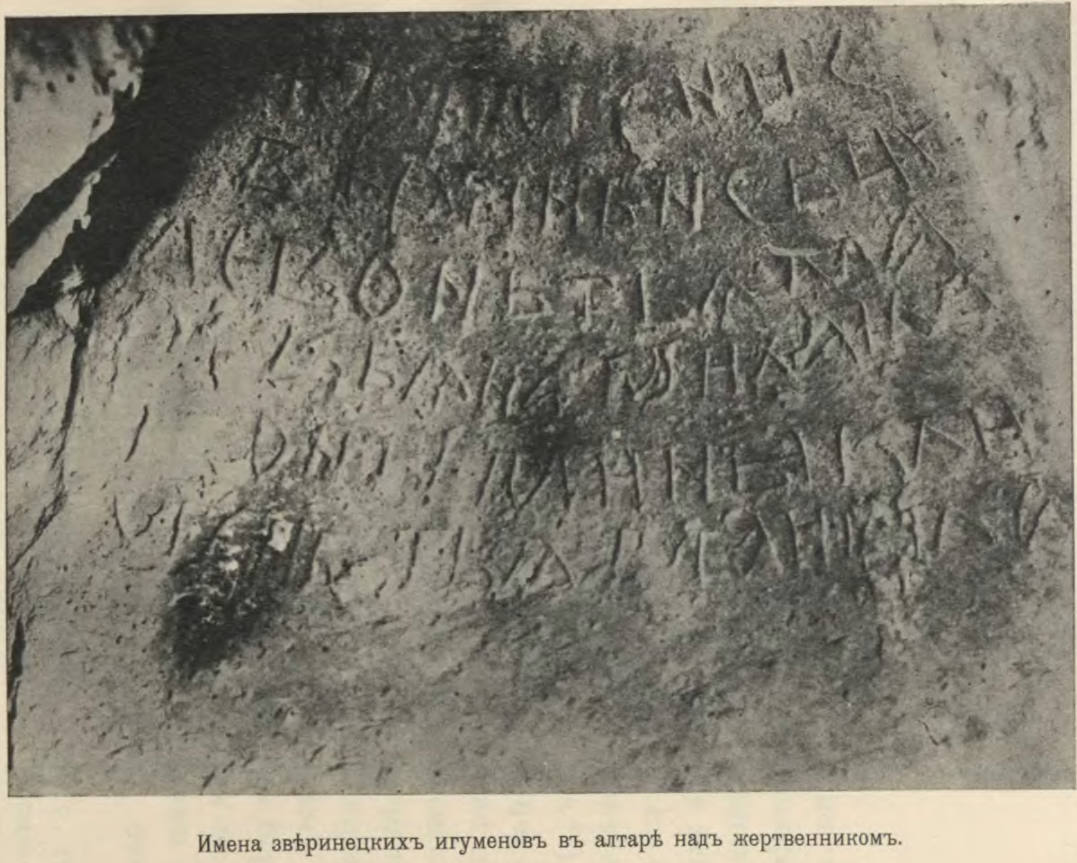
\includegraphics[width=\linewidth]{chast-colebanie-osnov/nachalo/zverp-04.jpg}
\end{center}

\vspace*{\fill}

\newpage

\begin{center}
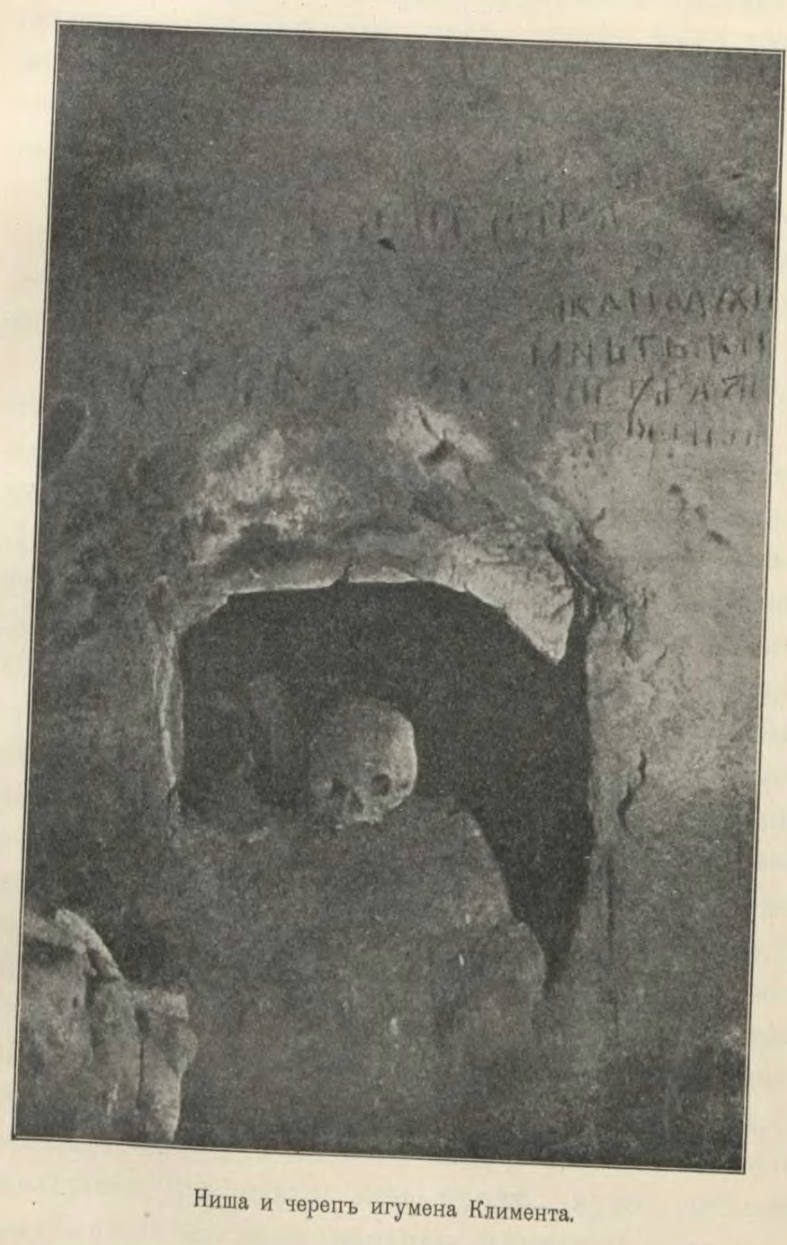
\includegraphics[width=0.95\linewidth]{chast-colebanie-osnov/nachalo/zverp-05.jpg}

\textit{Обратите внимание на соотношение глазных впадин к черепной коробке. У взрослого обычного человека черепная коробка – меньше.}
\end{center}

Что же, мы рассмотрели все надписи в пещерах. Негусто, ежели пещера использовалась людьми по крайней мере в 10, 11 и 17 веках, и если допустить, что пещера 30 лет посещалась досужими людьми, а также была наводнена зеваками в 1882 и 1888 годах.

Николай Петров задался вопросом – а так ли стары надписи на стенах?

\begin{quotation}
Некоторые из этих надписей появились, так сказать, на наших глазах, и появлялись они как бы по мере надобности в них. [...]

Далее, все подписи в новооткрытых Зверинецких пещерах начертаны одинаково, как бы рукой одного человека, – как признают это и Эртель, и г. Каманин.
\end{quotation}

Я опускаю доводы Петрова в пользу подделки надписей – желающие прочтут сами в его книжке. Не могу судить, насколько они справедливы, их нельзя однозначно ни подтвердить, ни опровергнуть. Если у нас есть выцарапанная на суглинной стене надпись, невозможно точно судить о времени ее создания, разве что по сохранности и другим надписям получится распознать, какие сделаны раньше, а какие позже.

Так что же думать? 

Все надписи были подлинно старинными, допустим 11 века? Подлинными была часть надписей, а остальные – поддельными? Все надписи, упомянутые Каманиным – подделки? Если да, то разве стены могли быть чистыми? Может, на них существовали какие-то другие граффити, а их уничтожили и написали новые, придумав для пещер историю?

А как датировать другие найденные там предметы, те же пояса?

Кожаный пояс с точно такими, как на зверинецких поясах, тиснёными иконками и надписями был в саркофаге княгини Евдокии Донской (вдовы Дмитрия Донского) в основанном ею Вознесенском монастыре московского Кремля. Княгиня была похоронена в 1407 году, но ведь могла носить пояс, уже в то время считавшийся древним.

Вот часть этого пояса – посередине изображены сцены Воскресения и Вознесения, с подписями (тоже в рамках) слева от каждой иконки:

\begin{center}
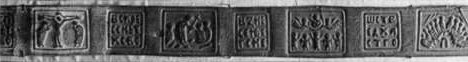
\includegraphics[width=\linewidth]{chast-colebanie-osnov/nachalo/tis02.jpg}
\end{center}

А вот часть зверинецкого – те же самые сцены:

\begin{center}
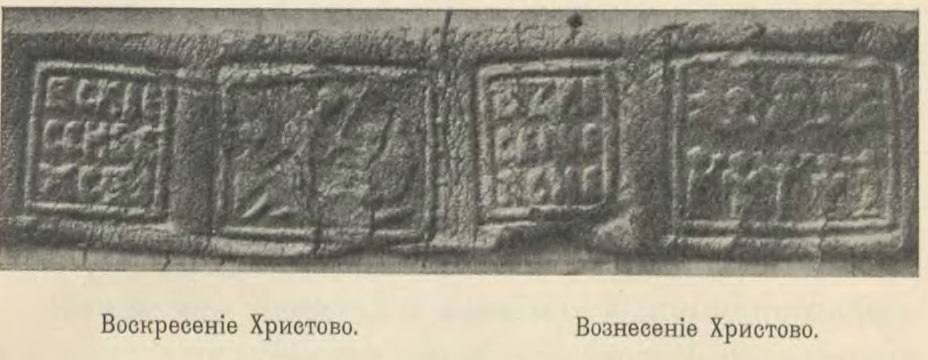
\includegraphics[width=\linewidth]{chast-colebanie-osnov/nachalo/tis01.jpg}
\end{center}

Такие же иконки (я говорю о точном подобии) тиснились на параманды – прямоугольные кожаные штуковины, носимые монахами на груди. Параманд с иконками как на «зверинецких» поясах был найден в княжеском саркофаге захоронения 14 века в 1836 году при ремонте Спасо-Преображенского на Бору собора Московского Кремля. Там же был и кожаный пояс.

Значит, по крайней мере на рубеже 14-15 веков люди носили религиозные изделия с тиснением, выполняемым одинаковым штампом. Не знаю, в разных ли местах делали эти пояса и параманды, или в одном и потом распространяли по Руси, и с какого века по какой. Определение нижней временной границы позволило бы понять, с какого времени эти пояса могли попасть в Зверинецкие пещеры.

\begin{center}
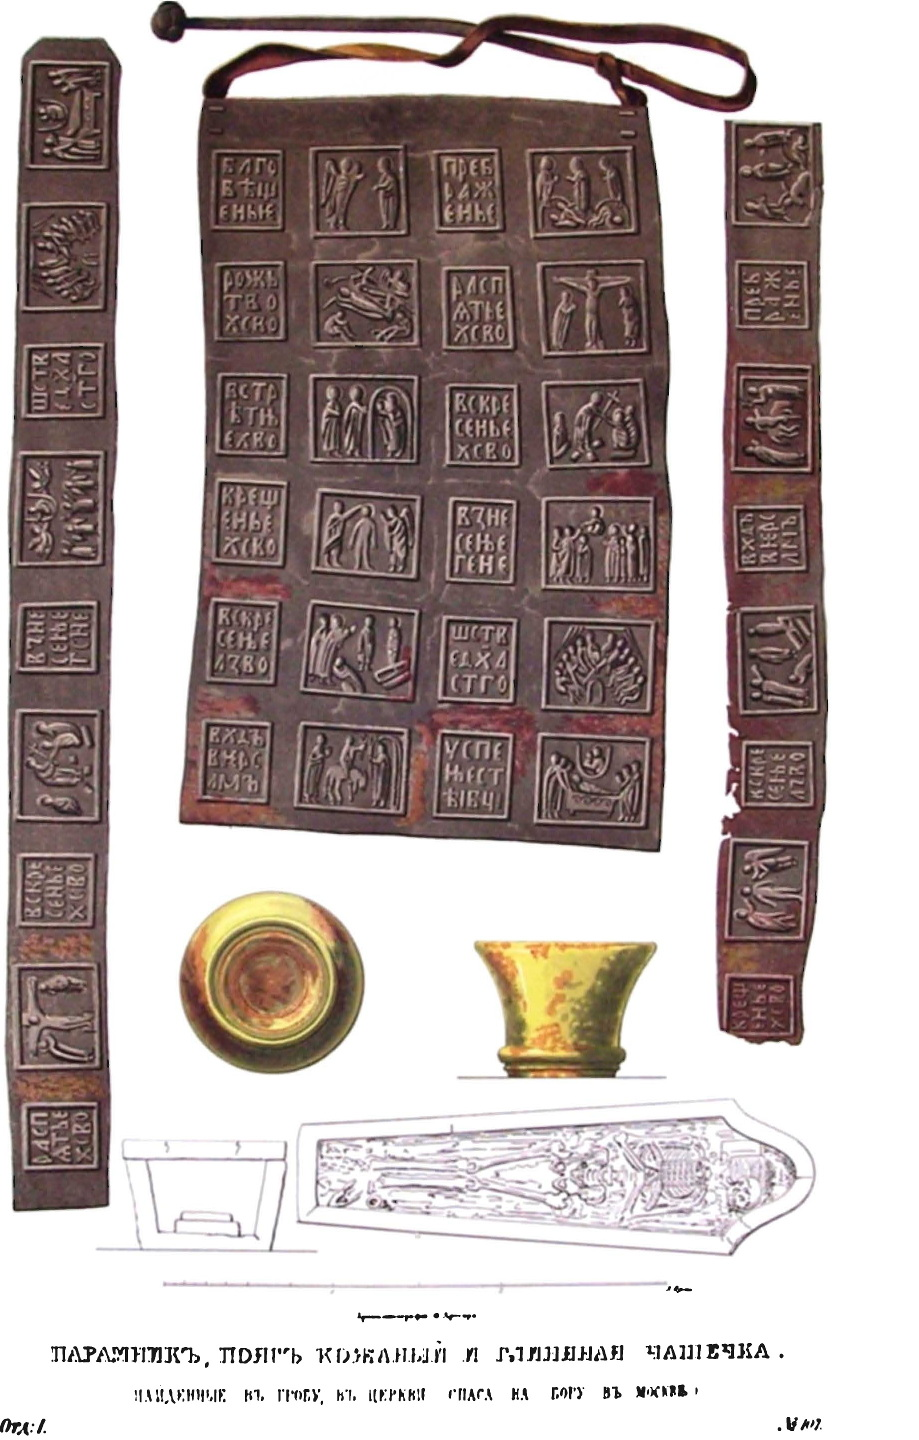
\includegraphics[width=0.94\linewidth]{chast-colebanie-osnov/nachalo/s-Drevnosti_RG_v1_ill108.jpg}
\end{center}

\textit{Из Спасо-Преображенского собора на Бору. Рисунок Фёдора Григорьевича Солнцева из книги «Древности Российскаго государства», отделение II, 1851 год.}

\newpage

%zver-pred.jpg

%Достаточно хорошо сохранились плетеные из кожаных ремешков кресты, и части поясов с выдавленными на них библейскими сценами. 

А на груди «игумена звериньского» Климентия, а точнее тела, лежащего в его поименованной нише, нашли кипарисовую (по словам Каманина) панагию – образ Богоматери с изображениями на обеих сторонах. Но панагию носили архимандриты, не игумены. Сана архимандрита вроде не было во время, к которому относят Зверинецкие пещеры.

Каманин, разбирая надпись на панагии, пришел к выводу, будто принадлежала она «Михаилу-сирину», первому киевскому митрополиту Михаилу, который, по Никоновой летописи и Степенной книге, пришел вместе с Владимиром крестить Русь и коему многие историки отказывают в существовании – мол, не было такого митрополита. Каманин же считал, что Михаил похоронен именно в Зверинецких пещерах, вероятно в «первых», открытых в 1882 году.

Николай Петров осматривал панагию и пришел к выводу, что она вовсе не кипарисовая, а оттиснута штемпелем на куске распаренного воловьего рога, и прочитал на ней первые две строчки стиха, составленного, по словам профессора, не ранее 17 века и написанные гражданским шрифтом не ранее 18 века. «Ни о каком митрополите Михаиле Сирине не может быть и речи», – заключил Петров.
\vspace*{\fill}
\begin{center}
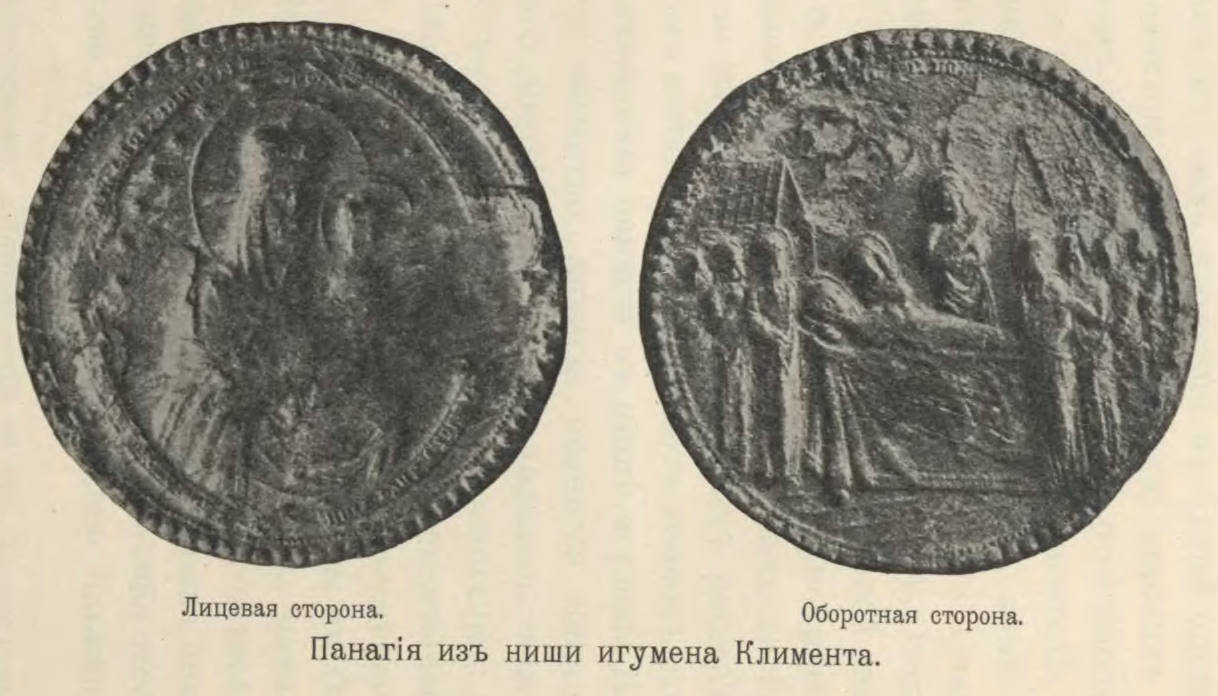
\includegraphics[width=\linewidth]{chast-colebanie-osnov/nachalo/panagia.jpg}
\end{center}
\vspace*{\fill}
\newpage

\begin{center}
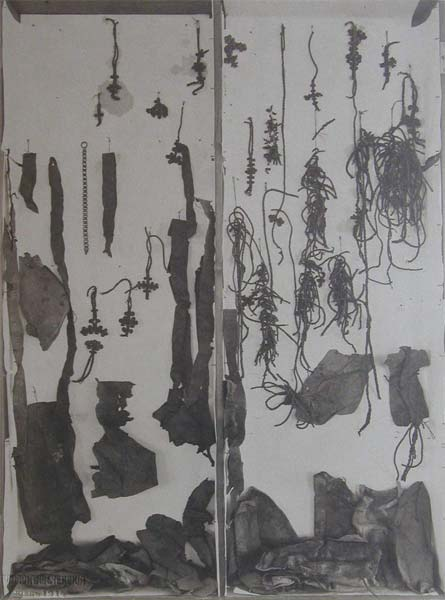
\includegraphics[width=\linewidth]{chast-colebanie-osnov/nachalo/zver-pred.jpg}
\end{center}

\textit{1914 год. Выставленные для паломников, как находки из пещер, предметы старины.}

Сомневался Петров и в древности главной находки, иконы, которую обнаружили в нише Климентия. Икона овальная, на толстой железной пластинке, покрытой эмалью, поверх которой уже писалось красками.

%У Каманина в книге, на фотографии икона выглядит иначе. 

Со времен тех дореволюционных считается, что это Одигитрия («Путеводительница») – изображение Богородицы с младенцем Христом на левой руке. Вот только нарисованное здесь далеко отлично от большинства подобных икон. Нет присущей Одигитрии сокращенной подписи «Митир Фэу Иисус Христос» («Матерь Божья Иисус Христос»). Нет нимбов. Реалистичная манера в изображении фигуры и одежды маленького. И у него странное лицо! Течение времени, повреждения краски? Да не так уж она и повреждена. Вот дореволюционный снимок:

\begin{center}
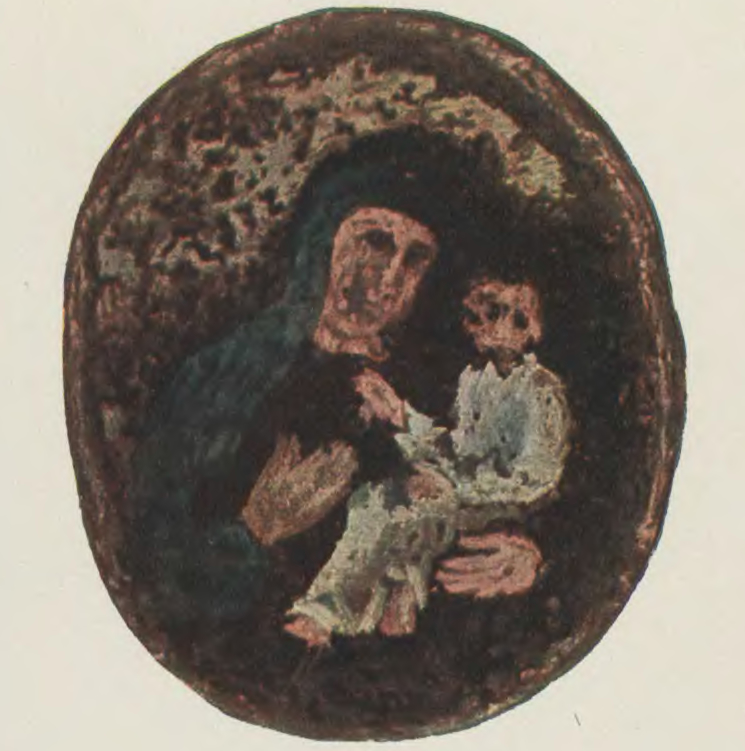
\includegraphics[width=\linewidth]{chast-colebanie-osnov/nachalo/zver-ikon.jpg}
\end{center}

Не послужит ли загадочная икона ключом к разгадке тайны Зверинецких пещер? А ведь эта икона была, коли прав Каманин, одной из древнейших славянских икон, дошедших до 20 века. Если не самой древней. 

%Нет на ней и присущей Одигитрии надписи вида: 

%\begin{center}
%\includegraphics{osn-kiev/odigitria-nadpis.png}
%\end{center}

В 1934 году, когда скит над пещерами (имевший адрес Ломаковская, 12) закрыли, икона исчезла. В разных источниках можно прочитать, что эта же икона была «чудесно обретена» в 2000-м году. Однако нашли, в 1999 году, в церкви села Селище Барышевского района, только серебряный оклад от иконы, подаренный в свое время Жеваховым.

А новую икону нарисовал в 2000 году художник А. Вовченко по дореволюционному снимку, причем с отличиями от него. Эту-то современную икону в окладе начала 20 века показывают теперь в Святотроицкой церкви Ионинского монастыря.
  
\begin{center}
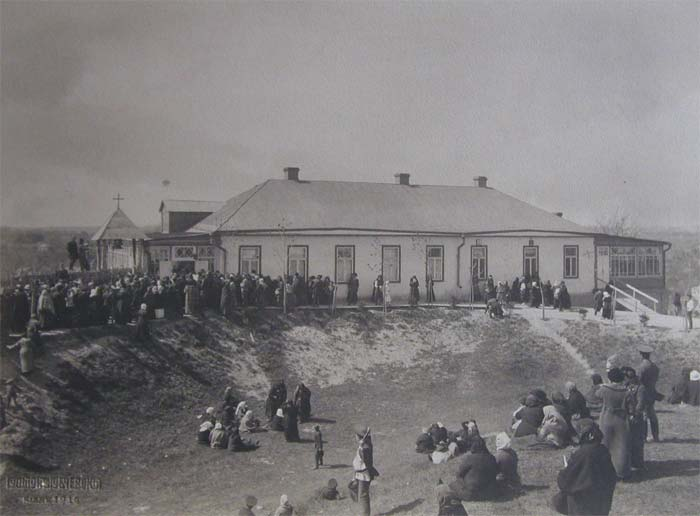
\includegraphics[width=\linewidth]{chast-colebanie-osnov/nachalo/1914-kresthod.jpg}

\textit{Окрестности Зверинецких пещер в 1914 году во время крестного хода сюда из Лавры. Возможно, фотограф стоит спиной к склону с пещерой, лицом к улице Ломаковской (Мичурина).}
\end{center}

%Пишу «Климента», а ведь надобно принять во внимание, что мы судим по найденным в пещерах надписях – а время их обнародования совпадает с раскопками Эртеля. Там был список игуменов, некоторые другие надписи, в частности две около ниши, которую сопоставили с Климентом. Надписи, по мнению Эртеля и Каманина, были древними, эдак 11 века – собственно Каманин в книге своей пытается навести мосты между летописями и списком зверинских игуменов. 

%Подвергая сомнению давность панагии и образа Богородицы, 

После открытия Зверинецких пещер 1911 года, около них создали подчиненный Лавре скит на 40 монахов и возвели церковь во имя Рождества Пресвятой Богородицы с боковым пределом, посвященным св. Иоасафу, чудотворцу Белгородскому – тому самому родичу князя Жевахова.

Предводительствовал отец Валентин (Коротенко), перешедший сюда игумен Ионинского монастыря. Валентин одолжил у Жевахова подъемные деньги, 1700 рублей и стал принимать вклады от желавших поселиться при строящейся обители. Доход приносили и паломники.

Деятельность братии и богомольцев привела к тому, что пещеры начали осыпаться. В 1913 году раскопки приостановили. Между тем продолжали впускать паломников. 

\begin{center}
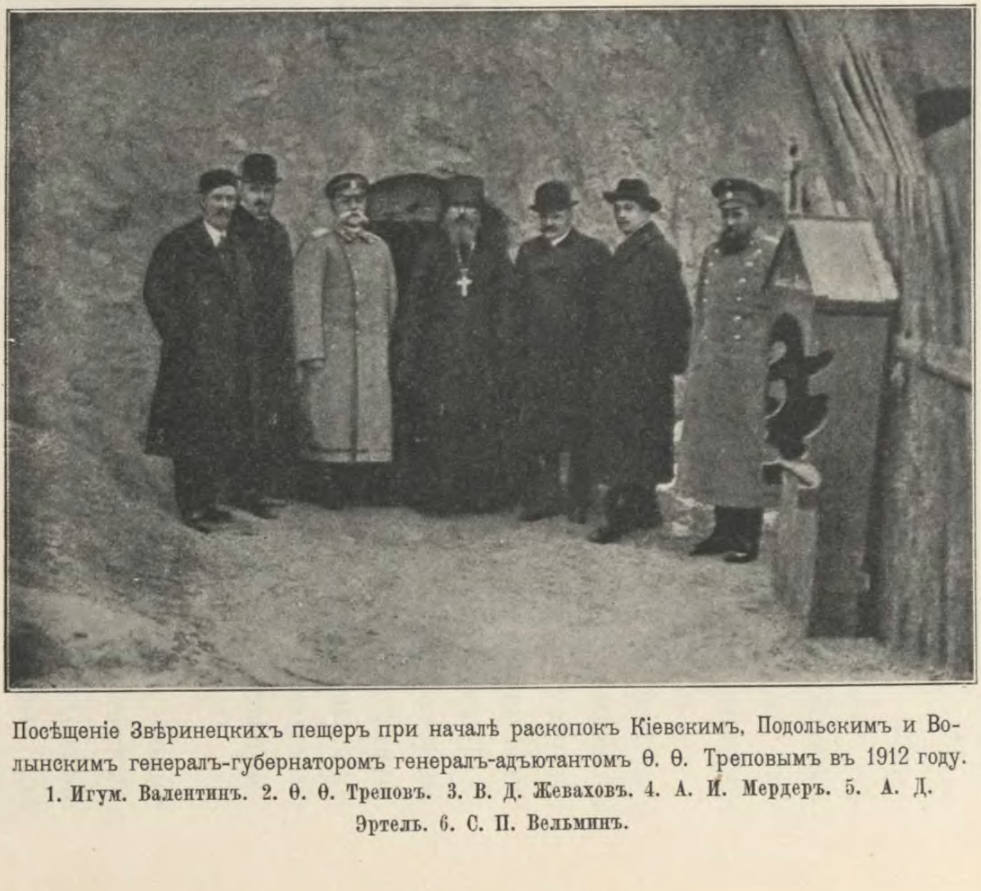
\includegraphics[width=\linewidth]{chast-colebanie-osnov/nachalo/zverp-06.jpg}
\end{center}

В 1914 году Эртель настаивал на закрытии пещер для паломников, чтобы не усугублять. И казалось бы настоял, да вышло иначе. Валентина отстранили, что, впрочем, не могло вернуть пещеры в первоначальное состояние. 

\newpage
\vspace*{\fill}
\begin{center}
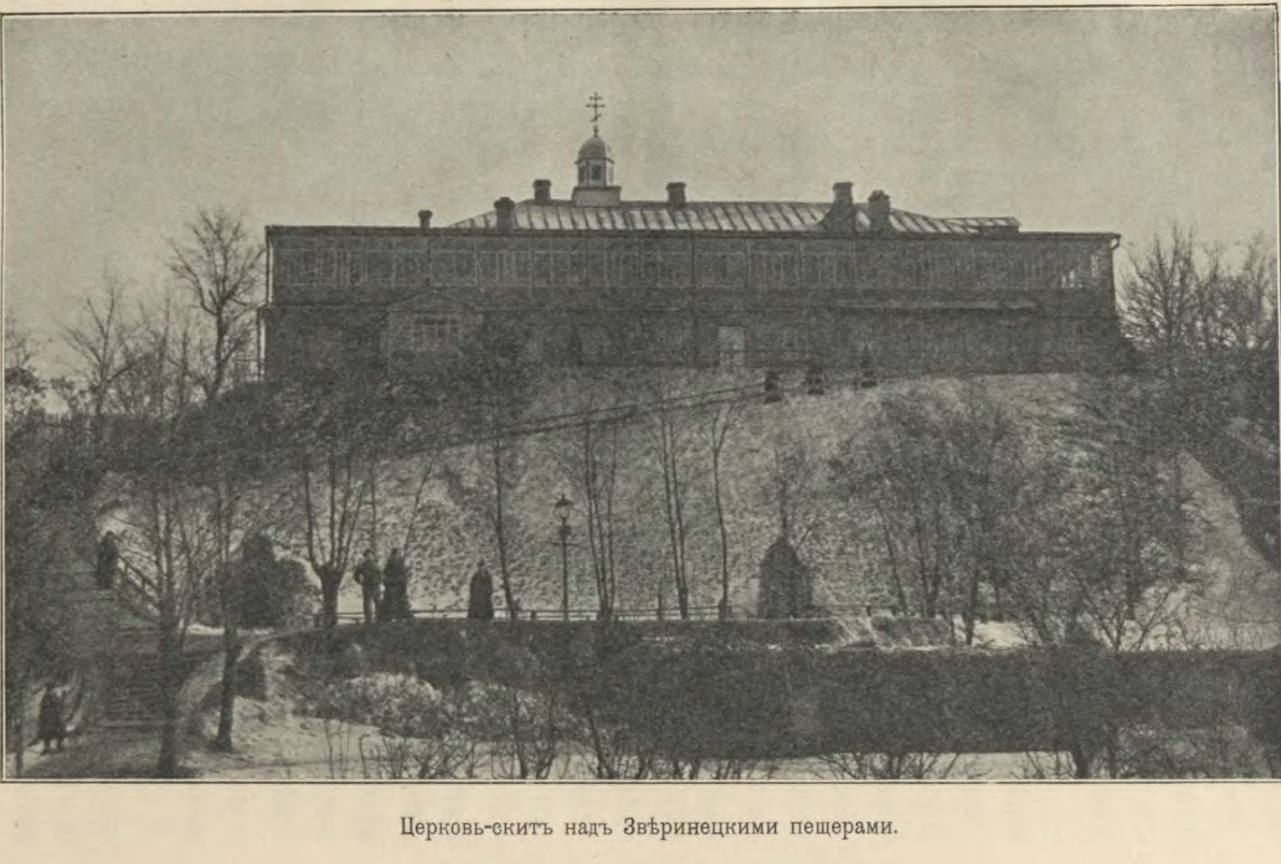
\includegraphics[width=\linewidth]{chast-colebanie-osnov/nachalo/zverp-01.jpg}
\end{center}

\begin{center}
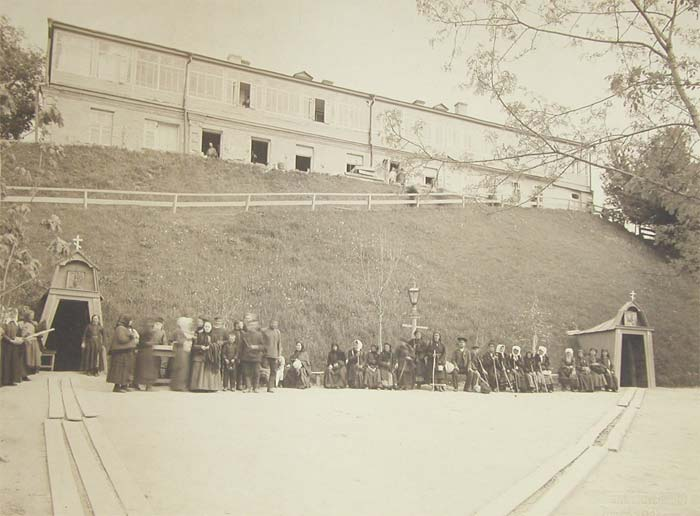
\includegraphics[width=\linewidth]{chast-colebanie-osnov/nachalo/1914-szap.jpg}

\textit{Там же, тоже вид с запада. Наверху нынче ботсад.}
\end{center}
\vspace*{\fill}
\newpage

При временном духовном безначалии – читай, при Жевахове – в 1915 году, по причине возведенного сверху подземелья храма, часть пещерных ходов укрепили оштукатуренным кирпичом, другую часть – досками. Затем скит перешел под управление иеромонаха Никанора, с которым даже Жевахов не сумел договориться о продолжении археологических работ и ремонте пещер. 

\begin{center}
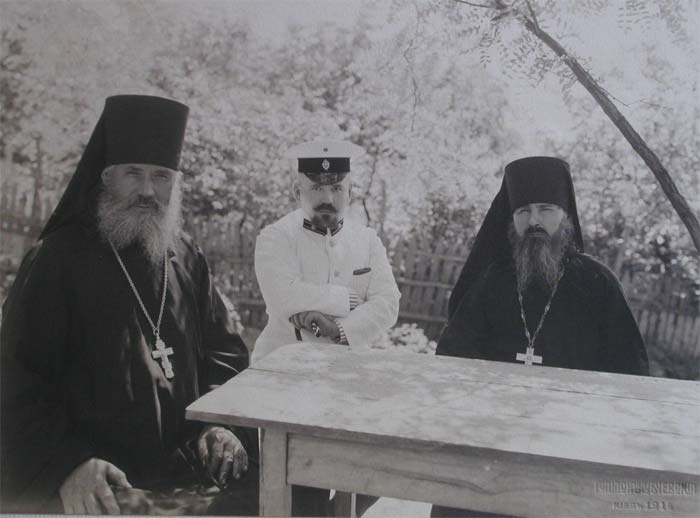
\includegraphics[width=0.90\linewidth]{chast-colebanie-osnov/nachalo/1914-nikanor.jpg}

\textit{1914. Слева направо: Никанор, Жевахов, Валентин.}
\end{center}

Разве что в 1917 году, когда очередной участок пещер стал совсем уж аварийным, Никанор разрешил позаботиться о подземельи, но с пользой для скита, дабы впридачу починили крышу надпещерной церкви. В том же году в Зверинецких пещерах похоронили отца Валентина.

Еще один удар по пещерам нанес в 1918-м\footnote{В 1918 году скит вышел из ведомства Лавры и перешел к монастырю в Церковщине (куда в марте, опасаясь большевиков, с братом Николаем скрылся Владимир Жевахов, к августу того же года впрочем ставший чиновником по особым поручениям при Министерстве внутренних дел правительства гетмана Скоропадского), а в 1925-м обрел самостоятельность.} взрыв летом пороховых складов Зверинецкой крепости, обваливший часть коридоров. Скит на поверхности тоже потерпел разрушения. Несколько позже взамен прежней церкви построили новую, в честь иконы Богоматери «Всех скорбящих радость». В окрестностях при взрыве открылись еще два пещерных хода.

В то время Киев был под немцами и гетмане Скоропадском. Его правительство сразу после взрыва объявило, что построит на разрушенном Зверинце свой центр, состоящий из Сейма, Сената, Генштаба, зданий 12 министерств.

Осенью 1918 года известному спелеологу и археологу, кстати выпускнику Киевской Духовной Академии, Игнатию Яковлевичу Стеллецкому\footnote{Большую книгу Стеллецкого «Подземный СССР» так и не издали. Впрочем опубликованы другие его работы о подземельях, среди них книга, посвященная поискам библиотеки Ивана Грозного.} поручили провести исследование подземных пустот Зверинца – выдержат ли навалившуюся власть? Стеллецкий подбирался к здешним пещерам еще в 1913 году, но Эртель не захотел тогда сотрудничать. И вот в январе 1919 года Стеллецкий приступил к работе. В марте привлек к раскопке и Эртеля, которого год назад завалило под землей на Ломаковской, с повреждением таза, руки и переломом ноги. Кажется, Стеллецкого больше заботила не застройка Зверинца, а сами пещеры. Он писал:

\begin{quotation}
В археологическом отношении встала передо мной тяжелая, значительная и в полной мере интересная задача – доказать, что открытые уже пещеры на Зверинце есть только продолжение катакомб старинного пещерного Выдубицкого монастыря непосредственно соединенного подземными нитками – соединениями с современным наземным Выдубицким в такой же мере, как так называемые Ближние или Дальние пещеры с Печерской Лаврой.
\end{quotation}

Также, Стеллецкий считал, что все эти пещеры были вырыты еще в неолит, а монахи лишь приспособили их под свои нужды.

Дневники раскопок и статьи Стеллецкого хранятся в Российском государственном архиве литературы и искусства, 208 листов, посмотреть их у меня нет возможности. Сведения о них черпаю только из сторонних, зачастую отрывочных источников.

%Стеллецкий взялся исследовать один из возникших после взрыва провалов, что вёл в древнюю пещеру с шаровидной комнаткой, где было «детское погребение» и лежали плиты сланца, древние плоские кирпичи – плинфы, еще какие-то предметы будто великокняжеских времен. Наверх от комнатки, в сторону Зверинецких пещер шел коридор с боковыми нишами, в коих тоже были захоронения. Получается, этот провал был ниже по склону, чем Зверинецкие пещеры 1911 года.

%Другой провал, около Экономических ворот Троицкого монастыря\footnote{Я не знаю, где они находились. Экономические ворота в монастыре обычно ведут к экономическому двору, и приспособлены для проезда через них с возами. О прошлом монастыря приходится судить лишь по фотографиям, ибо документация его сгорела при памятном взрыве Зверинецкой крепости.}, явил подземелье со стенами, обшитыми истлевшими досками. Его расчистили на 21 метр. Вход туда был размыт водой. Назначение сего помещения не определили. Ни среди обычных монашеских пещер, ни крепостных подземных коридоров – потерн, с таким не сталкивались.

Вот в заметке «К истории раскопок пещер
на Зверинце в Киеве (по поводу застройки Зверинца)» Стеллецкий писал (примечания по ходу мои):

\begin{quotation}
А раз так, то окончательно загадочным является подземелье, обнаруженное котлованом возле
Экономических ворот Троицкого монастыря\footnote{Я не знаю, где они находились. Экономические ворота в монастыре обычно ведут к экономическому двору, и приспособлены для проезда через них с возами. О прошлом монастыря приходится судить лишь по фотографиям, ибо документация его сгорела при памятном взрыве Зверинецкой крепости.}.
Раскопки его дают пока такую картину.

Провал образовался в своде какого-то высокого\footnote{Какова же высота?} подземного помещения, может быть, имевшего здесь входной люк. На глубине 12–13 арш\footnote{8,53-9,26 м.}.
обозначился широкий, до 3 арш.\footnote{2,1 м.}, коридор, направлением к югу, суживающийся к полу, подобно зверинецкой пещерной церкви и расширяющийся в боках. 

Самый коридор постепенно суживается вперед и опускается вглубь. Затянут он плотно илом от стремительно затекавшей сюда воды, срывавшей разной величины доски\footnote{Обшитый досками подземный ход Стеллецкий раскапывал и за 5-й гимназией, это сейчас Суворова, 1.} и бревна, которыми был обшит ход, то и дело попадающихся в разных слоях и на разной высоте намула.

Собственно над полом нанос не добирается
вершка на два, с целью не натаптывать, а доследовать пол особо. Свод коробовый, обработан небрежно и грубо.

Может быть, в дальнейшем ход примет нормальную ширину, но пока в этом отношении он выходит из рамок всего, что мне до сих пор приходилось встречать.

А. Д. Эртель склоняется к мысли, что это -
«паттерна» – стратегический ход. Я лично этого не думаю, так как считаю, что он для этого без нужды глубокий.

Я наблюдал в Пернове кавалерийский подземный ход: он, высокий, обложенный камнем, шел сквозь вал и, не выходя из последнего, поворачивал под прямым углом вправо, шел несколько вдоль вала и затем выходил в овраг с противоположной стороны.

Образчик стратегического пехотного хода
представляет выложенный местным камнем ход вокруг крепостной стены в Пскове. Внутри этого хода характерны слухи – углубления в своде, через которые слышен наружный разговор. Само собою разумеется, что и самый ход для этого был заложен не глубоко от поверхности, всего на 1 сажень. Типичные же образчики собственно «паттерн» имеем в укреплениях на Лысой Горе, где «паттерны» проходят в валах, почти не углубляясь в материк.

Зверинецкий новооткрытый ход как нельзя
более далек от этих образчиков стратегических ходов. Он есть какая-то новая разновидность в категории таинственных подземных памятников и потому вдвойне интересным представляется его дальнейшее исследование.

Другой котлован, на противоположном конце
«Укрепления»\footnote{Как понимаю, речь идет о Зверинецкой крепости и той ее части, что от современного Розария протянулась к перекрестку, где спуск в Сиреневую аллею и дорога к Ионинской церкви. Возможно, где-то в окрестностях этой точки – 50°25'02.6"N 30°33'41.2"E.}, близ разрушенной церкви скита, на глубине около 13–14 арш. дал погребение младенца с инвентарем X–XII вв.\footnote{В другом источнике упомянута – пещера с шаровидной комнаткой, где было «детское погребение» и лежали плиты сланца, древние плоские кирпичи – плинфы, еще какие-то предметы будто великокняжеских времен.}, а вслед затем, в с.с. углу стены найдены были признаки обрушившейся пустоты, другими словами, опадающий глыбами свод какого-то подземелья.

Прокопаться в это подземелье будет легче первого, потому что оно совершенно сухое и не затянуто илом; пустота должна открыться немедленно.

Открыто на днях и еще одно подземелье,
вернее, целый лабиринт, пока, однако, не исследованный – в Троицком монастыре.
В свое время оно раскапывалось любителем-иноком, но потом засыпанная часть коридора была заложена кирпичом, а вычищенная обращена под монастырский погреб\footnote{Не о пещере ли под склоном с колокольней идет речь? Так значит, там был целый лабиринт?}.

Наконец, в Выдубицком монастыре, на подворье, соединяющем Выдубицкий монастырь через Троицкий со Зверинецким акрополем, старик-монах, правда безуспешно, пытался показать место хода, который он наблюдал здесь лет 40 тому назад.

Эти данные еще более утверждают меня в
мысли, что Выдубицкий монастырь связан подземными артериями со Зверинецкими катакомбами. 

Киев. 1919.IV.12. Игн. Стеллецкий
\end{quotation}

Стеллецкий собирался продолжать археологические работы. Застройка Зверинца тормозилась, а потом власть переменилась и вопрос отпал. Чем завершились исследования Стеллецкого, я не осведомлен.

Скит на Зверинце продолжал существовать и паломники посещали пещеры. В 1924 году Жевахов принял в скитской церкви монашество как Иоасаф, два года жил в близлежащем Ионинском монастыре, а в 1926 перебрался в Зверинецкий скит и получил сан епископа. Последующие 11 лет, с перерывами – лагерь, ссылка, тюрьма – и так до расстрельного приговора тройки при УНКВД по Курской обл. 04/12/1937 по обвинению в «руководстве контрреволюционной фашистской организацией церковников». Приговор был исполнен в тот же день.

В 1934 году скит закрыли, постройки со временем разобрали. В 1980-х я нашел на его месте дореволюционный кирпич, кажется с клеймом «Х.ВОЛКОВЪ».

В 1965-м в Зверинецких пещерах провели археологическую разведку, о которой я знаю только, что исследователи установили, будто во время фашистской оккупации в пещерах прятались люди. В том же 65-м исторический памятник получил охранный паспорт\footnote{
\begin{quotation}
Взято під охорону згідно постанови Ради Міністрів УРСР № 711 від 21.07.1965 р.

Охоронний №: 139

Межі охоронної зони і зони регулювання забудови: згідно рішення виконкому Київської міської Ради народних депутатів № 920 (додаток І, п. 1, 2, 3) Звіринецькі печери входять в зону археологічного заповідника (р-н Видубицького монастиря та Звіринецькі печери). 
\end{quotation}

В указанном постановлении 711 в разделе III «ПАМ'ЯТНИКИ АРХЕОЛОГІЇ», под номером 
139 указаны «Звіриницькі печери, Печерський район, Звіринець» – с примечанием «з настінними написами (XI-XIII ст. ст.)». Постановление было отменено 03 сентября «Постановой КМ № 928 (928-2009-п)», и тогда же пещеры занесли в новый реестр, Государственных недвижимых памятников Украины, как объект культурного наследия под номером 260034-Н – археологический памятник 11-17 веков, по адресу Мичурина 18-22.}, переоформленный в 2009 уже для нового реестра.

В 1979 году пещеры посетили археологи из Киевской лаборатории спелеологических исследований. Тогда-то, надо полагать, и передвинули будку нужника в сторону от входа в подземелье.

На сегодня определены – их приводят в книгах\footnote{Например, «Историко-градостроительные исследования Киева» под редакцией В. Вечерского, Киев, Феникс, 2012.} – границы зоны охраны культурного слоя первой категории вокруг памятника «Зверинецкие пещеры»:

%На сегодня определены границы зоны охраны культурного слоя первой категории вокруг памятника «Зверинецкие пещеры»:

\begin{quotation}
от пересечения ул. Мичурина и переулка Мичурина по правой стороне улицы Мичурина в юго-восточном направлении (до усадьбы № 28), оттуда в юго-восточном, юго-западном и северо-западном направлениях (территория Центрального ботанического сада им. М. Гришко НАН Украины) до пересечения с ул. Мичурина.
\end{quotation}

Попытайтесь наложить это описание на карту, и у вас ничего не получится, поскольку от пересечения улицы Мичурина с переулком можно двигаться по правой стороне только на северо-восток, а не на юго-восток.

В конце 20 столетия паломничество в пещеры возродилось, Музей Киева провел реставрационные работы, одновременно добиваясь отселения жителей из усадеб на Мичурина с номера 18 по 24, на четной, подгорной стороне.

В начале 21 века в усадьбе с пещерами, при созданном монастыре, возвели собор, а окрестности постигла тяжелая перестройка. На месте скромных стареньких домиков, белеющих через листву садов, огороженных кривыми заборами, вдруг возникли терема за крепостными стенами, коих устрашился бы сам Батый.

Летом 2017 года мы с Дашей Кононюк посетили Зверинецкие пещеры, побывали там впервые. За толстой, обложенной камнем стеной усадьбы – церковные здания, соединенные друг с другом и покрывающие склон. Двери, лестницы. Всё построено добротно и основательно. В церковной лавке мы разговорились со служителем церкви, который познакомил нас со священником. Тот любезно проводил нас в пещеру и рассказал много полезного. Если о нераскопанном ходе в сторону Ионинской церкви мы знали, то сведения про нераскопанный же ход в направлении Выдубицкого монастыря был новостью.

Дойдя с нами до половины пещеры, священник оставил нас одних и мы продолжили осмотр. Несмотря на жару снаружи, внизу было столь холодно, что изо рта шел пар.

Пещера основательно укреплена, местами оштукатурена. Высота потолков в коридорах, кроме одного места, более чем достаточна для прохождения посетителей, еще с запасом. Освещения не было, кроме взятого с собой – священник и Даша держали в руках свечи, а я фонарик.

Пустые комнатки (я избегаю слова келья, указывающее на место жительства монаха) по обеим сторонам коридоров ничем не защищены, а вот наполненные костями закрыты черными коваными решетками. Некоторые имеют длину явно меньшую, чтобы там лежа мог поместиться взрослый человек обычного роста. Даже если это чисто погребальные ниши, то для тела детского или подросткового роста.

Среди комнаток были такие, где можно находиться сидя. В одной по бокам было два «лежака», а между ними выемка.

Современные Зверинецкие пещеры я могу назвать, скорее, пещерами созданными недавно на основе древних пещер, поскольку от седой старины в нетронутом виде не осталось ничего. Да и сама окружающая местность преобразилась.

\vspace*{\fill}

\begin{center}
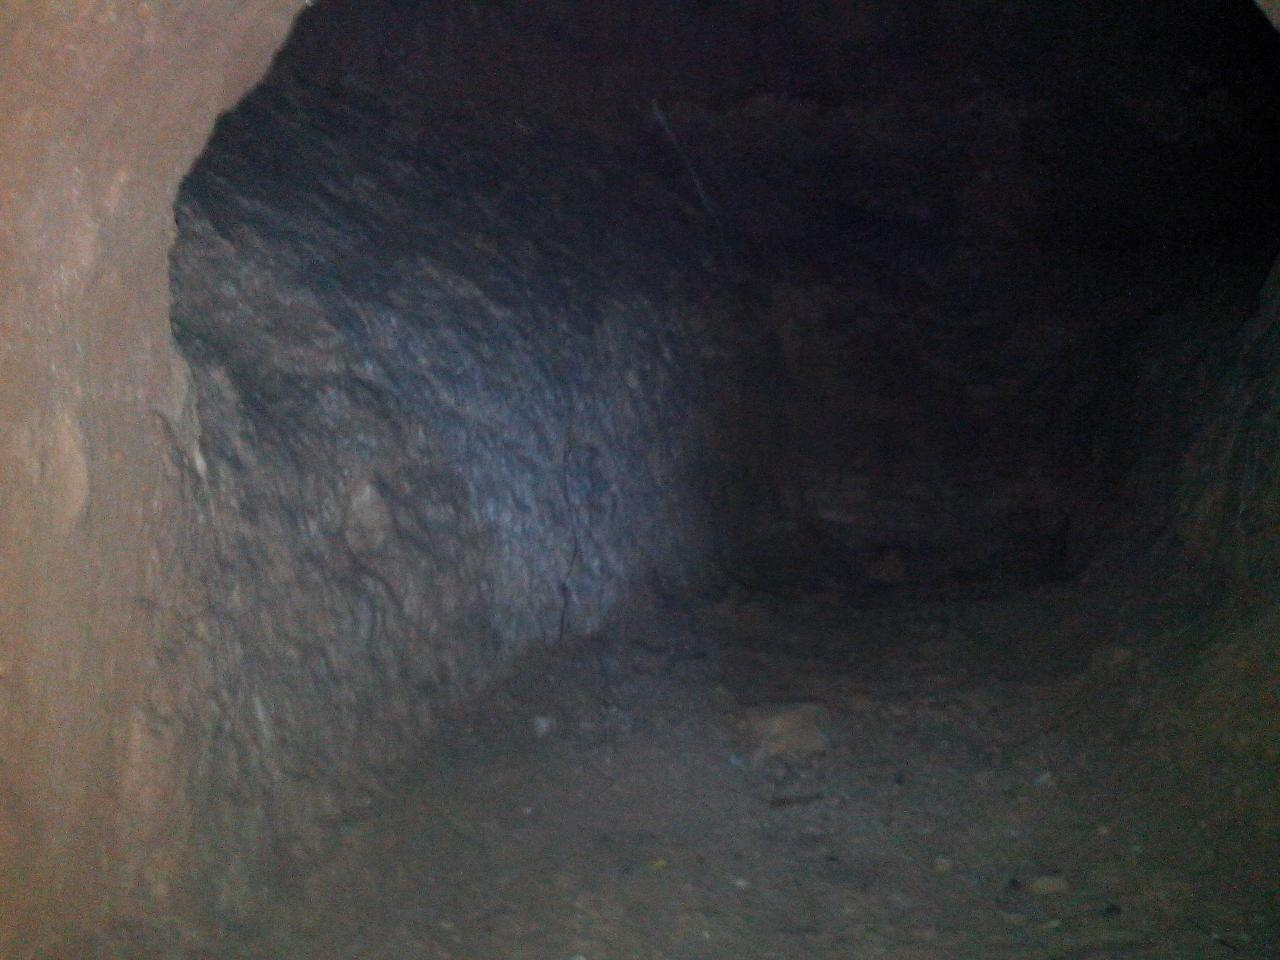
\includegraphics[width=0.98\linewidth]{chast-colebanie-osnov/nachalo/IMG_20170626_135030.jpg}

\textit{Комнатка с лежаками.}
\end{center}

\vspace*{\fill}


\newpage

\begin{center}
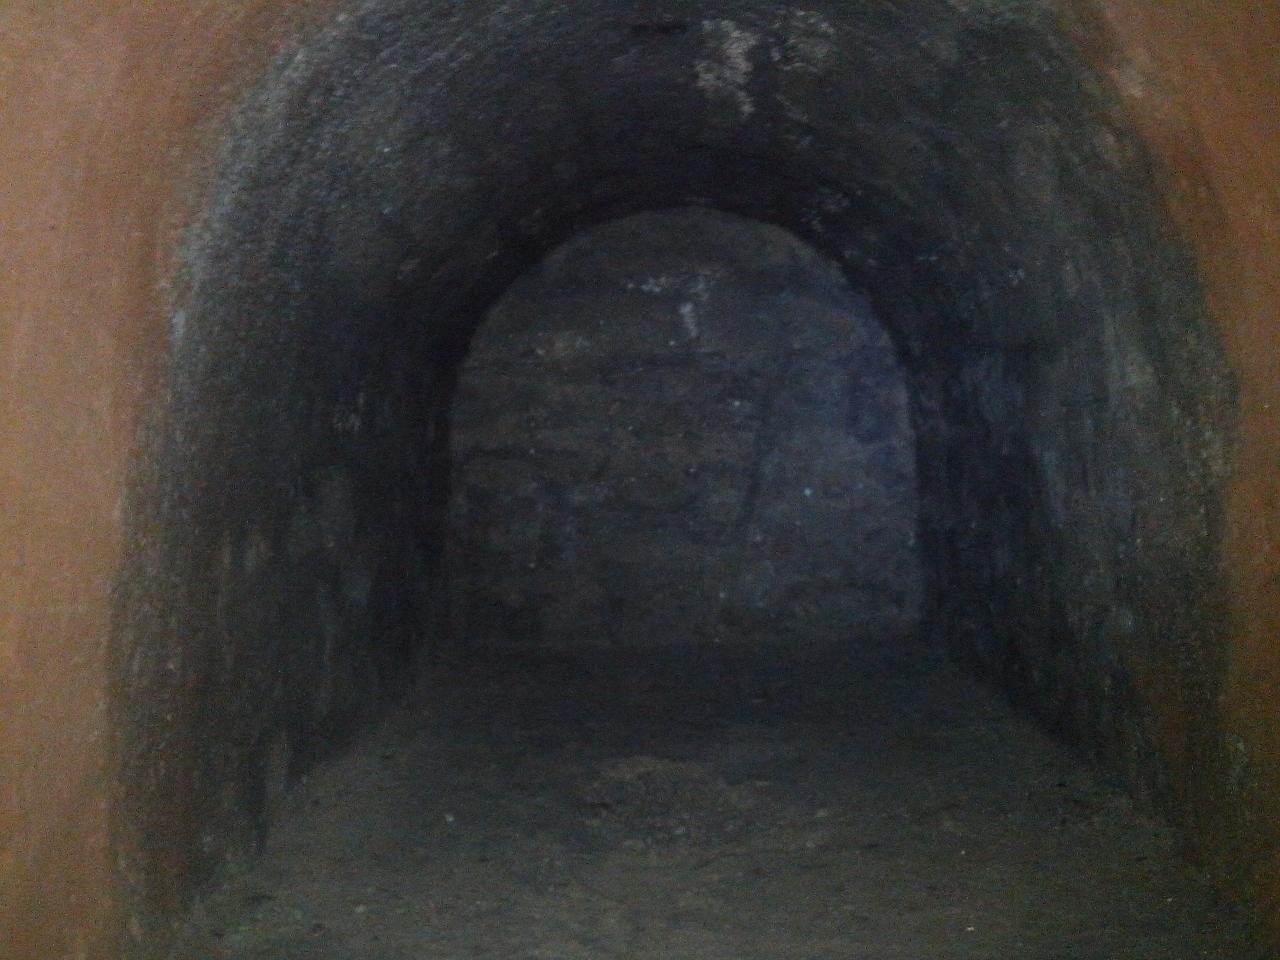
\includegraphics[width=0.98\linewidth]{chast-colebanie-osnov/nachalo/IMG_20170626_135106.jpg}

\textit{Одна из многочисленных «погребальных ниш» малой длины.}
\end{center}

\begin{center}
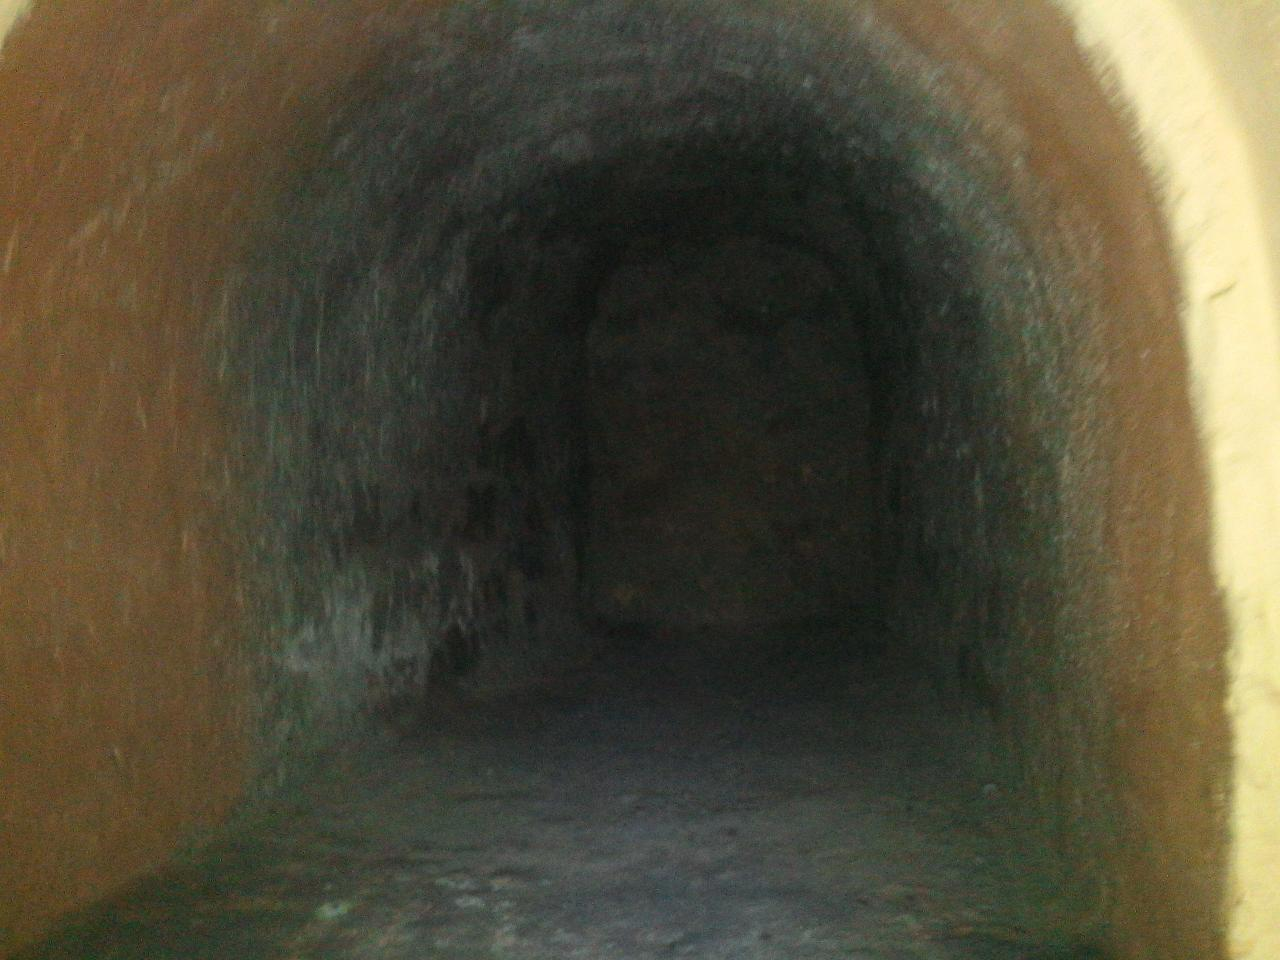
\includegraphics[width=0.96\linewidth]{chast-colebanie-osnov/nachalo/IMG_20170626_135152.jpg}

\textit{Еще одна.}
\end{center}

\newpage
\vspace*{\fill}
\begin{center}
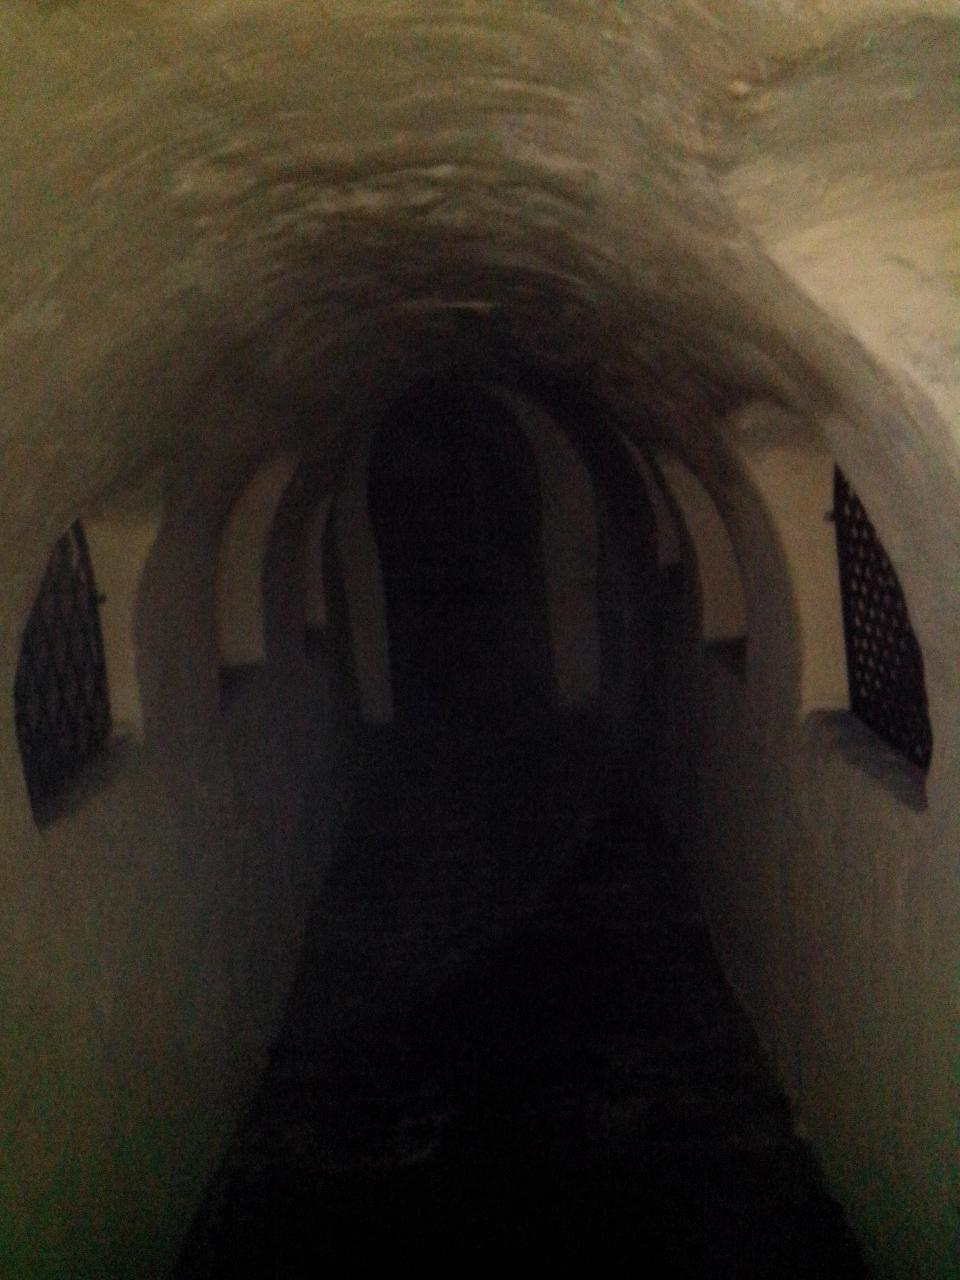
\includegraphics[width=\linewidth]{chast-colebanie-osnov/nachalo/IMG_20170626_135248.jpg}

\textit{Коридор с «погребальными нишами».}
\end{center}
\vspace*{\fill}

\newpage

\vspace*{\fill}
\begin{center}
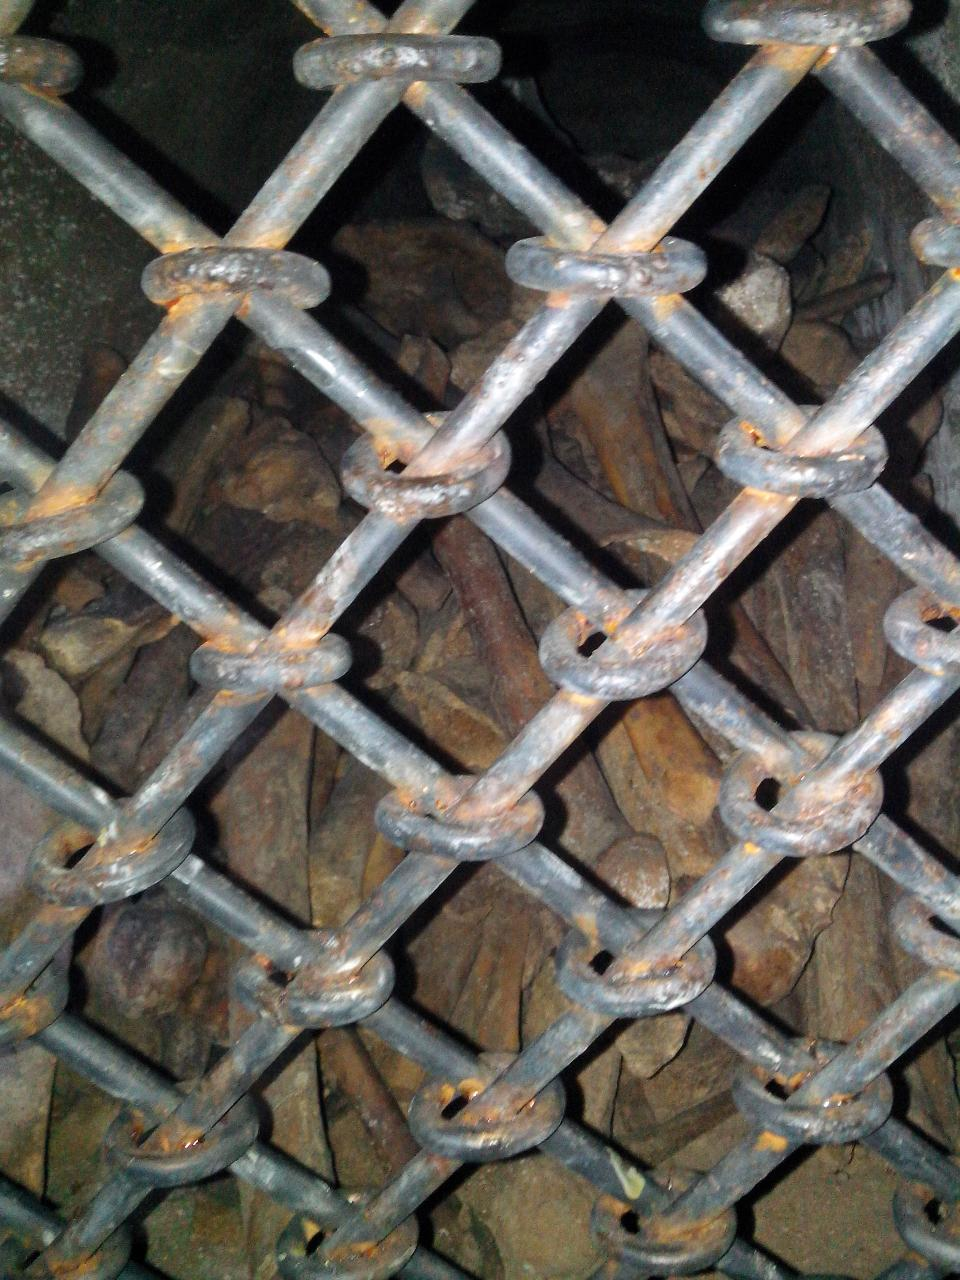
\includegraphics[width=\linewidth]{chast-colebanie-osnov/nachalo/IMG_20170626_135243.jpg}

\textit{Прах к праху. Чьи вы руки и ноги, как выглядели целыми во плоти?}
\end{center}
\vspace*{\fill}
\newpage
\vspace*{\fill}
\begin{center}
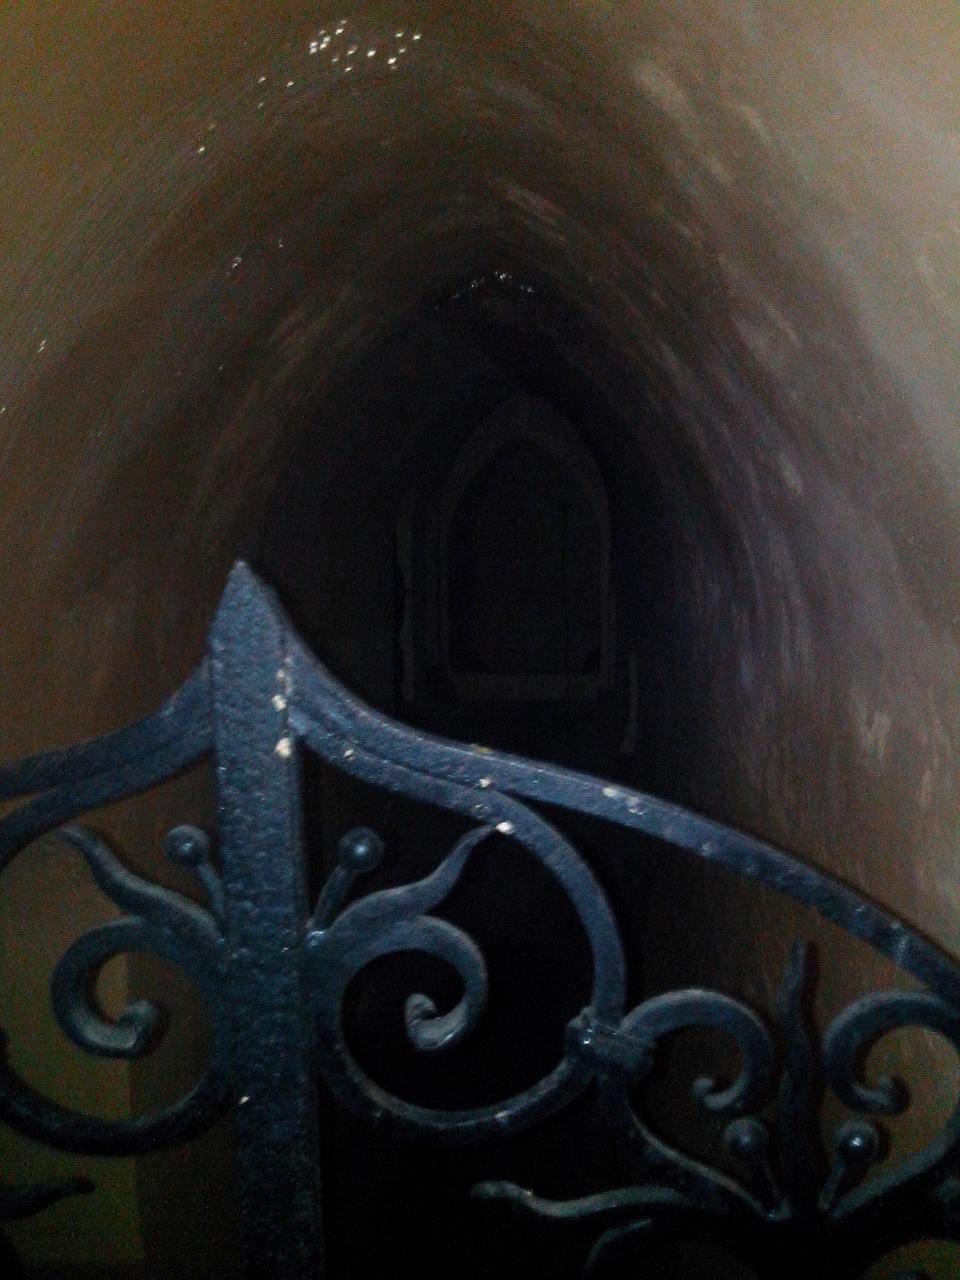
\includegraphics[width=\linewidth]{chast-colebanie-osnov/nachalo/IMG_20170626_135548.jpg}

\textit{Коридор ведет к нераскопанной части пещер. Что там дальше?}
\end{center}
\vspace*{\fill}
\newpage

Но я помню тот еще прежний, в зелени садов поворот на Мичурина, под пещерами, с домом некой бабы Даши напротив – у нее козы жили, а хатка пряталась за кустами сирени. Про пещеры я знал тогда очень смутно, мне они были до лампочки. А ведь ходил мимо почти каждый день.

Я мало увлекался этим всем, живя около ботсада и окруженный древностью со всех сторон. Не говорю об Ионинской церкви, это сравнительный новодел, а во время моего детства она была еще просто государственным зданием, там вечно происходила реставрация, я заходил внутрь, кроме строительных лесов было пусто, а вне стен, на траве валялись куски мозаики – я подобрал несколько больших кусков и хранил дома. Напротив церкви, двухэтажная старенькая колокольня с круглыми часами, на всю округу отбивала каждый час. Я слышал ее даже дома.

Ботанический сад имени Гришко расположился на буквально летописных холмах Зверинца. В глубокой ложбине спрятался монастырь Выдубичи, с его заметными куполами – на колокольне синий в звездах, а другие зеленые. На одном из окрестных склонов в седую старину был Всеволож Красный двор. Вроде бы именно его остатки нашли советские археологи в семидесятых годах на соседствующем с Выдубами, к северу, углу горы – хотя понятно, что никакой таблички с названием при раскопках не обнаружили.% Как по мне, князю выгоднее было строиться там, где в ботсаду перекресток у верха сиреневой аллеи, хвойных и дороги к Ионинской церкви.

Сейчас Красный двор, что называется, возродили – поставили на холме (в 700 метрах от Зверинецких пещер), известном как мыс Чайка,  ограду из бревен, бревенчатую же башню о двух этажах\footnote{50.421302634400284, 30.56695182662565}, и памятный камень с фамилиями тех, кто сему способствовал. В той же местности находилась гончарная слобода, эдак в столетии 13-14. Археологи нашли полные готовой посуды печи, а что случилось, почему всё бросили, неясно.

Напротив основной Зверинецкой горы, к северу – другая гора, со Зверинецким кладбищем, а за нею в удольи – Наводницкий ручей. Он бежит в коллекторе, однако до 2014 года в пойменном овраге сохранялось и поверхностное его течение, питаемое сочащимися со склона кладбища родниками. Затем на уцелевшем отрезке ручья развернули строительство и всё пропало. 

%Прежде там, на перекрестке бульвара Дружбы Народов и улицы Старонаводницкой, у подножия трех холмов – Зверинецкого, кладбищенского и с Родиной-матерью – была конечная остановка троллейбуса. 

%А еще ранее там же Неводницкий ручей, купно со стоком лежащего к юго-западу озеру Святому (о нем читайте в отдельной главе про Зверинец) образовывал озеро Проклятое, соединяющееся с Днепром. 

В восьмидесятые годы прямо рядом с кладбищем, на Верхней улице возвели больницу Четвертого управления. А вместо близлежащей высотки по третьему номеру, был частный сектор – пал жертвой строительства. Маленьким, однажды я бродил там в саду около развалин и нашел игрушки: фиолетовую уточку на колесиках, со ржавой осью, да печального резинового пёсика с пищалкой. Хорошо это запомнил, ибо тогда я впервые увидел разрушенный, снесенный дом.

Западный из южных отрогов Зверинца называется Бусовой горой, а напротив нее, через железную дорогу и летописную речку Лыбедь – Лысая, она же Девич-гора, с остатками крепости. У низовья ботсада, перед железной дорогой, возле ручья под склоном, мы с мамой опять-таки в начале восьмидесятых нашли доисторическую штуку из гладкого камня. До сих пор не знаю, что это. 

Тогда в Выдубицком монастыре помещался Институт археологии. Мы понесли штуку туда – «показать специалистам». Специалистам она оказалась пофиг, и с тех пор занимает дома почетное место на книжной полке рядом с окаменевшей ракушкой.

Смутно помню, как зашли мы в один из корпусов института, бывшее монастырское здание. Потолки высокие, стены толстые. Тихо, темновато, прохладно. Обратились к тетеньке-ученой. Она покрутила предмет в руках. Еще голову так наклоняла, сбоку набок. Потом скучно сказала, что это наверное дети баловались и вылепили из глины. Ученым такое не нужно. С тем мы и ушли.

%Уже в 2013 году я обратился за помощью с определением штуковины к археологам, в одно из сетевых сообществ. Без толку. 

Но штуковина – из кремня, а не глины. Орудия труда «каменного века» обычно лишены такой шлифовки. Поверхность нашей находки гладкая, камень удобно лежит в руке и будто, в самом деле, под нее вылеплен. А с одного конца есть ровная каёмка. Быть может, в этом месте предмет к чему-то крепился и, вращаясь (что и послужило шлифовке) был частью некоего приспособления?

%В 2013 году я наступил на грабли, попросив археологов о помощи в определении. Пошла потеха! Что же, плачевно состояние той науки, чьей представителям насмешка служит средством к познанию.

\newpage
\vspace*{\fill}
\begin{center}
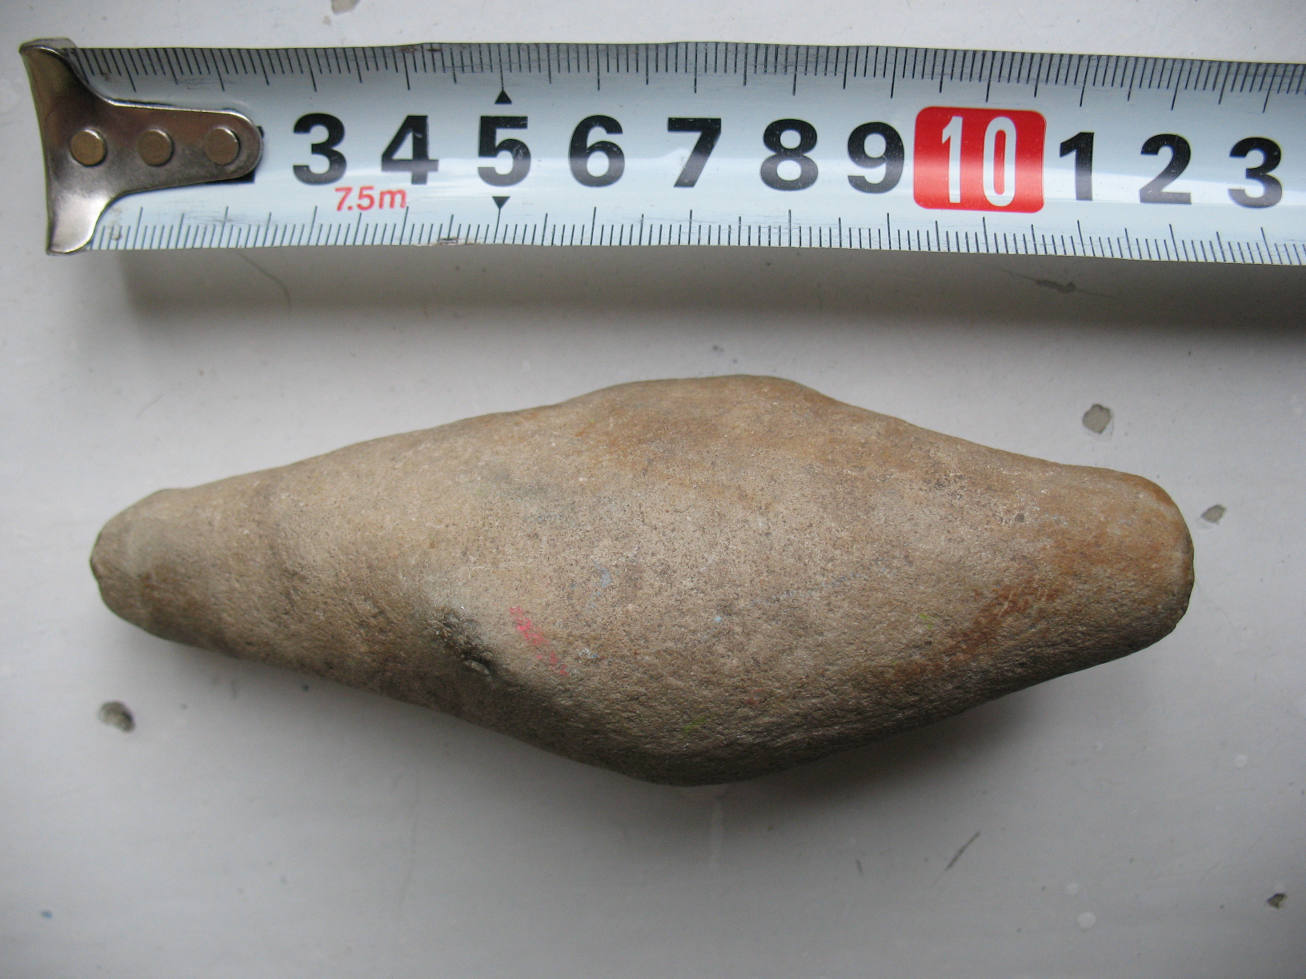
\includegraphics[width=\linewidth]{chast-colebanie-osnov/nachalo/s_figovina-01.jpg}
\end{center}

\begin{center}
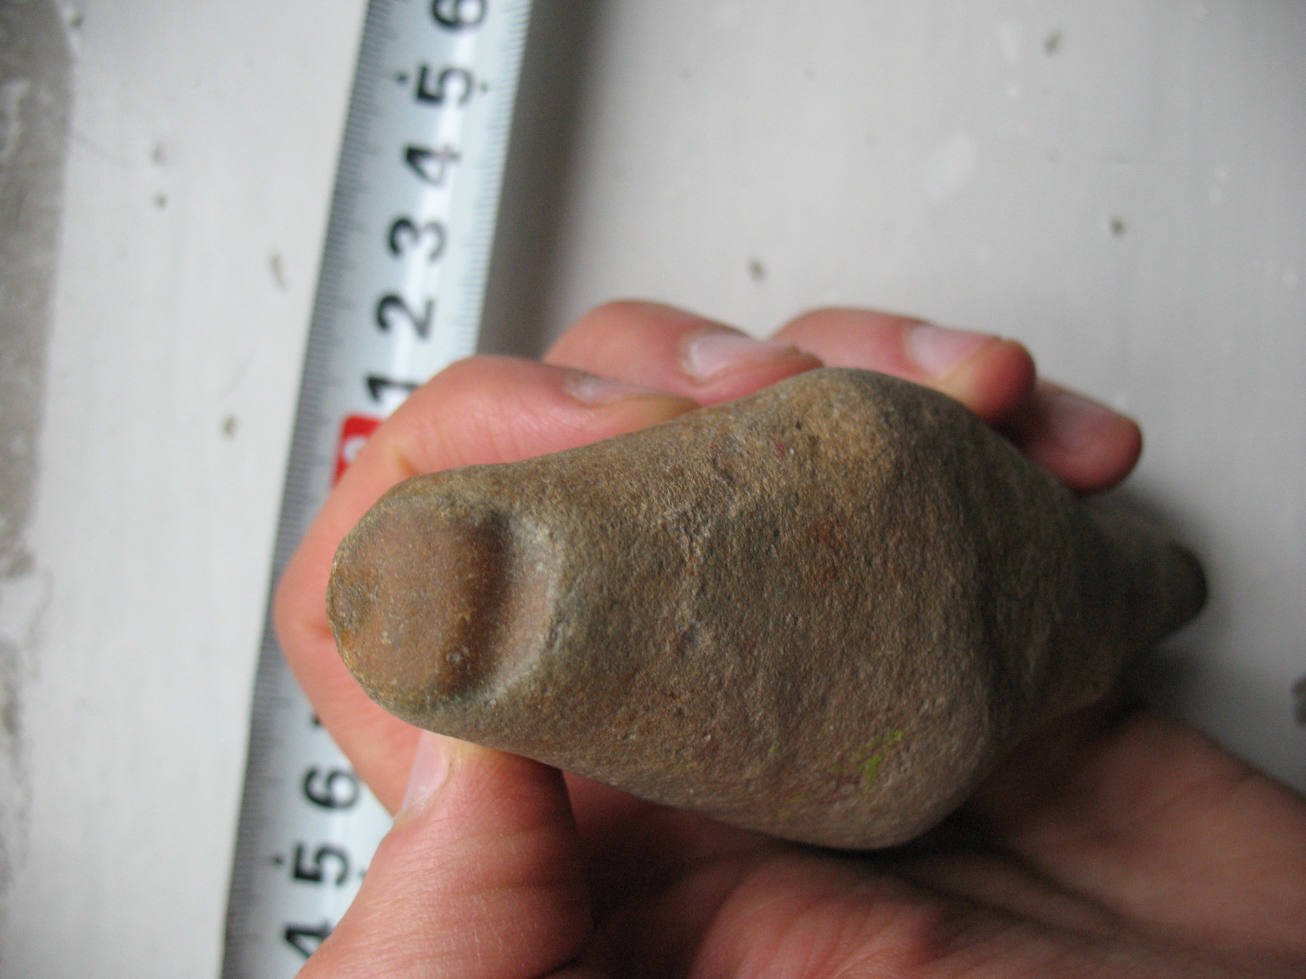
\includegraphics[width=\linewidth]{chast-colebanie-osnov/nachalo/s_figovina-02.jpg}
\end{center}
\vspace*{\fill}
\newpage

%Еще о Выдубах! В Выдубицком монастыре меня привлекала глыба базальта, черная. И глубокий колодец, могила Ушинского и прочие могилы менее именитых людей, да еще огромная ива на пригорке вне монастырских стен. Я хватался за её ветки и катался.

Расскажу подробнее, где был найден этот предмет. Мы часто гуляли «мимо ботаники», по улице Тимирязевской. С одной стороны там был бесконечный забор ботсада, увитый светло-зеленым хмелем, а с другой – захолустные усадьбы частного сектора, прорезанные сбегающими с холма проулками такими узкими, что два человека едва могли разойтись. Ниже хоздвора ботанического сада, за забором, в овраге течет ручей Омелютинка. Левый берег его, слывущий среди старожилов горой Караваевкой, высок и крут. Низовье ручья взято в коллектор. Он примерно повторяет прежний отрезок естественного русла, образовавшегося в суше после отступления вод Днепра от Зверинецкого холма.

Русло это поворачивало на север, северо-восток в сторону железнодорожной платформы Ботанической – она была на отрезке примерно между северной частью улицы Беренбойма и Деревообрабатывающей. Когда построили платформу Выдубичи, то Ботаническая загнулась и теперь о ней напоминает лишь остановка автобуса 54, и та – по требованию. Это местный маршрут, обслуживающий промзону Телички и соединяющий её с окрестностями музея Великой Отечественной войны.

На аэрофотоснимках 1943 года ручей, чуть огибая холм, впадает затем в озеро, которое было ниже Выдубицкого, отделенного от него насыпью железной дороги. Оба озера – старицы, части некогда проходившего здесь русла Днепра, рукава, что подступал под самый берег. Теперь озеро поглощено промзоной. В начале 20 века оно дотягивалось до широты конца Тимирязевской улицы, и на картах того времени обозначено как «Старик» и «Теличка», по названию местности. 

%между Зверинецкой горой и ДОКом (дерево-обрабатывающим комбинатом), и теперь поглощено промзоной. Современные границы исчезнувшего озера можно обозначить – между улицами Стройиндустрии на юге и улицей Баренбойма на севере. На одной карте Киева 1914 года озеро обозначено как «озеро Старик», на другой – как «озеро Теличка» по названии местности (деревня Теличко), причем озеро было растянуто на юг до теперешнего уровня низа улицы Тимирязевской. Стариком оно именовалось потому, что было остатками большого рукава Днепра, старым его руслом.

 %Баренбойма очень каверзная, она начинается на севере, а потом прерывается и телепортируется к метро Выдубичи!

По снимкам 1943 года видно, что от юго-восточной части озера ручей шел через пустыри и за мостом насыпи соединялся с нынешним Днепровским заливом. Сейчас ботанический отрезок ручья примечателен тем, что окрестности его кишат клещами. Некоторые участки берега, в труднодоступных местах, укреплены маленькими колышками, забота о чем прослеживается десятилетиями. Мы сняли эти укрепления в фильме «Киевская сюита», стоит посмотреть! Кто, зачем, почему?

В восьмидесятых, у самого низа улицы Тимирязевской – там сейчас сооружения тепличного хозяйства Киевзеленстроя – ручей еще не был в коллекторе, а образовывал эдакую дельту, обнятую пригорком суглинного берега. На высоте, с него гирляндами свисали засохшие ракушки нескольких видов – вроде мидий и еще каких-то длинных. Около ракушек склон казался светлым, почти белым. Встречались участки и рыжей глины – местные её копали. В небольшой пещерке невесть какого происхождения мы и нашли каменную фиговину.

Удолье у подножия холма. Островки между разветвлений ручья. Мы скакали по мягкой земле. К небу поднимались давние, громадные деревья. Из-под корней пробивался родник. Виднелись развалины частного дома, среди остатков сада росли вишни. Весной, едва пригревало солнце, появлялись цветы – фиалки, мускарики. Теплилось, веяло нерешительной свежестью. Первобытное чудесное место!

На снимке ниже, начало двухтысячных годов, может быть 2003, в дельте ручья ведется строительство. Холм частично срыт и крутизна его умерена, деревья срублены, вода загоняется в коллектор.

\vspace*{\fill}

\begin{center}
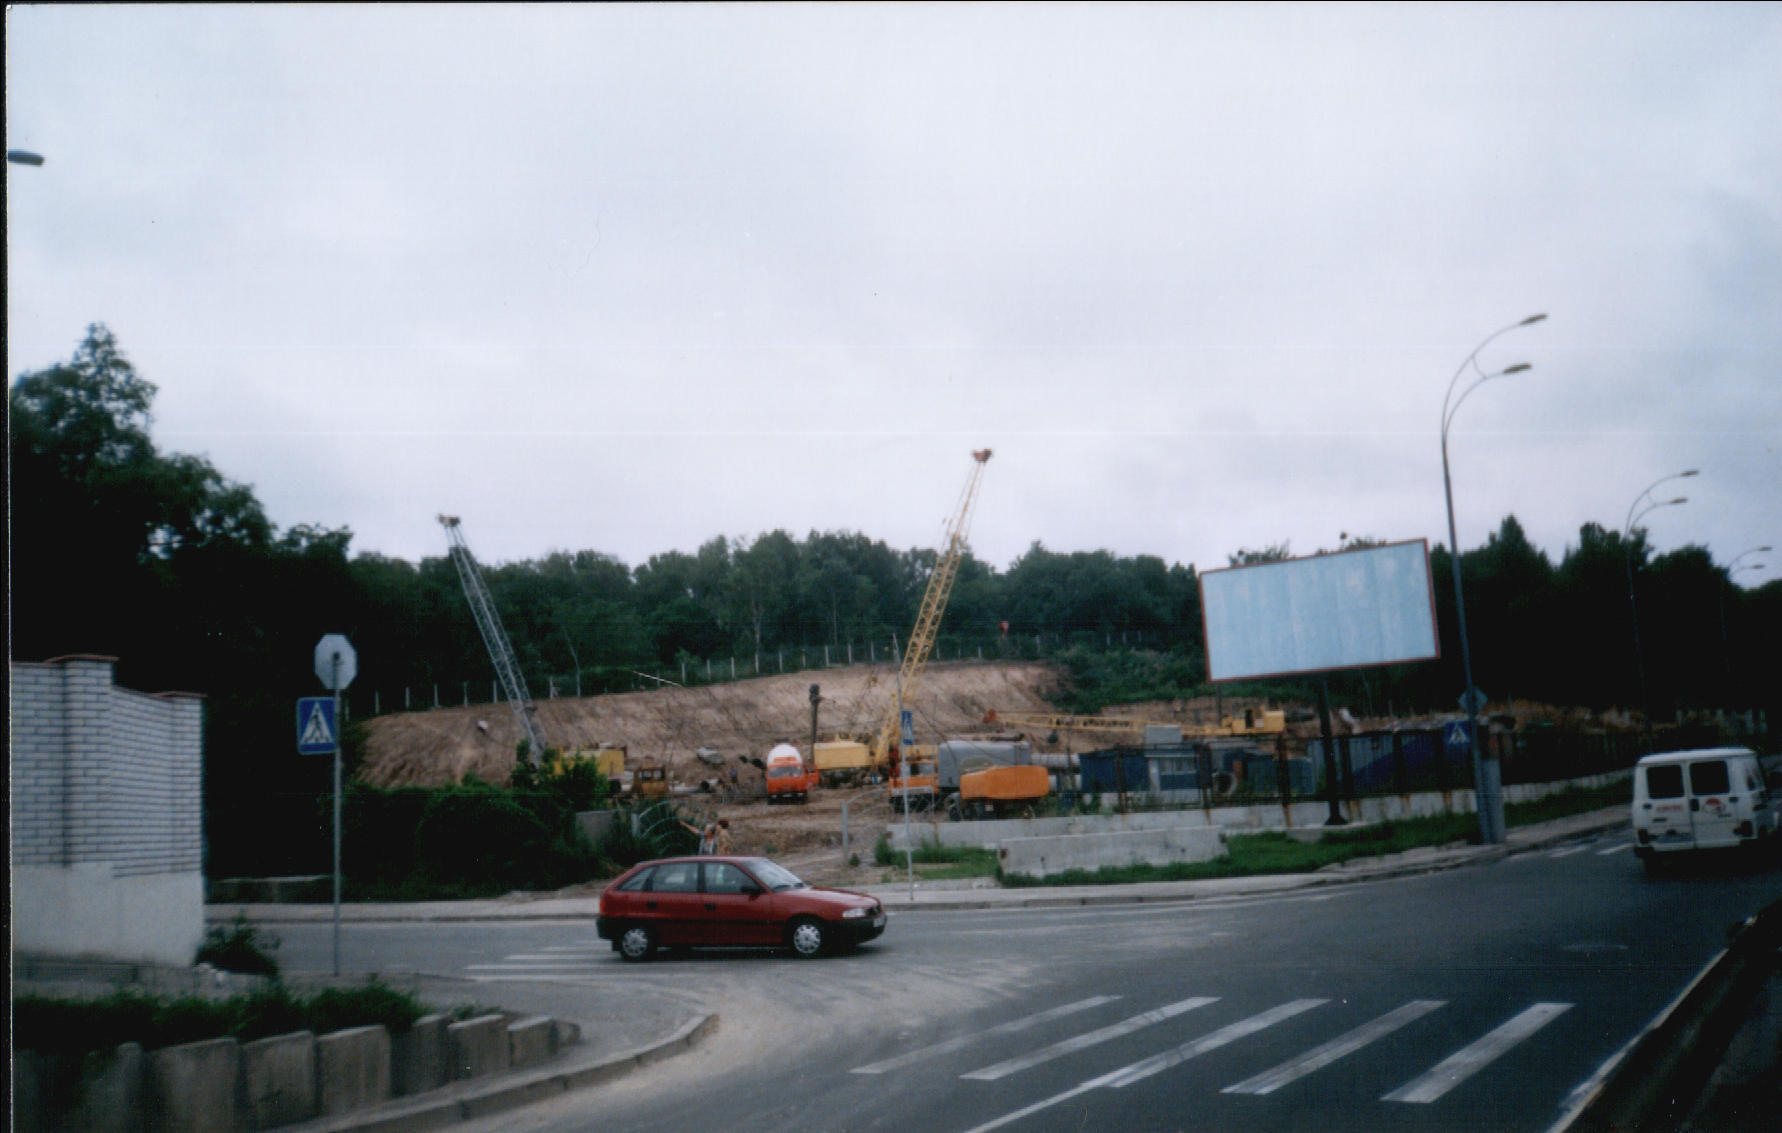
\includegraphics[width=\linewidth]{chast-colebanie-osnov/nachalo/zverinec-niz.jpg}
\end{center}

\vspace*{\fill}

\newpage

Лишь в 2016 году я, занявшись историей киевских кирпичей, узнал, что в конце 18, начале 19 веков там был карьер, где добывалась глина для кирпичного завода. При подобных обстоятельствах, когда в земле обнажаются древнейшие слои, археолог Викентий Хвойка нашел в глинище кирпичного завода Ионы Зайцева ставшую знаменитой Кирилловскую стоянку – в холме, как в слоеном пироге, один на другом покоились слои разных времен. Кости десятков мамонтов, первобытные каменные орудия.
 
А ведь если бы археологи спросили нас с мамой, где мы нашли «штуковину», коли знали б они историю местности – про завод кирпичный – сколько бы еще древностей удалось там найти? Может, «штуковина» была только ключиком к находке, сопоставимой с Кирилловской стоянкой! 

Наука безразличием похоронила открытие. Ученые сидели от него всего в полутора километрах, за толстыми монастырскими стенами. Пешком каждый день можно было ходить изучать. Но предпочитали ездить в Крым, за амфорами.

Киеву же примерно тогда же, в 1982-м, положили 1500 лет от роду, истолковав устроение Кием, братьями его да сестрой общей крепости – «града» по месту своего жительства – как основание с нуля большого поселения.

Празднование этого юбилея города я помню хуже, чем Олимпиаду 1980 года, хотя в первом случае мне было пять лет, а в последнем три. 

Про Олимпиаду встает перед глазами не её символ – олимпийский мишка, но другое. Как по той же улице Тимирязевской бегут ручьи, весной снег таять начал. А к Олимпиаде в Союзе выпустили небывалые фруктовые джемы. В маленьких квадратных коробочках. Из них получались замечательные кораблики. Я ставил в ручеек коробочку и шел рядом, наблюдая, как ее несет чуть ли не до самого хоздвора! Хоздвор знаменит. Там сеялки, веялки, теплицы и старые, выгоревшие от солнца здания сталинских времен. А по пути к нему еще магазинчик от ботсада. Продавались растения – комнатные, огородные и саженцы деревьев. Пахло цветами и черноземом.

Я не знал тогда, что чуть выше по склону, там где участок вьющихся растений, прежде было большое еврейское кладбище. Его снесли, а на месте разбили обсаженные гортензией и клематисом дорожки из бетонных плит. Среди них кое-где попадаются иудейские надгробия, по ним шагают, не замечая.

Можно пройти в самую даль участка и отведать дальневосточного крыжовника – актинидию, крупную и сладкую. Эта лиана цепляется за особую металлическую клеть-опору. Она ржавая, и столбы у навеса над скамейками тоже ржавые. Когда я лазал по ним вверх, а потом спускался, то ладони становились бурыми.

Аллеи, проходящие по бывшим улицам, скрыли прошлое. 

Напротив входа в ботсад стоит Институт проблем прочности. Раньше он раз в неделю завывал на всю округу некой опытной установкой. Местные жители и не догадываются, что всё это было огромным Братским кладбищем, где хоронили погибших в Первую мировую. И в нижней его террасе вырыты погреба хрущовок на улице Подвысоцкого. 

Нынче у меня выработалось как бы историческое зрение. Попав на местность и зная её былое, я чувствую окружающее в настоящем и смутно – в прошедшем времени. А раньше иначе. Было только настоящее и набор привычных, известных каждому, представлений. Братья Кий, Хорив и Щек, да сестра их Лыбедь. Каким-то образом, в седую старину, основали Киев...

Лет в восемнадцать я вычитал где-то цитату из «Повести временных лет» с другим вариантом основания Киева – мол, жил такой перевозчик Кий, переправлял через Днепр, и говорили – «на перевоз на Киев». Однако летописец Нестор сам же эту гипотезу опровергал.

На улице Бастионной 8/2, за углом почты, был мой любимый книжный магазин. Родной. Его после развала Советского Союза переоборудовали в стрип-клуб. В бытность книжного, одним из запомнившихся там моих приобретений начала девяностых стал репринтный томик в мягкой обложке, первого краеведа киевского, Максима Берлинского – «Краткое описание Киева».

Непривычно было «дореформенное» правописание, кажущиеся мне нескладными слова вроде «страховитый», но я прочёл книгу на одном дыхании. К сожалению, перепечатанная в ней карта Киева была махонькой и потому малополезной даже при рассмотрении через увеличительное стекло.

В «Описании» говорилось, со ссылкой на неведомого мне тогда Татищева, что сарматское слово «кивы» означает «горы». И что у впадения Десны в Днепр был город Азагориум, Загорье. Возникло противоречие – так Киев назван по имени князя Кия или от сарматского слова? И если Азагориум, при чем тут «кивы»? Я не стал решать этот вопрос. Принял к сведению, и ладно.

В конце девяностых в Киеве, близ станции метро Петровка, появился одноименный книжный рынок. Туда поначалу переселились торговцы с прежнего, еще «перестроечного», рожденного в 1989 году книжного базара на Куренёвском, или Птичьем рынке. Впрочем, на Птичке по нулевые, не знаю как сейчас (давно не был), существовала небольшая букинистическая толкучка. Со временем на Петровке стали продавать диски с музыкой, программами, фильмами, а затем там образовалась и барахолка как на Куренёвке – да кстати Петровка не так уж далека от нее.

Раньше я часто посещал Петровку, а нынче езжу редко. Покупаю там на букинистических раскладках, в основном где старые книги разложены прямо на асфальте или как щенки-дворняжки выглядывают из коробки. Бывало, возвращался домой с полным рюкзаком, набитым дешевыми и ценными для меня изданиями.

Но миновали светлые времена. Чудесные россыпи хороших подержанных книг по копеечной цене превратились, большей частью, в скопления быстро пожелтевшей перестроечной кооперативной и современной макулатуры.

И вот однажды, когда мой интерес к киевоведению только просыпался, я взял на Петровке книжку в мягкой серой обложке, «Древняя Русь и Киев в летописных преданиях и легендах», Николая Федоровича Котляра. Киев, Наукова думка, 1986 год, цена 30 копеек, 160 страниц, тираж 70000. Современные писатели, завидуйте размаху советской книгопечати.

В работе Котляра я наткнулся на любопытную выдержку, впрочем прерываемую сочинителем и предваренную его оценкой – «встречаем забавную историю, выдуманную, скорее всего, в Новгороде».

А речь шла о том, что Кий, Хорив, Щек и сестра их Лыбедь были разбойниками из Новгорода.
